% \iffalse meta-comment
%
% Copyright (C) \the\year by Liu Benyuan <liubenyuan@gmail.com>
% This file may be distributed and/or modified under the
% conditions of the LaTeX Project Public License, either
% version 1.2 of this license or (at your option) any later
% version. The latest version of this license is in:
%
% http://www.latex-project.org/lppl.txt
%
% and version 1.2 or later is part of all distributions of
% LaTeX version 1999/12/01 or later.
%
% \fi
% 
% \iffalse
% <package>\NeedsTeXFormat{LaTeX2e}[1999/12/01]
% <package>\ProvidesPackage{nudtpaper}
% <package>		[2009/08/12 v1.0 By Liu Benyuan <liubenyuan@gmail.com>]
%<*driver>
\ProvidesFile{nudtpaper.dtx}[2009/08/12 v1.0 NUDT]
\documentclass[11pt]{ltxdoc}
\usepackage{nudtx}
\EnableCrossrefs
\CodelineIndex
\RecordChanges
\begin{document}
  \DocInput{\jobname.dtx}
\end{document}
%</driver>
% \fi
% 
% \def\thuthesis{\textsc{Thu}\-\textsc{Thesis}}
% \def\nudtpaper{\textsc{Nudt}\-\textsc{Paper}}
% 
% \CheckSum{1204}
% \CharacterTable
%  {Upper-case    \A\B\C\D\E\F\G\H\I\J\K\L\M\N\O\P\Q\R\S\T\U\V\W\X\Y\Z
%   Lower-case    \a\b\c\d\e\f\g\h\i\j\k\l\m\n\o\p\q\r\s\t\u\v\w\x\y\z
%   Digits        \0\1\2\3\4\5\6\7\8\9
%   Exclamation   \!     Double quote  \"     Hash (number) \#
%   Dollar        \$     Percent       \%     Ampersand     \&
%   Acute accent  \'     Left paren    \(     Right paren   \)
%   Asterisk      \*     Plus          \+     Comma         \,
%   Minus         \-     Point         \.     Solidus       \/
%   Colon         \:     Semicolon     \;     Less than     \<
%   Equals        \=     Greater than  \>     Question mark \?
%   Commercial at \@     Left bracket  \[     Backslash     \\
%   Right bracket \]     Circumflex    \^     Underscore    \_
%   Grave accent  \`     Left brace    \{     Vertical bar  \|
%   Right brace   \}     Tilde         \~}
%
% \changes{v0.99}{2009/08/12}{Initial Release}
%
% \GetFileInfo{\jobname.dtx}
% 
% \DoNotIndex{\begin,\end,\begingroup,\endgroup}
% \DoNotIndex{\ifx,\ifdim,\ifnum,\ifcase,\else,\or,\fi}
% \DoNotIndex{\let,\def,\xdef,\newcommand,\renewcommand}
% \DoNotIndex{\expandafter,\csname,\endcsname,\relax,\protect}
% \DoNotIndex{\Huge,\huge,\LARGE,\Large,\large,\normalsize}
% \DoNotIndex{\small,\footnotesize,\scriptsize,\tiny}
% \DoNotIndex{\normalfont,\bfseries,\slshape,\interlinepenalty}
% \DoNotIndex{\hfil,\par,\hskip,\vskip,\vspace,\quad}
% \DoNotIndex{\centering,\raggedright}
% \DoNotIndex{\c@secnumdepth,\@startsection,\@setfontsize}
% \DoNotIndex{\ ,\@plus,\@minus,\p@,\z@,\@m,\@M,\@ne,\m@ne}
% \DoNotIndex{\@@par,\DeclareOperation,\RequirePackage,\LoadClass}
% \DoNotIndex{\AtBeginDocument,\AtEndDocument}
%
% \IndexPrologue{\section*{索引}%
%    \addcontentsline{toc}{section}{索~~~~引}}
% \GlossaryPrologue{\section*{修改记录}%
%    \addcontentsline{toc}{section}{修改记录}}
%
% \renewcommand{\abstractname}{摘~~要}
% \renewcommand{\contentsname}{目~~录}
%
% \title{\textsc{NUDTpaper:}\,\,NUDT研究生学位论文\LaTeX{}模板使用手册\thanks{NUDT \LaTeX{} Thesis Template}}
% \author{刘本源 \\ \texttt{Liubenyuan@gmail.com}}
% \date{\fileversion\ (\filedate)}
%
% \maketitle
% \thispagestyle{empty}
%
% \begin{abstract}
% 本模板旨在提供规范的国防科学技术大学\LaTeX{}写作模板环境,
% 现支持硕士/博士学位论文格式,可以自动生成盲评、制作A3封面。
% \end{abstract}
%
% \vspace{2cm}
% \def\abstractname{免责声明}
% \begin{abstract}\noindent
% \begin{enumerate}
% \item 本模板的发布遵守 \LaTeX{} Project Public License,使用前请认真阅读协议内容
% \item 本模板创立参照官方严格的论文写作手册,并同时参照硕士/博士学位论文\textbf{doc}文档对比修改
% \item 国防科学技术大学对论文写作提供写作指南与官方\textbf{doc}模板,
% 同时提供官方的\LaTeX{}模板,本模板的出发点是方便大家使用专业的高效的论文书写工具,
% 其有点在于注重排版质量、命令规范、使用方便、更新及时,符合论文撰写说明。
% 但任何由于使用本模板而引起的论文格式审查问题均与本模板作者无关。
% \item 任何个人或组织均可以本模板为基础进行修改、扩展,生成新的专用模板,但请严格遵
% 守\LaTeX{} Project Public License 协议
% \item 欢迎提出修改意见
% \end{enumerate}
% \end{abstract}
%
% \clearpage
% \tableofcontents
%
% \clearpage
% \pagenumbering{arabic}
% \pagestyle{mainpage}
%
% \section{快速上手}
% 这部分是专门为那些想快速开始写论文的人准备的。
% \begin{description}
% \item[安装\TeX] 下载最新的\TeX{}live或者C\TeX{}并安装
% \item[字体] 用户需要具备\verb|simsun.ttf|, \verb|simhei.ttf|, \verb|simkai.ttf|,
% \verb|STZHONGS.TTF|, 上述字体都是windows自带的; 除此之外,在网上搜索(或者C\TeX{}
% 论坛)``Adobe Opentype 中文字体'',一搜一大把,确保下载下来Adobe的四款OTF字体:
% 宋,黑,仿宋,楷体。Linux用户可将上述字体复制到\verb|/usr/share/fonts/TTF|下。
% \item[试一试] 解压缩下载的模板,双击makepdf.bat(祈祷一下),如果生成了
% \verb|thesis.pdf|$\rightarrow$
% \item[那么我的那些常用的包都在么?] 你会想我的{\bf Trans}论文可以无缝
% 的复制过来么? 对于这一点,你可以修改\verb|mynudt.sty|来实现。但是{\hei 注意},大部分包
% 都在模板中了,而且{\hei 切记切记},不要擅自改动字体等版面设计,我们继续看$\rightarrow$
% \item[咦,数学公式不是很美观呀] 笔者{\hei 强烈}建议用户使用{\bf mtpro2}宏包的,怎么使用,
% 又有哪些好处,参见bookzh.sty吧!不会错的。好了,我们专注于内容本身吧$\rightarrow$
% \item[开始写了] 所有文件均采用UTF8编码,因此要保证你的\TeX{}编辑器
% (winedt, texworks, texmaker, vim, 记事本($\cdots{}$)等)支持这种编码,
% (经过一番搜索设置后)打开\verb|thesis.tex|,如果看到的是中文$\rightarrow$
% \item[漫长的写作] 手边准备着\LaTeX{}的常用帮助文档(数学,图表,引用等),
% 结合你喜欢的文献管理软件(JabRef等), 漫长的\texttt{编辑,编译,修改,编辑,
% 编译$\cdots$}过程之后,突然有一天发现你写完了$\rightarrow$
% \item[校订] 经过老师师兄师弟师妹齐心协力校正之后,你所做的只是:
% \texttt{生成明评论文,制作明评封面,生成盲评论文,制作盲评封面},
% 装订,上交$\rightarrow$
% \end{description}
% {\color{magenta} Done!}
%
% \section{模板介绍}
%
% \textsc{NUDTpaper} 旨在帮助并且推广\LaTeX{}在国防科技大学论文中的应用,
% 本文将尽可能帮助用户掌握\textsc{NUDTpaper}的安装方法,
% 如果仍旧有不清晰的地方可以参考样例文件或者
% 给作者邮件\footnote{liubenyuan@gmail.com},感兴趣的同学可以帮忙维护模板,
% 这个模板首先符合官方的设计要求,希望同学们在使用后能够提出你们的修改意见。
% 该模板很大程度上参考了6院黄老师sofoot的国防科大博士论文模板,
% 哈工大的\LaTeX{}模板以及清华的Thuthesis
% \footnote{主页:\url{http://thuthesis.sourceforge.net}},
% 有很多使用的帮助、\verb|.cls|中的命令以及版面设置均来自Thuthesis和sofoot的模板,
% 对此的引用表示感谢。
%
% {\color{blue}\fs 模板的作用在于减轻论文写作过程中格式调整的时间,
% 其前提就是遵守模板的用法,不提倡手动更改格式,不建议正文中使用
% 手动调节版面的命令,尤其禁止修改行距和使用\verb|\normalsize|,
% 否则即使使用了\textsc{NUDTpaper}也难以保证输出的论文符合学校规范。}
%
% \section{安装}
% \label{sec:install}
%
% \subsection{下载}
% \textsc{NUDTpaper} 主页:\url{http://nudtpaper.googlecode.com}。
% 模板的更新信息发布在\href{http://bbs.ctex.org}{Ctex论坛}。
% \nudtpaper{}的开发版本同样可以在\textsc{gitorious}上获得。
%
% \subsection{模板的组成部分}
% 下表列出了 \nudtpaper{} 的主要文件及其功能介绍,学习模板的最好办法
% 就是参考thesis.pdf!
% \begin{center}
% \begin{longtable}{l|p{8cm}}
% \toprule
% {\hei 文件(夹)} & {\hei 功能描述}\\\midrule
% \endfirsthead
% \toprule
% {\hei 文件(夹)} & {\hei 功能描述}\\\midrule
% \endhead
% \endfoot
% \endlastfoot
% nudtpaper.ins & 模板驱动文件 \\
% nudtpaper.dtx & 模板文档代码的混合文件\\
% nudtpaper.cls & 模板类文件\\
% nudtpaper.cfg & 模板配置文件\\
% thesis.bib & 参考文献样式文件\\
% \hline
% mynudt.sty & 在这里添加你自己的宏包 \\
% thesis.tex & 示例文档主文件\\
% ref/ & 示例文档参考文献目录\\
% data/ & 示例文档章节具体内容\\
% figures/ & 示例文档图片路径\\
% \textbf{nudtpaper.pdf} & 用户手册(本文档)\\
% \textbf{thesis.pdf} & 示例文档 \\
% \bottomrule
% \end{longtable}
% \end{center}
%
% \subsection{\TeX{}系统的选择}
% 有网络环境的用户推荐安装\href{http://www.tug.org/texlive}{\TeX{}live},
% \href{http://miktex.org}{MiKTeX}或者\href{http://www.ctex.org}{C\TeX},
% 对于无网络环境的,主要是针对教研室用户,推荐{\TeX{}live}或者C\TeX{}完整版,安装
% 过程很简单,一路下一步即可,但是需要\textbf{注意:}
%
% \begin{description}
% \item[字体] TTF选项默认调用Windows系统字体,其中楷体、仿宋需要安装Office;OTF选项需要
% Adobe的商业字体(可以使你的论文更加漂亮!),这些中文字体(宋,黑,仿宋,楷体)可以从
% \href{http://dl.getdropbox.com/u/857066/adobe_chinese_otf.7z}{这里下载},
% 如果上述链接不能使用,请搜索\textsc{Adobe Opentype 中文字体}自行下载。
% 英文字体使用Windows自带。起始更推荐几款Times(Arial)类似的OTF英文字体,可以使用
% 更多排版、段落的字体特性。
% \item[粗宋] 模板中在需要宋体加黑的地方需要使用\textbf{华文中宋}, 即STZHONGS.TTF。
% \item[xeCJK] 无网络环境中,C\TeX{}完整版和\TeX{}live最新版都包括了需要的xeCJK版本。
% \end{description}
%
% \subsection{使用模板}
% \label{sec:install-cls}
% {\hei 注:默认的发行版本已经包含了可以使用的模板环境,
% 包括编译好的cls以及论文样例源文件,
% 想快速上手的话,可以直接参看\verb|thesis.tex|,进行修改。
% 写作的过程就是将你的论文的内容放到\verb|data|文件夹中,
% 图片放到\verb|figures|文件夹中,用\textsc{jabref}修改\verb|thesis.bib|即可。}
%
% 当用户需要编译生成自己的PDF版论文时,需要依次输入:(注意了,如果不是使用nomencl,
% 则无需使用第二个命令)
% \begin{shell}
% $ xelatex thesis
% $ # makeindex -s nomencl.ist -o thesis.nls thesis.nlo
% $ bibtex thesis
% $ bibtex thesis
% $ xelatex thesis
% $ xelatex thesis
% \end{shell}
%
% 而为了简化用户使用,模板中提供了快捷脚本文件:
% \begin{shell}
% # 下面命令可以直接生成thesis.pdf,你可能只需要这步
% C:\> makepdf.bat
% # linux用户可以直接使用makefile
% $ make pdf
% \end{shell}
% 现在,就要进入激动人心的写作过程了。
%
% \section{使用说明}
% \label{sec:how-to-use}
% 首先,一篇论文(电子信息工程专业为例),主要的构成就是
% 封面导言,正文,表格,图片,公式,
% 交叉引用及文献索引这五部分,下面将分别详细讲解。
%
% \label{sec:howtoask}
% 在开始之前,先问自己几个问题:
% \begin{compactenum}
% \item 我是不是已经掌握了 \LaTeX{} 基础知识?
% \item 我是不是认真地阅读了模板文档?
% \item 周围有没有同学可以帮我?
% \end{compactenum}
% 更推荐用户去阅读示例文档的源代码,改写会给你一个快速的开始。
%
% \subsection{示例文件}
% \label{sec:example}
% 该示例文件是顶层的文件,包括论文属性设置、章节的安排、参考文献附录等。
% 细节用户可以参考\verb|thesis.tex|和\verb|data/|文件夹。
%
% \subsubsection{模板选项}
%
% 论文的第一句话是调用模板:
% \changes{v2.0}{2010/11/10}{增加盲评的说明}
%
%    \begin{macrocode}
%<thesis>%1. 规范硕士导言
%<thesis>% \documentclass[master,ttf]{nudtpaper}
%<thesis>%2. 规范博士导言
%<thesis>% \documentclass[doctor,twoside,ttf]{nudtpaper}
%<thesis>%3. 如果使用是Vista
%<thesis>% \documentclass[master,ttf,vista]{nudtpaper}
%<thesis>%4. 建议使用OTF字体获得较好的页面显示效果
%<thesis>%   OTF字体从网上获得,各个系统名称统一,不用加vista选项
%<thesis>%   如果你下载的是最新的(1201)OTF英文字体,建议修改nudtpaper.cls,使用
%<thesis>%   Times New Roman PS Std
%<thesis>% \documentclass[doctor,twoside,otf]{nudtpaper}
%<thesis>%5. 如果想生成盲评,传递anon即可,仍需修改个人成果部分
%<thesis>% \documentclass[master,otf,anon]{nudtpaper}
%<thesis>%
%    \end{macrocode}
%    \begin{macrocode}
%<*thesis>
\documentclass[master,otf]{nudtpaper}
\usepackage{mynudt}

%</thesis>
%    \end{macrocode}
%
% 模板的参数设置(开关)描述见:
%
%\begin{description}
%\item[master,doctor]
% 硕士论文用master,博士论文就用doctor
%\item[twoside]
% 指定论文为单面打印还是双面打印,当使用\verb|twoside|选项之后,
% 论文会将章节开在奇数页右手边,默认为\verb|openany|单面打印。
%\item[ttf,otf]
% 决定使用何种字体,TTF默认使用Windows自带的字体,而OTF则使用Adobe的字体(需要下载),
% TTF字体的优势是满足学校论文对于字体的要求,缺点是制作出来的PDF文件在浏览时可能发虚,
% 而OTF字体屏幕显示饱满,而且字体有很多选项可以方便\XeTeX{}排版。推荐使用\textbf{otf}
% 选项。不论何种选项,都需要安装宋体中宋(STZHONGSONG)字体(Windows自带)。
%\item[vista]
% 使用\textsc{vista}的用户当调用模板的TTF字体时,系统默认的楷体、仿宋名称是KaiTi和FangSong,
% 而不是KaiTi\_GB2312,这里加入开关进行切换。
%\item[anon]
% 是否为盲评版本,如需盲评,请加上anon。
%\end{description}
%
% 如果需要使用自己定义的命令、宏包,请放于\verb|mynudt.sty|中。
% 事实上,该文件中已经添加了很多有用的宏包和命令,你可以参照修改。
% 这些之所以没有放到模板中,一则为了简洁,二则赋予用户在格式之外更多的自由。
% 里面的宏包有:代码高亮、算法环境、向量命令等,请仔细查看。
%
% 样例文件默认的是硕士论文(master),OTF字体(otf)。
%
% \subsubsection{封面导言}
% 官方模板中设计论文题目、作者等信息可以跟填空一样完成:
%
% \begin{description}
% \item[论文封头]
% 主要有四部分内容,中图分类号,学号,论文密级和UDC。
% 密级分为:\textbf{秘密} 或者 \textbf{公开}。
%    \begin{macrocode}
%<*thesis>
\classification{TP957}
\serialno{0123456}
\confidentiality{公开}
\UDC{}
%</thesis>
%    \end{macrocode}
%
% \item[论文题目,作者,日期]
% 分别包括中文和英文两部分,由于论文题目可能超过1行,
% 我们提供额外的一个命令\verb|\displaytitle|用来在
% 授权书中填入(限定为)单行的题目; 中文日期需要中文输入大写,英文日期为月年,
% 在论文最终完成后,请\textbf{手动}设定日期。
%
%    \begin{macrocode}
%<*thesis>
\title{国防科大学位论文\LaTeX{}模板\\
使用手册}
\displaytitle{国防科学技术大学学位论文\LaTeX{}模板}
\author{张三}
\zhdate{\zhtoday}
\entitle{How to Use the \LaTeX{} Document Class for NUDT Dissertations}
\enauthor{Zhang San}
\endate{\entoday}
%</thesis>
%    \end{macrocode}
%
% \item[论文分类及其他]
% 主要是作者的学科类别,研究方向,导师信息等。
% 每一项都包括中英文信息:
%
%    \begin{macrocode}
%<*thesis>
\subject{通信与信息工程}
\ensubject{Information and Communication Engineering}
\researchfield{自动目标识别与模糊工程}
\supervisor{李四\quad{}教授}
\cosupervisor{王五\quad{}副教授} % 没有就空着
\ensupervisor{Professor Li Si}
\encosupervisor{}
\papertype{工学}
\enpapertype{Engineering}
%</thesis>
%    \end{macrocode}
%
% \item[中英文摘要]
% 论文中需要写中文以及英文摘要,页码为小写罗马字母,关键字为黑体,
% 英文关键字为\verb|Arial|,
% 模板中定义了相关环境\verb|\cabstract|以及\verb|\eabstract|来书写摘要,
% 以及\verb|\ckeywords|以及\verb|\ekeywords|来写关键字。
% 建议用户将摘要单独放在在\verb|abstract.tex|文件中,
% 在正文中\verb|\begin{cabstract}
现在的互联网上社交媒体随处可见,这给信息检索和传播分析工作带来了机遇与挑战。本文主要围绕在社交媒体中如何找到重要的信息以及信息是如何传播的展开。我们将Twitter作为研究对象,因为它是目前最著名的社交媒体之一,并且数据是公开的。这样从隐私的角度考虑,获取研究数据变得容易且能很好的为研究任务(如信息检索)服务。

信息检索的主要任务是在文档集合中,找到与给定话题相关的客观文本或主观文本。Twitter是一个丰富的包含各种话题及其评论信息的资源库,本文将探讨如何在Twitter中找到相关的信息。但是tweet的短小化和非正式的文本特点,使得Twitter中的检索不同于以往的检索任务(如,网页检索)。本文将通过研究tweet文本特点和特有的Twitter社交媒体属性帮助Twitter检索。另外,Twitter中信息的传播是一种普遍现象且与消息的质量相关(帮助Twitter中检索高质量的信息)。因此,我们从tweet本身和用户的角度,研究哪些因素影响了tweet的转发和人的转发行为。

我们的工作主要有四个部分:(1)利用结构化信息的Twitter检索;(2)Twitter观点检索; (3)Twitter中传播观点的发现;(4)Twitter中信息传播者的发现。四个工作具体如下:

\textbf{利用结构化信息的Twitter检索:} \emph{Twitter检索是在Twitter中找到与给定话题相关的tweet的任务}。绝大部分的Twitter检索系统在构造检索模型时一般都认为tweet是一个平面文本,但用户在编辑tweet时的一些习惯使得tweet文本呈现结构化的特点。这种结构化是通过一些不同的文本积木块组合而成,积木类型具体包括平面文本、主题词、链接、提及等。每一种积木都有自己独特的本质,一系列积木的排序组合又反映了一定的话语转换。以往的研究发现,通过开发文本的结构信息能够帮助结构化文本的检索(例如,网页检索)。本工作通过积木结构开发tweet的结构化信息,以此帮助Twitter检索。我们利用积木及其排列组合开发了一系列特征,并将其应用到排序学习的框架中。我们发现利用结构化tweet的方法进行检索能够达到目前最好的Twitter检索方法效果,将结构化tweet的方法和其他社交媒体特征一起使用能够进一步提高Twitter的检索效果。

\textbf{Twitter观点检索:} \emph{观点检索是在数据中找到对指定话题表达正面或反面观点的tweet的任务}。人们几乎在Twitter中表达了任何话题的观点,使其成为一个丰富的观点资源库。但是Twitter中也存在大量的垃圾信息和各种不同类型的文本,使得Twitter中的观点检索充满挑战。我们提出了如何利用tweet的社交媒体信息和文本结构化信息的方法帮助Twitter的观点检索。特别的,基于排序学习,我们发现tweet的用户信息(如用户包含朋友的数目)、tweet文本本身的结构信息和观点化程度影响着tweet的排序结果。实验结果表明社交媒体信息能够帮助Twitter的观点检索。基于无监督学习评价tweet观点化程度,并以此开发特征形成的检索方法能够到达手工标注tweet的有监督方法的检索效果,且这种方法能够帮助观点检索中话题依赖问题的解决。最后,我们在重新标注的TREC Tweets2011数据集上进一步验证了我们Twitter观点检索方法的有效性。

\textbf{Twitter中传播观点的发现:} Twitter已经变成人们收集观点做出决策的重要资源,但是数量众多且差异巨大的观点严重影响了人们使用这些资源的效果。本文我们考虑了\emph{如何在Twitter中找到传播观点的任务---tweet不仅表达了对某些话题的观点,且这个tweet在未来会被转发}。利用排序学习模型,我们开发了一系列特征,具体包括tweet的传播度特征、观点化特征和文本质量特征。实验结果证明了我们开发的特征对于Twitter中传播观点的发现是有效的,并且将所有特征整合的方法在发现效果上能够显著优于BM25方法和Twitter观点检索方法。最后,我们发现我们的方法在预测观点传播上可以达到人预测的水平。

\textbf{Twitter中信息传播者的发现:} Twitter和其它社交网络中一个重要的交流机制就是消息传播---人们分享其他人创建的消息。虽然目前有许多工作研究了Twitter中的tweet是如何传播的(转发),但是一个未解决的问题是到底\textbf{谁}会转发给定的tweet。这里我们考虑了\emph{在Twitter中给定一条tweet,发现作者的粉丝中谁会转发}。利用排序学习模型的框架,我们设计了一些特征,包括用户历史的转发信息,用户自身的社交媒体特征,用户使用 Twitter的活跃时间,以及用户的个人兴趣 。我们发现经常转发和提及作者的粉丝和与作者有相同兴趣爱好的人最有可能成为信息传播者。

通过以上四个问题的研究,我们发现tweet的文本信息和Twitter的社交媒体特征能够帮助Twitter信息检索和传播分析。

\end{cabstract}
\ckeywords{Twitter; 信息检索; 观点检索; 传播观点; 信息传播者}

\begin{eabstract}


Social Media is now ubiquitous on the internet, generating both new possibilities and new challenges in information retrieval and propagation analysis. This thesis focus on finding important information and propagated information analysis in Social Media. We take Twitter as our research subject, since it is one of the most Social Media and  public by default, which makes the data less problematic from a privacy standpoint, far easier to obtain
and more amenable to target applications (such as information retrieval). 

The main tasks in information retrieval are finding related objective or subjective documents about some topics in collection. Twitter is rich resource which contains information about various topics and opinions. Here we investigate how to find these information in Twitter. However, Twitter retrieval is different from traditional retrieval tasks (e.g, web search), since the text of tweet is short and informal. In this study we exploit textual features of tweet and the social media features to improve Twitter retrieval. Additionally, information dissemination is a prevalent phenomenon in Twitter and is related to the quality of message (which can help finding high quality information in Twitter). Therefore, from the point of view of tweets and users, we study the factors which affect tweet retweeting and users' retweeting behavior.
 
Our work can be divided into four parts: (1) improving Twitter retrieval by exploiting structural information, (2) opinion retrieval in Twitter, (3) finding propagated opinion in Twitter, (4) finding retweeters in Twitter. We introduce the four work in detail as follows:

\textbf{Improving Twitter retrieval by Exploiting structural information}. \emph{Twitter retrieval deals with finding related tweets about some topics in Twitter.} Most Twitter search systems generally treat a tweet as a plain text when modeling relevance. However, a series of conventions allows users to tweet in structural ways using combination of different blocks of texts. These blocks include plain texts, hashtags, links, mentions, etc. Each block encodes a variety of communicative intent and sequence of these blocks captures changing discourse. Previous work shows that exploiting the structural information can improve the structured document (e.g., web pages) retrieval. In this study we utilize the structure of tweets, induced by these blocks, for Twitter retrieval. A set of features, derived from the blocks of text and their combinations, is used into a learning-to-rank scenario. We show that structuring tweets can achieve state-of-the-art performance. Our approach does not rely upon social media features, but when we do add this additional information, performance improves significantly. 

\textbf{Opinion retrieval in Twitter}. \emph{Opinion retrieval deals with finding relevant documents that
express either a negative or positive opinion about some topics}.  
Social Networks such as Twitter, where people routinely post
opinions about almost any topic, are rich environments for opinions. 
However, spam and wildly varying documents makes opinion retrieval
within Twitter challenging. Here we demonstrate how we can exploit 
social  and structural textual information of tweets and 
improve Twitter-based opinion retrieval.  In particular, within 
 a learning-to-rank
technique, we explore the question of whether aspects of an author
(such as the number of friends they have), information derived from
the body of tweets and opinionatedness ratings of tweets can improve performance.
 Experimental results show that social features can improve retrieval
 performance.  Retrieval using a novel unsupervised opinionatedness
feature achieves comparable
performance with a supervised method using manually tagged
Tweets. Topic-related specific structured Tweet
sets are shown to help with query-dependent opinion retrieval. Finally, we
further verify the  effectiveness of our approach for opinion retrieval in re-tagged TREC Tweets2011 corpus.

\textbf{Finding Propagated opinions in Twitter}. Twitter has become an important source for people to collect opinions to make decisions. However the amount and the variety of opinions constitute the major challenge to using them effectively. Here we consider the problem of \emph{finding propagated opinions -- tweets that express an opinion about some topics, but will be retweeted}. Within a learning-to-rank framework, we explore a wide spectrum of features, such as retweetability, opinionatedness and textual quality of a tweet. The experimental results show the effectiveness of our features for this task. Moreover the best ranking model with all features can outperform a BM25 baseline and state-of-the-art for Twitter opinion retrieval approach. Finally, we show that our approach equals human performance on this task.

\textbf{Finding retweeters in Twitter}. An important aspect of communication in Twitter (and other Social Networks) is
message propagation -- people creating posts for others to share.
Although there has been work on modelling how tweets
in Twitter are propagated (retweeted), an
untackled problem has been \textbf{who} will retweet a message. Here 
we consider the task of \emph{finding who will retweet a message posted on Twitter}. Within a learning-to-rank framework, we explore 
a wide range of features, such as retweet history, followers status, followers active time and followers interests. We find that 
followers who retweeted or mentioned the author's tweets frequently before and have common interests are more likely to be 
retweeters.

Based on the study of four work above, we find the textual information of tweet and social media features in Twitter can help Twitter retrieval and propagation analysis.
\end{eabstract}
\ekeywords{Twitter; Information Retrieval; Opinion Retrieval; Propagated Opinion; Retweeter}

|即可。其格式为:
%
% \begin{example}
% \begin{cabstract}
% 中文摘要
% \end{cabstract}
% \ckeywords{关键字}
%
% \begin{eabstract}
% Abstract
% \end{eabstract}
% \ekeywords{Key}
% \end{example}
% \end{description}
%
% \subsubsection{框架构成}
%
% 在定义完论文元素之后,就可以开始写论文正文了。用\LaTeX{}写论文的文件目录构成
% 可以很随意,模板中将图形文件单独放到一个目录中\verb|figure|中,论文正文各个
% 章节置于\verb|data|中;当然也以以\verb|chapter|为目录。
%\changes{v2.2}{2011/05/27}{使用nomencl包管理符号列表}
%\changes{v2.2}{2011/07/08}{默认使用nomencl管理参考文献}
%\changes{v2.2}{2011/09/10}{回复原先使用的denotation方式添加符号列表}
% 
% 如果使用nomencl制作符号列表,在文档开始前要加入\verb|\makenomenclature|命令
% 默认还是使用denotation的方式。nomencl可以参考第二章相关章节,而denote方式
% 请参考\verb|data/denotation.tex|文件(简单的列表环境)。
% 
%<thesis>% 加入makenomenclature命令可用nomencl制作符号列表。
%
%    \begin{macrocode}
%<*thesis> 

\begin{document}
\graphicspath{{figures/}}
%</thesis>
%    \end{macrocode}
% 制作完封面后就是正文四大部分了,分别为:
%
% \begin{compactenum}
% \item frontmatter: 生成目录,图目录,表目录
% \item midmatter: 摘要,符号列表
% \item mainmatter: 正文,致谢,文献,成果
% \item backmatter: 附录
% \end{compactenum}
%
%<thesis>% 制作封面,生成目录,插入摘要,插入符号列表 \\
%<thesis>% 默认符号列表使用denotation.tex,如果要使用nomencl \\
%<thesis>% 需要注释掉denotation,并取消下面两个命令的注释。 \\
%<thesis>% cleardoublepage% \\
%<thesis>% printnomenclature% \\
%
%    \begin{macrocode}
%<*thesis>
\maketitle
\frontmatter
\tableofcontents
\listoftables
\listoffigures

\midmatter
\begin{cabstract}
现在的互联网上社交媒体随处可见,这给信息检索和传播分析工作带来了机遇与挑战。本文主要围绕在社交媒体中如何找到重要的信息以及信息是如何传播的展开。我们将Twitter作为研究对象,因为它是目前最著名的社交媒体之一,并且数据是公开的。这样从隐私的角度考虑,获取研究数据变得容易且能很好的为研究任务(如信息检索)服务。

信息检索的主要任务是在文档集合中,找到与给定话题相关的客观文本或主观文本。Twitter是一个丰富的包含各种话题及其评论信息的资源库,本文将探讨如何在Twitter中找到相关的信息。但是tweet的短小化和非正式的文本特点,使得Twitter中的检索不同于以往的检索任务(如,网页检索)。本文将通过研究tweet文本特点和特有的Twitter社交媒体属性帮助Twitter检索。另外,Twitter中信息的传播是一种普遍现象且与消息的质量相关(帮助Twitter中检索高质量的信息)。因此,我们从tweet本身和用户的角度,研究哪些因素影响了tweet的转发和人的转发行为。

我们的工作主要有四个部分:(1)利用结构化信息的Twitter检索;(2)Twitter观点检索; (3)Twitter中传播观点的发现;(4)Twitter中信息传播者的发现。四个工作具体如下:

\textbf{利用结构化信息的Twitter检索:} \emph{Twitter检索是在Twitter中找到与给定话题相关的tweet的任务}。绝大部分的Twitter检索系统在构造检索模型时一般都认为tweet是一个平面文本,但用户在编辑tweet时的一些习惯使得tweet文本呈现结构化的特点。这种结构化是通过一些不同的文本积木块组合而成,积木类型具体包括平面文本、主题词、链接、提及等。每一种积木都有自己独特的本质,一系列积木的排序组合又反映了一定的话语转换。以往的研究发现,通过开发文本的结构信息能够帮助结构化文本的检索(例如,网页检索)。本工作通过积木结构开发tweet的结构化信息,以此帮助Twitter检索。我们利用积木及其排列组合开发了一系列特征,并将其应用到排序学习的框架中。我们发现利用结构化tweet的方法进行检索能够达到目前最好的Twitter检索方法效果,将结构化tweet的方法和其他社交媒体特征一起使用能够进一步提高Twitter的检索效果。

\textbf{Twitter观点检索:} \emph{观点检索是在数据中找到对指定话题表达正面或反面观点的tweet的任务}。人们几乎在Twitter中表达了任何话题的观点,使其成为一个丰富的观点资源库。但是Twitter中也存在大量的垃圾信息和各种不同类型的文本,使得Twitter中的观点检索充满挑战。我们提出了如何利用tweet的社交媒体信息和文本结构化信息的方法帮助Twitter的观点检索。特别的,基于排序学习,我们发现tweet的用户信息(如用户包含朋友的数目)、tweet文本本身的结构信息和观点化程度影响着tweet的排序结果。实验结果表明社交媒体信息能够帮助Twitter的观点检索。基于无监督学习评价tweet观点化程度,并以此开发特征形成的检索方法能够到达手工标注tweet的有监督方法的检索效果,且这种方法能够帮助观点检索中话题依赖问题的解决。最后,我们在重新标注的TREC Tweets2011数据集上进一步验证了我们Twitter观点检索方法的有效性。

\textbf{Twitter中传播观点的发现:} Twitter已经变成人们收集观点做出决策的重要资源,但是数量众多且差异巨大的观点严重影响了人们使用这些资源的效果。本文我们考虑了\emph{如何在Twitter中找到传播观点的任务---tweet不仅表达了对某些话题的观点,且这个tweet在未来会被转发}。利用排序学习模型,我们开发了一系列特征,具体包括tweet的传播度特征、观点化特征和文本质量特征。实验结果证明了我们开发的特征对于Twitter中传播观点的发现是有效的,并且将所有特征整合的方法在发现效果上能够显著优于BM25方法和Twitter观点检索方法。最后,我们发现我们的方法在预测观点传播上可以达到人预测的水平。

\textbf{Twitter中信息传播者的发现:} Twitter和其它社交网络中一个重要的交流机制就是消息传播---人们分享其他人创建的消息。虽然目前有许多工作研究了Twitter中的tweet是如何传播的(转发),但是一个未解决的问题是到底\textbf{谁}会转发给定的tweet。这里我们考虑了\emph{在Twitter中给定一条tweet,发现作者的粉丝中谁会转发}。利用排序学习模型的框架,我们设计了一些特征,包括用户历史的转发信息,用户自身的社交媒体特征,用户使用 Twitter的活跃时间,以及用户的个人兴趣 。我们发现经常转发和提及作者的粉丝和与作者有相同兴趣爱好的人最有可能成为信息传播者。

通过以上四个问题的研究,我们发现tweet的文本信息和Twitter的社交媒体特征能够帮助Twitter信息检索和传播分析。

\end{cabstract}
\ckeywords{Twitter; 信息检索; 观点检索; 传播观点; 信息传播者}

\begin{eabstract}


Social Media is now ubiquitous on the internet, generating both new possibilities and new challenges in information retrieval and propagation analysis. This thesis focus on finding important information and propagated information analysis in Social Media. We take Twitter as our research subject, since it is one of the most Social Media and  public by default, which makes the data less problematic from a privacy standpoint, far easier to obtain
and more amenable to target applications (such as information retrieval). 

The main tasks in information retrieval are finding related objective or subjective documents about some topics in collection. Twitter is rich resource which contains information about various topics and opinions. Here we investigate how to find these information in Twitter. However, Twitter retrieval is different from traditional retrieval tasks (e.g, web search), since the text of tweet is short and informal. In this study we exploit textual features of tweet and the social media features to improve Twitter retrieval. Additionally, information dissemination is a prevalent phenomenon in Twitter and is related to the quality of message (which can help finding high quality information in Twitter). Therefore, from the point of view of tweets and users, we study the factors which affect tweet retweeting and users' retweeting behavior.
 
Our work can be divided into four parts: (1) improving Twitter retrieval by exploiting structural information, (2) opinion retrieval in Twitter, (3) finding propagated opinion in Twitter, (4) finding retweeters in Twitter. We introduce the four work in detail as follows:

\textbf{Improving Twitter retrieval by Exploiting structural information}. \emph{Twitter retrieval deals with finding related tweets about some topics in Twitter.} Most Twitter search systems generally treat a tweet as a plain text when modeling relevance. However, a series of conventions allows users to tweet in structural ways using combination of different blocks of texts. These blocks include plain texts, hashtags, links, mentions, etc. Each block encodes a variety of communicative intent and sequence of these blocks captures changing discourse. Previous work shows that exploiting the structural information can improve the structured document (e.g., web pages) retrieval. In this study we utilize the structure of tweets, induced by these blocks, for Twitter retrieval. A set of features, derived from the blocks of text and their combinations, is used into a learning-to-rank scenario. We show that structuring tweets can achieve state-of-the-art performance. Our approach does not rely upon social media features, but when we do add this additional information, performance improves significantly. 

\textbf{Opinion retrieval in Twitter}. \emph{Opinion retrieval deals with finding relevant documents that
express either a negative or positive opinion about some topics}.  
Social Networks such as Twitter, where people routinely post
opinions about almost any topic, are rich environments for opinions. 
However, spam and wildly varying documents makes opinion retrieval
within Twitter challenging. Here we demonstrate how we can exploit 
social  and structural textual information of tweets and 
improve Twitter-based opinion retrieval.  In particular, within 
 a learning-to-rank
technique, we explore the question of whether aspects of an author
(such as the number of friends they have), information derived from
the body of tweets and opinionatedness ratings of tweets can improve performance.
 Experimental results show that social features can improve retrieval
 performance.  Retrieval using a novel unsupervised opinionatedness
feature achieves comparable
performance with a supervised method using manually tagged
Tweets. Topic-related specific structured Tweet
sets are shown to help with query-dependent opinion retrieval. Finally, we
further verify the  effectiveness of our approach for opinion retrieval in re-tagged TREC Tweets2011 corpus.

\textbf{Finding Propagated opinions in Twitter}. Twitter has become an important source for people to collect opinions to make decisions. However the amount and the variety of opinions constitute the major challenge to using them effectively. Here we consider the problem of \emph{finding propagated opinions -- tweets that express an opinion about some topics, but will be retweeted}. Within a learning-to-rank framework, we explore a wide spectrum of features, such as retweetability, opinionatedness and textual quality of a tweet. The experimental results show the effectiveness of our features for this task. Moreover the best ranking model with all features can outperform a BM25 baseline and state-of-the-art for Twitter opinion retrieval approach. Finally, we show that our approach equals human performance on this task.

\textbf{Finding retweeters in Twitter}. An important aspect of communication in Twitter (and other Social Networks) is
message propagation -- people creating posts for others to share.
Although there has been work on modelling how tweets
in Twitter are propagated (retweeted), an
untackled problem has been \textbf{who} will retweet a message. Here 
we consider the task of \emph{finding who will retweet a message posted on Twitter}. Within a learning-to-rank framework, we explore 
a wide range of features, such as retweet history, followers status, followers active time and followers interests. We find that 
followers who retweeted or mentioned the author's tweets frequently before and have common interests are more likely to be 
retweeters.

Based on the study of four work above, we find the textual information of tweet and social media features in Twitter can help Twitter retrieval and propagation analysis.
\end{eabstract}
\ekeywords{Twitter; Information Retrieval; Opinion Retrieval; Propagated Opinion; Retweeter}


\begin{denotation}

\item[TBB] Twitter积木 (Twitter Building Blocks)
%\item[$\Delta G$]  	活化自由能~(Activation Free Energy)
%\item[$E$] 能量

\end{denotation}


%</thesis>
%    \end{macrocode}
%
%<thesis>%书写正文,可以根据需要增添章节; 正文还包括致谢,参考文献与成果
%\changes{v1.4}{2009/10/31}{将成果移动到参考文献之后}
%
%    \begin{macrocode}
%<*thesis>
\mainmatter
\chapter{绪论}
\label{Intro}

\section{研究背景}

\subsection{社交媒体}
\label{ch1_social}
作为划时代的创新,互联网20年以来已深刻影响和改变着我们的生活,思维和行为方式。尤其现在,我们可以通过手机、各种穿戴式智能设备,随时随地保持与互联网不间断联系。根据中国互联网络信息中心的权威报告,截至2014年7月,我国网民规模达6.41亿,手机网民规模已超过5亿,互联网普及率为47.4\%\footnote{\url{http://www.cnnic.cn/hlwfzyj/hlwfzzx/qwfb/201408/t20140825\_47878.htm}}。
随着互联网技术的迅猛发展,出现了形形色色吸引用户参与的社交媒体(Social Media)平台,并且已经成为人类工作、学习、生活必不可少的重要部分。
%图~\ref{fig1-1}展示了各种国内外的在线社交媒体平台。

%\begin{figure}[htp]
%\centering
%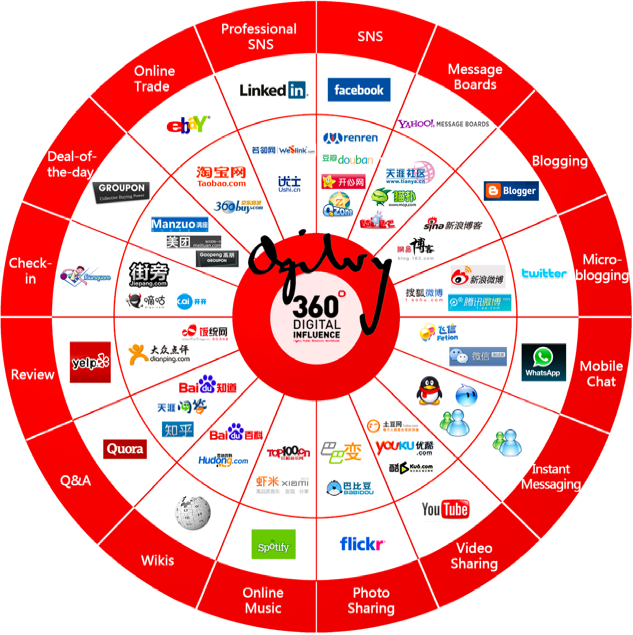
\includegraphics[height=340pt]{1-1.png}
%\caption{国内外社交媒体}
%\label{fig1-1}
%\end{figure}

社交媒体中的互联网用户不再是单纯的信息接收者,同时也是网络内容的产生者,人们通过社交媒体进行交流而获取和产生信息。以中国为例,目前拥有12亿手机用户、5亿微博用户、5亿微信用户,每天信息发送量超过200亿条,交流无处不在,无时不有。表~\ref{tab1-1}是互联网网站信息统计公司Alexa\footnote{网站地址:\url{www.alexa.com},访问时间:2014年9月。}统计的网络访问统计,从表中可以看出,根据统计,流量前十的互联网网站中社交媒体占了绝大部分。

\begin{table}[htp]
\centering
\caption{Alexa统计访问量前十名网站}
\label{tab1-1}
\begin{threeparttable}
 \begin{tabular}{|l|l|l|l|}
 \hline
 排名&网站&排名&网站\\
 \hline
 1& Google.com& 6&\textbf{ Wikipedia.org\tnote{1}}\\
 2& \textbf{Facebook.com}& 7& \textbf{Amazon.com}\\
 3& \textbf{Youtube.com}& 8& \textbf{Twitter.com}\\
 4& Yahoo.com& 9& \textbf{Qq.com}\\
 5& Baidu.com& 10& \textbf{Taobao.com}\\
 \hline
\end{tabular}
\begin{tablenotes}
  \centering
  \footnotesize
\item[1]表中加黑部分为社交媒体
\end{tablenotes}
\end{threeparttable}
\end{table}

那么究竟什么是社交媒体呢?社交媒体的典型代表维基百科是这样定义的\footnote{\url{http://en.wikipedia.org/wiki/Social media/}}:

\begin{definition}[Social Media]
Social media are media for social interaction, using highly accessible and scalable communication techniques. It is the use of web-based and mobile technologies to turn communication into interactive dialogue.
\end{definition}
从定义中我们可以看出,社交媒体是以互联网的思想和技术为基础的一项应用,用户可以借此进行内容创作、情感交流与信息分享。一般来讲,社交媒体可以分为如表~\ref{tab1-2}所示的几种类型。

\begin{table}[htp]
\centering
\caption{社交媒体的类型}
\label{tab1-2}
 \begin{tabular}{|l|l|}
 \hline
 类型& 代表性网站\\
 \hline
 维基(Wiki) & Wikipedia,Scholarpedia,百度百科\\
 \hline
 博客(Blogging) & Blogger,LiveJournal,WordPress,博客\\
 \hline
 新闻(Social News) & Digg, Mixx,Slashdot\\
 \hline
 微博(Micro Blogging) & Twitter,Google Buzz,新浪微博\\
 \hline
 评论(Opinion \& Reviews) & ePinions,Yelp,豆瓣\\
 \hline
 问答(Question Answering) & Yahoo! Answers,百度知道\\
 \hline
 媒体分享(Media Sharing) & Flickr,Youtube,优酷\\
 \hline
 书签(Social Bookmarking) & Delicious,CiteULike\\
 \hline
 社交网络(Social Networking) & Facebook,LinkedIn,MySpace,人人网\\
 \hline
\end{tabular}
\end{table}

从表中可以看出,社交媒体有多中不同类型,因此会产生多种不同形式的信息,包括文本、图像以及视频等。社交媒体上的信息由广大的社交媒体使用者产生,因此称为用户产生内容(User-Generated Content,UGC),这些信息依靠用户之间的关系与交互形成相互关联的庞大数据库。Kaplan和Haenlein\upcite{Kaplan2010}从数据和信息流动角度定义了社交媒体:首先是作为媒体(media),社交媒体中最突出的特点是它区别于电视、广播和报纸等传统媒体(信息的流动是从少数内容生产者到广大的信息消费者),内容产生的权利扩展到了所有的用户,而且信息流动的方式变得不确定,用户可以在内容消费者和生产者之间多次瞬间改变自己的角色;其次,作为社交工具,我们称这种新媒体是社会化的(social)的媒体,社会化意味着信息内容不只是由个体用户产生,更多是与其他用户的协作产生,信息的内容变得更加多样化,因此社交媒体不只是用来产生信息,也成为用户间互相交流通信以及传播信息的便利工具。

虽然社交媒体的出现为我们信息交流提供了便利,但是随着用户数量不断增加,产生的内容达到新的量级,导致我们作为信息消费者遇到了一些新的挑战,使得我们从“信息海洋”中找到有用信息变得更加困难,这通常称为信息超载(information overload)\footnote{信息超载描述了一种状态,就是当一个人在做选择时因为太多的信息而造成决策的困难。}。同时,由于社交媒体发布消息相对廉价和方便,内容产生门槛降低,任何人都能够参与其中,因此社交媒体中的数据出现了不同于传统媒体数据的新特点。
一般来讲,社交媒体中的数据具有以下特点\upcite{eisenstein2013bad}:
\begin{itemize}
\item \textbf{数量巨大(Big):}社交媒体中每个用户产生的数据可能不大,但是因为用户群体数量庞大,整体数据规模不可小觑,比如平均每天有超过300万条的微博(tweets)发布到Twitter\footnote{\url{http://www.twitter.com/}},每分钟有超过3000张照片上传到Flickr\footnote{\url{http://www.flickr.com/}},每年有超过160多万的博客(blogs)发表。
\item \textbf{广泛链接(Linked):}社交媒体的社会化特性使得用户产生的数据天生就是广泛链接的,最直观的就是用户产生内容往往由于用户之间的各种社交关系链接在一起,是一种新形式的大数据。这种链接的数据显然不是独立同分布的(IID,independent and identically distributed),对于想要使用传统的数据挖掘和机器学习方法研究社交媒体的研究人员是一种挑战\upcite{jensen2002linkage,taskar2003label}。
\item \textbf{充满噪声(Noisy):}社交媒体数据产生门槛的降低以及接入手段的增加,使得社交媒体的数据质量参差不齐,充满噪声\upcite{Agichtein2008}。不仅于此,社交媒体中的网络结构也充满噪声,一是网络中存在一些传播虚假和垃圾信息的用户\upcite{stringhini2010detecting},二是用户间建立关系的便捷性使得用户很容易将各种社会关系混杂在一起,无法区分好朋友和陌生人\upcite{xiang2010modeling}。
\item \textbf{非结构化(Unstructured):}社交媒体中用户产生数据,主要是文本数据,是高度非结构化的,尤其是随着移动互联方式的普及,越来越多的用户使用移动设备更新Facebook的状态,发送微博,或者回复别人的帖子,这不但导致了文本内容短小,而且错误拼写频繁出现\upcite{rossion1999spatio},经常还有一些非自然语言的使用,比如表情符(:),:()和缩写(h r u?)等\upcite{speriosu2011twitter}。
\item \textbf{不完整性(Incomplete):}为了保护用户的隐私,社交媒体平台一般允许用户将一些个人数据进行隐藏不被他人看到,这些数据包括个人信息,状态更新,朋友列表,发布的视频和照片以及与他人的信息交流等。比如Facebook仅有很少部分用户(小于1\%)公开了他们的个人数据\upcite{mislove2010you}。因此社交媒体的数据是极度不完整和稀疏的。
\end{itemize}

社交媒体的迅速普及与壮大,使得它在政治、经济、教育、社会等多方面发挥着越来越重要的作用。一些互联网公司开始以社交媒体大数据资源为支撑,以SaaS形式为用户提供服务。典型的如谷歌和Facebook的自助式广告下单服务系统、Twitter基于实时搜索数据的产品满意度分析以及国内百度推出的大数据营销服务 “司南”等。同时,政府也是社交媒体数据的积极使用者,2013年曝光的棱镜门事件显示出美国国家安全部门在使用社交媒体数据应用的强大实力,其应用范围之广、水平之高、规模之大都远远超过人们的想象。白宫2014年5月发布的《大数据:抓住机遇,守护价值》报告中重点提及了社交媒体大数据\footnote{来源:\url{http://www.whitehouse.gov/sites/default/files/docs/big\_data\_privacy\_report\_may\_1\_2014.pdf}}。
社交媒体大行其道的今天,自然也会成为品牌营销的手段之一,比如今年世界杯的主要赞助商之一可口可乐就首次挑选了粉丝在Facebook\footnote{\url{http://www.facebook.com/}}和Twitter上分享的照片,尝试进行iBeacon在社交媒体营销中的运用。
目前常见的社交媒体的大数据应用有:
一是基于用户个人信息、行为、位置、微博等数据而进行的个性化推荐、交叉推荐、品牌监测等营销类大数据应用,被互联网广告、电子商务、微博、视频、相亲等公司普遍采用。
第二,公共服务类大数据应用,即不以盈利为目的、侧重于为社会公众提供服务的大数据应用。典型案例如谷歌开发的流感、登革热等流行病预测应用能够比官方机构提前一周发现疫情爆发状况。国内也有搜索引擎公司提供诸如春运客流分析、失踪儿童搜寻的公益大数据服务。
三是积极借助外部数据,主要是互联网数据,来实现相关应用。例如,金融机构通过收集互联网用户的微博数据、社交数据、历史交易数据来评估用户的信用等级;证券分析机构通过整合新闻、股票论坛、公司公告、行业研究报告、交易数据、行情数据、报单数据等,试图分析和挖掘各种事件和因素对股市和股票价格走向的影响;监管机构将社交数据、网络新闻数据、网页数据等与监管机构的数据库对接,通过比对结果进行风险提示,提醒监管机构及时采取行动;零售企业通过互联网用户数据分析商品销售趋势、用户偏好等等。

随着社交媒体的迅速发展与参与用户的数目不断增多,社交媒体中可使用的信息也越来越丰富,具有广泛的应用前景。但是社交媒体中信息的庞大规模使得手工分析其内容变得十分困难,因此本文从信息自动化处理的角度对社交媒体的信息,主要是文本信息进行挖掘与分析,发现有用的信息,为社交媒体的相关应用提供帮助,本文特别关注社交媒体中的观点信息。
当然社交媒体与传统媒体存在显著的差异,其自身有不同的特点,我们将研究分析其特点为解决观点信息挖掘分析问题找到解决方案。


\subsection{观点分析}
%实际上文本信息有两种:事实信息与观点信息,事实信息是对事物的客观陈述。观点信息通常包含在博客、评论、回复或微博中,一般是由客户、读者或者公众用于表达表达自己的态度(attitudes),评价(appraisals),观点(perspective),情绪(sentiment)和情感(emotions)。用户不仅对产品(product)或服务(service)表达观点,也会对社会生活中各种话题(topic)或议题(issuses)表达自己的观点。
%观点挖掘或情感分析是自然语言处理(natural language processing)、机器学习(machine learning)以及文本挖掘(text mining)跨学科领域的研究,用于分析文本中对于产品、服务、话题或议题发表的观点,也称为情感分析或主观性分析(subjectivity analysis)\upcite{Liu2005}
%观点(opinion)一词起源于”opine“,通常”sentiment, view, feeling, belief, conviction, persuasion, notion, idea, and impression“为其同义词,词典中”opinion“被定义为信念,判断,个人的观点,态度,评价,思想,感觉和情感(belief , judgment , personal view, attitude, appraisal, thought , feeling, and emotion.)。观点的主要特点就是它是私人的感受,不是建立在证据和确定性基础上的。观点最终要有两个部分:目标(target)和情感(sentiment)\upcite{Liu2012}.
%实际生活中,别人的观点在决策过程中有时候是必不可少的信息。比如在商业领域,消费者在选择产品的时候常常需要知道其他人的对这些产品的评价,而商家为了市场营销也需要知道消费者的观点。在政治领域,投票者受到其他人关于候选人看法的影响而决定选择,同时大众的观点也会影响到政策制定者的政策决心。


信息分为两种,即客观信息和主观信息。语言学家Lyons\upcite{Lyons1977}将语言功能分为描述(descriptive), 社交(social)的和表达( expressive)三种功能。其中描述功能主要表达客观事实信息(factual information),而社交和表达功能往往表达的是个人的主观信息(subjective information)。主观信息,在语言中主要表现为观点信息,是人们在语言中表达对于谈论的目标事物的态度、情感或者看法\upcite{Wiebe2004}。观点常常简化为人对目标的同意或不同意(或者认为目标好或者坏,或持积极(positive)态度还是消极(negative)态度)\upcite{Rachels1986}等简单表示形式。总结起来,用户在社交媒体中表达的观点信息有三种类型:在评论、论坛、博客以及微博中针对某主题发表的个人体验(experience)和想法(opinion);关于新闻文章(artitle)、议题(isssues)、话题(topics)发表的评论(comments);在社交网站,比如Facebook上发表的个人状态更新(status)。

以往为了获取用户观点,需要进行问卷调查,而社交媒体的出现,为用户提供了全新的内容共享平台,使大量连接到网络的用户能够在各种社交媒体发表和表达自己观点:比如消费者可以在Amazon\footnote{\url{www.amazon.com}}, Yelp\footnote{\url{www.yelp.com}}, 以及TripAdvisor\footnote{\url{www.tripadvisor.com}}上发表各种商品和服务的评论;用户可以在Twitter\footnote{\url{www.twitter.com}}和Facebook\footnote{\url{www.facebook.com}}上对最新话题表达自己的观点。社交媒体上巨大的用户群以及由他们产生的海量信息成为了分析用户对各种话题所持观点的宝贵资源。
这些观点信息无论是对个人还是机构都起到非常重要作用。比如Horrigan\upcite{Hoffman2008}发现网络中发表的宣传信息对于网络用户在某些话题上观点的形成具有深远影响,用户表达的观点同样也是产品商家\upcite{Horrigan2008}以及政策制定者\upcite{Mullen2006}不得不考虑的重要因素,有证据显示这种观点的相互作用过程具有显著经济效果\upcite{Antweiler2004,Archak2007,Chevalier2006}。此外,大规模的用户看法整合形成的观点可以反映政治倾向\upcite{Tumasjan2010},甚至可以提高股票市场的预测\upcite{bollen2011twitter}。

社交媒体用户产生内容的大容量不可能依靠人工地去发现和总结其中的观点信息,因此需要计算机能够自动对观点信息进行分析和挖掘。观点分析\footnote{本观点分析包括了情感分析(sentiment analysis),观点挖掘(opinion mining)以及主观性分析(subjectivity analysis)等任务,都是对文本中的观点信息进行分析。}(opnion analysis)\upcite{Pang2008OMS}就是对文本中带有情感色彩的主观性信息进行分析、处理、归纳和推理的过程,其目的是自动发现和区分针对目标的情感和观点,目标可以是命名实体、也可以是话题或事件。
尽管语言学和自然语言处理已经有很长的研究历史,但是直到2000年才开始进行观点挖掘和情感分析等观点分析研究,从此观点分析成为了非常活跃的研究领域。特别是由于社交媒体的出现,研究者第一次拥有了大量的具有主观性信息的数据,正是有了这些数据,规模性的观点分析研究成为可能,可以说观点分析与社会媒体是一起起步和成长的,是社交媒体中数据分析的核心研究。观点分析研究不仅对自然语言理解(Natural Language Understanding)有着重要的影响,而且还对管理学,政治学,经济学和社会科学产生深远影响,因为它们都受到人的主观性的影响。

%
%
%观点分析(或观点挖掘)研究逐渐发展成为介于自然语言处理(Natural Language Processing)与自然语言理解(Natural language understanding)之间的一个独立领域,不像其他的自然语言处理任务(文摘或文本分类),观点挖掘主要处理与自然语言概念相关的语义信息和情感信息的推理而不需要对文本进行深度语法分析\upcite{cambria2014jumping}。

%如此巨大的信息量,主要是非结构化的(因为它是专为人类阅读消费产生的),因此不能直接使用机器处理的。文本的自动分析需要由机器对自然语言进行深入理解成,实际上我们距离这个目标还很远\upcite{6710245}。到目前为止,网上信息检索,汇总和处理都依据主要是依靠文本的文字表示方式。这些算法非常擅长于对文本进行检索,将其拆分,检查拼写和计算词语。但是,当涉及到解释的句子,提取有用的信息,他们的能力是非常有限的。这些基于词表示的算法的很大局限就是他们只能处理字面上的信息,而对于人类来讲,我们就不会收到这样的限制,因为我们看到的每一个字激活的语义相关概念,相关的情节和感官体验的级联,所有这些都使得我们可以以快速高效方式完成一些复杂任务(如词义消歧,文字蕴涵和语义角色标注)。计算模型试图通过模仿人类大脑处理自然语言的方式来弥补这样的认知差距,比如利用在未明确表示的文本语义特征。这些计算模型是有用既为科学目的(如探索语言交流的性质),以及用于实际用途(如能够有效地进行人机交流)。计算模型可以提供关于可再由心里语言学家(psycholinguist)进行探索的人类行为非常具体的预测。通过继续在这个过程中,我们可能最终会获得人类怎样进行语言处理深刻的理解。为了实现这样的梦想,需要具有前瞻性的思维心理语言学家,神经科学家,人类学家,哲学家,和计算机科学家的共同努力。
首先针对观点分析研究应该明确以下几个概念:
\begin{definition}[文档(Document)]
文档指的是自然语言中的文本片段,一般文档中至少会讨论一个话题。
\end{definition}
\begin{definition}[话题(Topic)]
本文中的话题可以是命名实体,事件,或者文档中提及的抽象概念(政治、健康、体育等)。
\end{definition}
\begin{definition}[情感(Sentiment)]
情感指的是文档作者针对话题表达的态度(attitude)、观点(opinion)或情绪(emotion)。
\end{definition}
\begin{definition}[情感极性(Polarity)]
情感极性值指的评价观点积极(positive)或消极(negative)程度的度量值,可以是一维的(打分值),二维的(积极值和消极值),也可以是多维的(喜怒哀乐等情感对应值)。
\end{definition}

针对观点有不同的定义方法,Liu\upcite{Liu2012}将观点形式化定义为观点五元组$ (e_i,a_ij,s_ijkl,h_k,t_l)$,
其中,$ e_i $是目标名称,$ a_{ij} $是目标的不同属性(方面,aspect),$ h_k$是持有观点的用户,$ t_l$表示时间,$ s_{jkl}$是观点的情感值。
Kim和Hovy也对观点做了定义\upcite{Kim2004},认为观点由四个元素组成:即主题(Topic)、持有者(Ho1der)、陈述(Claim)、情感(Sentiment)。
他们认为观点分析就是发现和确定各个元素的过程。
总体来看,比较全面的观点分析可以认为是由三个主要步骤组成:
\begin{itemize}
\item \textbf{文本中观点信息确定:}需要确定文档中涉及的话题信息,将不同话题对应的文本片段进行对应联系起来,并且需要对文本片段进行主客观分离找到主观性文本,因为观点一般是从主观性的文本中确定的。将主客观文本分离一般需要一些明显带有情感的词语作为标志,这些词语集合在一起形成了能对情感知识进行表示的情感词典。
\item \textbf{文本情感分类:}从文本中抽取有用的特征将文本分为不同的情感类别,一般是将文本分为积极或消极极性(或者中性,即客观文本),主要使用机器学习的各种方法,或者基于规则的方法。
\item \textbf{观点的集成表示:}经过前面两步,得到了主观文本片段以及文本片段中的具体观点,观点的集成是在更高的层次上的观点分析,是将文本片段中分散的观点整合集成成为一个观点,并根据不同的应用需求以一种合理的方式表示,比如可以见同一作者的所有文本片段中的观点集成起来,称为用户的主观性模型,或者将文本片段按照时间前后串联起来形成观点随时间的演化表示。
\end{itemize}

观点分析有别于传统的话题分析。话题分析关心的是文本所阐述的客观话题,如文档是属于教育类还是娱乐类的,而观点分析主要用来识别文档中表达的观点、喜好、立场和态度等主观信息,需要分析文档的词语语义、词性,甚至句法和篇章结构等信息。在传统的话题分析中,主题词是最重要的特征,而在观点分析中,情感词是最重要的特征。观点分析涉及语言学领域的诸多问题,由于语言的复杂性和多样性,需要面临以下几个问题:

\begin{enumerate}
\item \textbf{领域相关性:}某些情感词在不同的领域中具有不同的情感极性,比如 :``轻薄 '' 在通常意义下具有消极极性,如 ``举止轻薄'',而在电脑领域,``轻薄 ''却表示褒义,具有积极极性。
\item \textbf{语境依赖性:}某些词语具有多个词性,并且不同的词性常常呈现出不同的情感极性。比如``这款空调经济耐用''和 ``经济呈现快速发展'' 在这两句话中,``经济'' 具有不同的词性和情感极性,前者是形容词,具有积极情感极性,后者是名词,具有中性情感极性。
\item \textbf{上下文相关性:}语言中有许多词语本身是不具有情感极性的,但是在特定的上下文环境中,语言描述便具有了情感极性。比如:``小''、``高''、``快'' 等词语,在搭配组合``损失小''、``成绩高''、``进歩快''中,具有积极情感极性,但在搭配组合 ``心眼小''、 ``耗油高''、``耗电快'' 中,则具有消极情感极性。
\end{enumerate}

%情感词典,是人们在表达观点时常用的一些词语,是主观性信息的最明显的证据(比如``好'')。无论对无监督还是监督方法,因此一部好的情感词典是从文本信息中发现主观信息的重要特征。近年来从网络数据中发现主观性信息变得越来越重要,能够获得大家对一些事物、人或事件的主观性态度比仅仅只有百科式描述更重要,比如对产品的问卷调查,政治选举的民调以及商业广告效果分析等。因此很多研究者开始注意到这种信息需求,并试图从网络数据中挖掘并分析主观性信息。然而大多数工作主要关注与于本中情感倾向的总体以及详细的分析,并且仅仅是对某些特定领域的文本数据,比如产品评论或博客,并不适用于其他类型数据。随着社交媒体的普及,用户可以更方便地发表与自己有关的信息,比如自己的生活和对周围食物的观点,这些越来越多的用户产生数据使得主观性信息的挖掘和分析变得更重要。受到这种趋势和研究需求的影响,TREC评测\footnote{\url{http://www.trec.state.tx.us/}}从2006年开始就有关于从网络信息中挖掘观点的评测,并且受到很多自然语言处理研究人员的关注。判断一片文档是否有主观性信息最简单直观的方式就是看看是否含有主观性词语,这种基于词语的判断方式的基本假设就是文档中含有主观性词语通常是表达作者的主观观点,比如在商品评论中出现``喜欢''通常表示作者喜欢这个商品。因此很多研究者研究了一些通过人工或自动方式产生带有主观情感倾向的词典。
%
%主要有两种类型的网络上的信息(即,事实和观点)。然而,目前的搜索引擎(如谷歌),都是为了表达同主题关键字的事实。Wiebie\upcite{Wiebe1994}将带有个人心理视角的文本称为主观性信息,相对于客观地叙述事件或描述虚构世界的文本。Dave等\upcite{Dave2003}提出了观点挖掘作为从网络数据中发现主观性信息的研究。观点是所有人类活动的中心因为观点是我们行为的关键影响因素,我们对现实世界的感知和看法是建立在他人是怎么看这个世界的基础上的,当我们做决策之前通常会寻求其他人的观点。随着社交媒体的出现并流行(评论,论坛,博客,微博,评论,以及在社交网络中的帖子等),带有主观性信息的数据爆炸式增长,因此我们对观点信息的获取不再需要靠传统的问卷调查等手段。然而发现并综合各种社交媒体中观点信息并不是意见容易的事,因为数据量非常大之外,人工阅读并发现主观性信息是不可能的,因此需要自动观点挖掘技术。近年来,在社会化媒体带有主观性信息的贴子在我们的现实生活中帮助重塑了企业,并左右公众的情绪和情感,这对我们的社会和政治制度深刻影响。这样的帖子对于鼓动群体运动引起政局变化具有很大作用,比如2011年发生在一些阿拉伯国家的阿拉伯之春运动。因此收集和研究在网络上的意见成为一种必然。情感分析应用已经普及到几乎所有可能的领域,从消费产品,服务,医疗保健和金融服务等社会活动和政治选举。除了现实生活中的应用,很多应用为导向的研究论文也已发表。例如,情感信息可以预测产品的销售量\upcite{Liu2007},电影的票房\upcite{Oghina2012,Joshi2010,Sadikov2009,Asur2010},股市走向\upcite{Zhang2011,bollen2011twitter},政治选举的结果\upcite{Tumasjan2010,Chen2012,Metaxas2011,Gayo-Avello2011,Armstrong2011}等等。
%
%由于具有许多挑战性的研究问题和广泛的实际应用价值,观点挖掘和情感分析在过去的十年一直是非常活跃的研究领域。所有情感分析研究围绕一系列的任务,包括极性分类\upcite{Pang2004},观点抽取\upcite{Ding2009}以及观点源设定\upcite{Zhao2010}。
%
%大多数方法严重依赖于标注语料训练情感分类器,因此情感标注语料可以说对情感分析是非常珍贵的资源。本章最重要的一个目标就是减轻费力的标注过程,发展一种无监督的情感分析方法。
%
%在文本情感分析中,中文与英文的分析方法有所不同,中文首先要解决文本切词的问题,其次在特征提取方 法和情感词典构建等方面都存在一定差异。目前国内针对中文情感分类的研究相对较少,有采用类似英文情感分类方法的研究,朱嫣岚等人利用知网计算待定词与基准词间的相似度来判断其倾向性\upcite{朱嫣岚2006}。
%然而过去的情感分析研究主要是针对英文社交媒体(比如review以及Twitter),很少有工作致力于中文社交媒体的研究,就我们所知,在对中文微博的研究中,主要是开始进行一些基本的介绍和预测\upcite{Guo2011,Yu2011},近些年开始进行特点分析\upcite{Tian2012}以及用户微博行为分析\upcite{Gao2012,zhang2008review}。本文中,我们特别关注于中文的情感分析尤其是微博和产品的评论,进行了一下方面的研究(1)通过分析中英文情感词典的不同特点,根据情感知识相通的前提,使用语义知识词典根据对应语义关系将英文情感词典的情感知识转移到中文词语形成新的中文情感词典,减少了人工区分和标注;(2)研究英文情感词语的扩展方法在中文环境下的性能,并根据中文特点提出相应的语法特征以及统计特征,通过混合方式在中文社交媒体语料中扩展和构建情感词典;(3)基于使用机器学习方法进行情感分类框架,依据中文中情感表达的特色,对情感分类特征空间进行改进,更新分类模型,提出了一种无监督的中文微博情感分类方法。
%
%与事实信息为基础的分本分类相比,观点信息的分类通常类别会少一些,可能只包含正面负面情感极性(sentiment polarity)或者序号类别(ordinal categories),因此观点信息的抽取一般是关注于观点表达方式抽取(比如情感类型以及强度),比事实信息抽取(话题、事件、实体等)相对来讲看起来好像简单,实际上并非如此。事实信息因为与话题相关的关键词的不同而在不同话题的文本中差别很大,因而容易区分,可观点信息并非如此,因为情感的表达是以一种细致的方式表达,因而单靠只言片语很难确定,需要以来与具体的上下文语境,同一个表达方式在不同领域可能表达了不同的情感类型。这些都是观点信息分析的挑战和吸引之处。
%
%总体来讲,情感分类研究可以分为基于词典和基于学习的。简单来说,基于词典的方法是使用人工或者自动编辑的词表(比如“喜欢”等),并认为这些词语的出现是观点的标志;而对于学习方法来说,主要是依靠词语共现来使用已有分类的数据实例来训练产生分类器进行自动分类。

\section{研究问题}
\label{point}
随着以Twitter,Facebook、新浪微博为代表的社交媒体迅速发展,人们越来越愿意在线分享自己的看法、观点以及体验,他们可以选择博客写作、微博发帖、社交网络状态更新、发表产品评论、或者在论坛中参与讨论发表对于任何话题的看法和观点,因此网络被各种各种意见所充斥,现在的网络可以说是一个“观点网络”,网络已经成为获取观点信息的主要来源。但是站在网络使用者的角度,一方面可以很容易获得大量的带有观点的信息,这些信息远远超出了个人的处理能力,因此用户面临着“信息超载(information overload)”问题;另外一方面,观点的主体是人,而网络中的信息尤其是社交媒体中的信息多是以“碎片化”的形式存在,个人观点分散在许许多多多的信息碎片中,使得用户真正的信息需求(能针对目标主题及时准确从网络中找到公众或个人观点)变得更加困难,因此用户又面临“信息不足(information shortage)”问题。传统的信息检索技术,尤其是搜索引擎,很难解决这样矛盾的信息供求关系。当然目前已经有观点检索系统\upcite{he2008effective,macdonald2007overview,ounis2011overview},可以解决如“检索评价某产品的文档,并总结其中的观点”这样的问题,但是还不能满足“大家对某产品的观点或某个朋友对该产品的观点”这样的信息需求。因为这样的问题需要就网络中,尤其是社交媒体中每个用户的观点进行挖掘、分析并整合集成。网络中的信息,一个事实信息可以代表所有的事实信息(One fact stands for all facts),但是一个观点不能代表所有的观点(one opinion can not represent all opinions)。
从用户的角度来说,一条信息中的观点可能只是他就话题的某个方面表达出的观点,就话题整体的观点需要将所有分散在“信息碎片”中的观点进行集成,并以一种合理的形式表示出来,才能代表一个用户真正的观点。
因此本文首先从下面一个科学问题出发,来研究观点分析:

\textbf{怎么样才能准确的对社交媒体中用户的观点进行表示和分析?}

这个问题需要从挖掘用户的信息碎片中的观点出发,是一个观点信息确定、分类以及整合的过程,需要解决文本情感知识表示,情感倾向性的分类以及观点信息的集成等问题。

反过来,因为人是具有主观能动性的,人的行为会受到自己观点和思想的影响。用户在使用社交媒体时会有多种交互行为,比如信息传播行为,人们通过转发分享新闻与观点,加速信息的流动、扩大信息传播的范围。用户的信息传播行为同样会受到自己的主观性的影响,通过观点的分析与与集成可以对用户的主观性进行建模,而用户的主观性模型无疑会对分析用户的一些在线的信息交互行为有帮助。因此本文从以下两个科学问题出发来研究用户的主观性建模,并分析其对用户传播行为的影响:

\textbf{用户的主观性如何表示和建模?}

\textbf{怎么样使用主观模型分析用户的信息传播行为?}

用户在社交媒体中的产生的内容会涉及到多种话题,而且会对话题的不同方面发表观点,因此回答第一个问题需要研究用户产生信息中多样性话题的确定及表示问题,还有用户在不同话题上多种观点的集成及表示问题。
在信息传播过程中,用户作为带有自己主观判断的传播主体,会在不同情况下产生传播行为,因此回答第二个问题需要首先确定用户传播行为产生的具体原因,然后研究怎么样从主观动机角度对这些原因度量分析。

\section{相关研究}
本节主要介绍与观点分析与用户传播行为分析相关的一些现有工作,其中观点分析包括观点挖掘,观点集成两个部分相关工作。
本文的相关工作分析主要从整体相关工作和局部相关工作进行阐述,本章的相关研究主要介绍的是整体的相关工作,因为这些研究成果可以为本文所研究的具体任务提供思想借鉴和技术支持。以后各个章节中的相关工作则会具体地分析已有的类似工作,以及研究成果。
特别需要强调的是,无论是观点分析还是传播行为分析,对社交媒体中文本的处理都是其中一个重要的环节。社交媒体数据的一些特性已经在第~\ref{ch1_social}节有所介绍,这些特性造成自然语言处理技术在社交媒体上的应用存在着新的挑战,使用自然语言处理技术对社交媒体文本进行处理,主要工作包括文本规范化(Normalization)\upcite{eisenstein2013bad,toutanova2003feature,gimpel2010part,owoputi2013improved},领域适应化(Domain adaptation)\upcite{finkel2005incorporating,ritter2011named,foster2011news,
han2011lexical,han2012automatically,han2013lexical,liu2012joint,liu2012broad,Hassan2013,gimpel2010part,owoputi2013improved,finin2010annotating,
ritter2011named,liu2011recognizing},预处理(preprocessing)\upcite{li2012twiner,liu2012joint,liu2013named}以及进行一些结构化处理(词性、句法、标注等)\upcite{liu2012two,sharifi2010summarizing,chakrabarti2011event,
takamura2011summarizing,weng2011imass,harabagiu2011relevance,Ren:2013:PTT:2484028.2484052,shen2013participant,judd2013better,chang2013towards,
finin2010annotating,ritter2011named}。

\subsection{观点挖掘}
\label{ch_mining}
观点挖掘研究识别文档中针对一主题表达出的观点以及这观点的极性(例如,是积极还是消极)。观点挖掘通过对文档深入分析得到文档中表达的观点信息,是观点分析后续任务的基础,观点挖掘的结果影响着后续分析任务。一般观点挖掘包含观点识别(identify)和极性分类(classify)两个步骤。观点识别主要是从文档中识别出话题以及与话题相关的带有观点的文本片段。识别带有观点的文本片段(一般是文档中的句子)也称为主客观分析(subjectivity analysis),是将文档中的带有观点的句子与描述客观事实的句子区分开,研究表明将文档中的客观文本过滤有助于提高观点挖掘的准确性\upcite{Schler2005},目前主客观分析主要采用机器学习方法进行主客观分类\upcite{Wiebe2001,Wiebe2005,Dave2003,Pang2004,Riloff2005,Wilson2009}。极性分类是将文档就话题表达出的情感倾向进行极性分类,一般是分为积极与消极,也可以是多种类别(当类别为积极、消极以及中性时,与主客观分类一致)。
观点挖掘研究方法一般可以分为基于词典、基于统计以及机器学习三类。

\subsubsection{基于词典的观点挖掘}
基于词典的观点挖掘依赖于预先构建好的情感词典,词典里的词语都标注了情感极性值。常用的英文情感词典有General Inquirer\footnote{\url{http://www.wjh.harvard.edu/~inquirer/}},DAL(Dictionary of Affect of Language)\footnote{\url{http://www.hdcus.com/}},WordNet-Affect\footnote{\url{http://wndomains.fbk.eu/wnaffect.html}}以及SentiWordNet\upcite{Baccianella2010}。
基于情感词典的方法一般是用词典确定文本中的带有观情感极性的词语,用以判断文本是否主观文本。也有一些研究使用情感词典词语的情感极性值来计算文本的观点极性\upcite{Angel,Tsytsarau2010,Missen2009},一个句子或文档的极性值可以通过将每个词语的极性值取平均来确定,常用的计算方法可以使用公式~\ref{eq1-5}来表示:
\begin{equation}
\label{eq1-5}
S(D)=\dfrac{\sum_{w \in D}S_w \ast weight(w) \ast modifier(w)}{\sum weight(w)}
\end{equation}
其中$ S_w $是文档中的词语在情感词典中的极性值,$ weight(w) $是权重函数,可以根据词语相对于话题词的位置进行权重调整,$ modifier(w) $是专门处理否定、增强或其他改变词语情感值的一些修饰操作。
典型工作如Zhu等\upcite{Zhu2009}首先将文档或句子中词语的极性值累积在一起,然后使用简单的基于规则算法计算整个文档或句子的极性值。一些比较成熟的情感分析工具,比如Sentiment Analyzer\upcite{Yi2003},或Linguistic Approach\upcite{Thet2009}针对话题挖掘一些领域相关特征、观点句的模式或词性标签等作为规则加入到文档极性值的计算中,可以得到更精确的极性值,但是需要增加计算复杂性。

\subsubsection{基于统计的观点挖掘}
这种方法是基于语料中表达相似观点的词语经常会出现在一起这一观察基础上的,因此,如果两个词语频繁在同一上下文中同时出现,它们就很有可能有相同的极性。因此一个词语的极性值可以根据它与一个极性恒定的词语(比如“good”)共现的频率来确定。Turney\upcite{Turney2002,Turney2003}提出使用点对点互信息(point-wise mutual information (PMI))\upcite{Church1990}作为统计依据来计算词语的共现:
\begin{equation}
PMI(x,y)=\log_2\dfrac{F(x,y)}{F(x)F(y)}
\end{equation}
其中$ F(x,y) $表示两个词语的共现频率,$ F(x) $表示词语的出现频率。词语$ x $的极性值可以通过计算该词语与两个相反极性词语的互信息差值来确定:
\begin{equation}
PMI-IR(x)=\sum_{p \in pWords}PMI(x,p)-\sum_{n \in nWords}PMI(x,n)
\end{equation}
其中$ pWords $表示积极极性的基准词集合,$ nWords $表示消极极性基准词集合。为了统计词语出现频率,Turney使用AltaVista搜索引擎检索词语返回的条目数作为词语出现频率。Chaovalit和Zhou\upcite{Chaovalit2005}扩展了Turney方法,通过谷歌搜索引擎确定词语共现频率,提高了准确性。Read和Carroll\upcite{Read2009}使用语义空间和分布相似性作为替代方法进一步扩展了Turney方法。这种方法更细致的全面的研究是Taboada等\upcite{Taboada2006},他们提出了使用搜索引擎确定共现频率的一些问题。Ben等\upcite{he2008effective}提出使用统计方法构建情感词典与信息检索相结合的方法获取主观性的博客文档。

\subsubsection{基于机器学习观点挖掘}
在观点挖掘研究早期,机器学习方法和标注数据集的使用加速了研究的进展,目前最常使用的仍然是机器学习方法。机器学习方法是对分类问题的比较成熟的解决方案,一般经过训练和预测两个过程,可以进行如下形式化表示:假设训练数据集是经过极性标注的文档集$D$,每个文档都可以用特征(词语,二元组等等)向量表示,文档都被标注了情感极性(在极性空间$S$中的一个值),机器学习的训练过程可以形式化为,给定训练数据集:$ \{(d,s)|d \in D,s \in S\} $,找到映射:
\begin{equation}
g:D \rightarrow S,\quad g(d)=\arg max_S f(d,s)
\end{equation}
极性分类也就是找到映射$ g $,将文档根据打分函数$ f $映射到情感极性空间,函数$ f $以文档向量和标注的极性作为输入,对未标注的文档给出极性预测的概率值(使用条件概率或联合概率),训练的过程就是对打分函数$ f $的估计过程。一般训练过程有以下几个步骤:
(1)首先获取训练数据集,数据集可以是带标注的(有监督),也可以是无标注的(无监督);
(2)在文档集中发现有用特征,将文档使用特征向量表示;
(3)通过分析相关特征共现规律,训练分类器区分文档极性标签;
(4)最后使用训练得到的分类器对新文档预测给出极性概率值。

Pang和Lee\upcite{Pang2002}最先将机器学习方法引入了观点挖掘领域,作者提出了使用三种有监督的分类器(Naive Bayes (NB),maximum entropy (ME)和support vector machines (SVM))进行电影评论的情感分类,三种分类器都能超过随机选择的基准分类器,平均准确率达到80\%,其中SVM表现出最好的性能。Dave等\upcite{Dave2003}扩展了Pang的工作,强调使用特征选择对情感表示特征进行过滤,可以将准确率提高到87\%。Pang和Lee使用主客观分析对文档进行预处理,过滤掉其中的描述客观信息的句子,发现可以提高极性分类的准确性。后续的一些工作主要集中于研究如何扩充有用的分类特征\upcite{Melville2009,Vegnaduzzo2004,Devitt2007,Osherenko2007},训练数据的构建\upcite{Goldberg2006,Taeckstroem2011}以及机器学习方法的选择\upcite{Mcdonald2007}。

\subsection{观点集成}
\label{ch_integrate}
通过观点分析得到的是单个文档中的观点信息,实际使用的时候,我们关注的是更高层次的观点,而不是单独一篇文档的观点,因此需要对文档观点分析结果进行整合集成。这种整合集成可以按照不同的维度进行,比如为了了解一群人的观点分布,需要将每个人发表的所有文档中的观点进行集成。最需要观点集成的研究领域是产品评论,需要从大量用户发表的评论中抽取出产品的特征,并计算不同用户针对相同特征的观点或打分的平均值,以便进行观点集成形成对产品总体的评价。以图~\ref{fig1-2}所示产品评论的观点集成为例,观点集成一般包括信息收集,观点识别,观点分类以及推理集成三个步骤\upcite{Tang2009,Liu2005,Ng2006}。
\begin{figure}[htp]
\centering
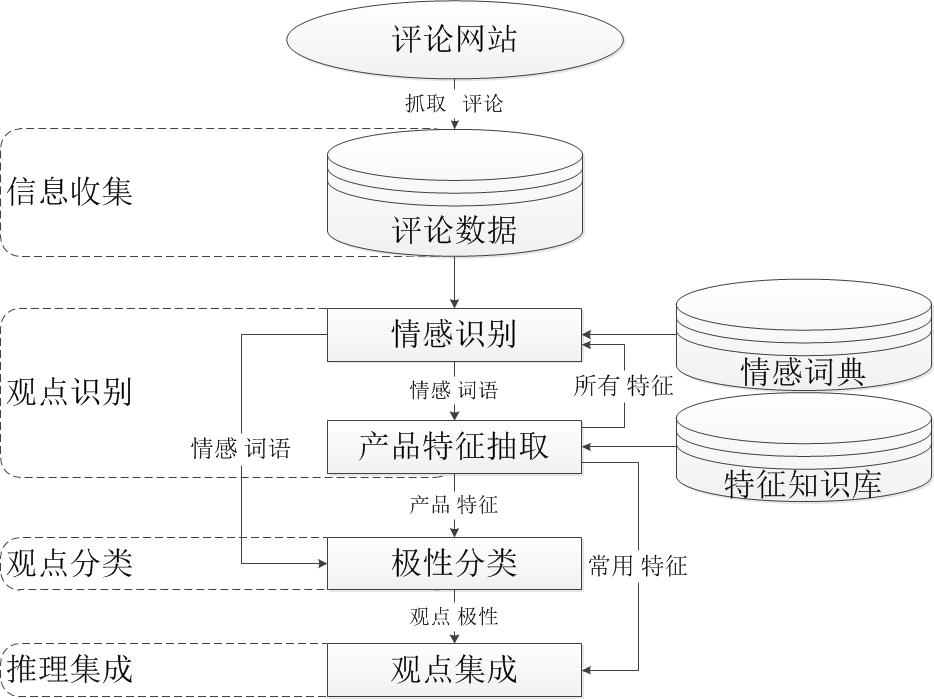
\includegraphics[height=220pt]{1-2.jpg}
\caption{产品评论的观点集成框架}
\label{fig1-2}
\end{figure}

对于文档集$ D $中的针对某话题的观点进行集成形式化表示为:
\begin{equation}
\{(f,s_f)|rep(f,D)>\rho_f,s_f=agg(S,f)\}
\end{equation}
其中$ f $表示根据某种表示度量方法$ rep(f,D) $确定的描述话题的不同方面,$ s_f $是针对$ f $根据集成函数$ agg(S,f) $计算出的针对$ f $的观点。

观点集成一个主要的挑战就是如何确定描述话题的多个不同方面。Leouski等\upcite{Leouski1996}评测了各种文本聚类方法对检索结果中信息的集成效果,发现聚类方法对于文本的交互式检索是有用的。Zeng等\upcite{Zeng2004}使用监督学习方法从文本中抽取主要短语并将其聚类表示话题的方面。越来越多的工作使用生成模型发现文档中的隐性方面话题\upcite{Su2006,Titov2008},还有一些工作使用数据挖掘中的联合规则方法对产品的相关方面进行挖掘\upcite{Liu2005,Popescu2007}。

\subsection{传播行为分析}
\label{rel3}
社交媒体中信息传播具有重要的应用价值,信息传播的主体是人,也就是社交网络的用户,研究人的传播行为是研究信息传播的重要组成部分。社交媒体中最具影响力的是微博上的信息传播,因为用户在微博的转发行为会使得信息在短时间内形成大规模的传播,因此本文主要从微博的转发行为来阐述相关工作。微博的典型代表是Twitter,Twitter转发机制,即重新发布其他人发布过的微博,以便于作者的全部粉丝看到转发的信息,使得信息迅速形成病毒式传播(viral propagation)。很多对于转发行为的研究分析涉及影响转发行为的因素,包括tweet的文本内容与转发的关系,用户的属性如何决定其他人的转发;Twitter中信息的一般传播路径与规律等等。

Boyd等人研究了Twitter中转发的各种类型以及转发的原因,他们分析了不同用户,用户属性,用户交流方式对于转发的影响,同时也分析了人们在Twitter中喜欢转发的内容\upcite{boyd2010tweet}。他们发现18\%的转发tweet包含hashtag,52\%的转发tweet包含链接,11\%的转发tweet包含连续的转发符号串(如,“RT @user1 RT @user2 ”),另外,9\%的转发tweet都包含回复原tweet作者的回复字符串(“@reply”)。这说明tweet文本中的hashtag,链接、回复、提交和转发符号都与tweet的转发存在着一定的对应关系。

Yang和Counts通过Twitter中的提及(“@username”)抽取了用户之间的关系,并在此基础上构造了用户关系的复杂网络。他们研究了信息在这个复杂网络上是如何传播的,包括信息传播的速度,规模,以及范围\upcite{yang2010understanding}。他们发现大约只有25\%的tweet是被信息作者的朋友转发,大部分是被粉丝但非朋友转发。这说明Twitter中用户形成的复杂网络,影响着人们的转发行为,因此信息在传播路径上具有一定的规律可循。

Macskassy和Michelson分析了一个月用户的Twitter数据,他们解释了各种信息传播的方式,尤其是转发的行为模式,他们发现tweet的内容是tweet被转发的决定因素,因此他们构建了基于内容的转发模型\upcite{Macskassy2011}。

Starbird等人对具体事件在Twitter上的传播进行了深入研究,他们分析了2011年埃及的政治事件,演示了这个事件的相关信息在Twitter上是如何生成,发展,传播的\upcite{starbird2012will}。

Comarela等人研究了影响用户回复或转发的因素,他们发现以前是否回复,发布信息的频率,信息的时效性,tweet的长度决定用户是否回复\upcite{comarela2012understanding}。

除了以上的工作,最新的研究还从不同角度对Twitter中的转发行为进行了深入的研究\upcite{kupavskii2013predicting,jenders2013analyzing,ahmed2013peek,bao2013popularity}。

综上所述,影响用户转发行为的因素主要包括tweet文本的内容、tweet文本的社交媒体属性(如是否包含链接、hashtag、提及等)、tweet作者的用户属性,tweet作者的朋友圈子,当然以上的研究都是从宏观上大规模分析Twitter转发数据得出的研究结论。从微观的角度则可以考虑给定一个tweet,未来这个tweet是否会被转发,是一个值得研究的问题。

虽然已有的Twitter转发研究从许多不同的角度进行了考虑,但是还没有工作从用户的主观动机角度进行研究,本文我们将结合用户观点分析研究的结果对转发行为进行分析。另外,目前的转发大多都是从tweet本身进行考虑,并未从受众的角度进行分析,本文将对tweet、作者、受众三个方面在转发过程中的相互关系进行探讨。

\section{研究内容与方法}

\subsection{本文研究内容}
本文的研究内容主要是围绕社交媒体上的观点信息的分析应用,从两个角度对用户产生的带有观点的内容进行建模:一个角度是从不规范的社交媒体文本中发现观点信息,并在用户层面进行观点集成对用户的主观性进行建模,另外一个角度是利用用户产生内容中分析得到的用户主观模型分析用户在使用社交媒体时的一些在线行为,本文主要分析用户在微博的转发行为。研究框架如图\ref{fig1-3}所示。

\begin{figure}[htp]
\centering
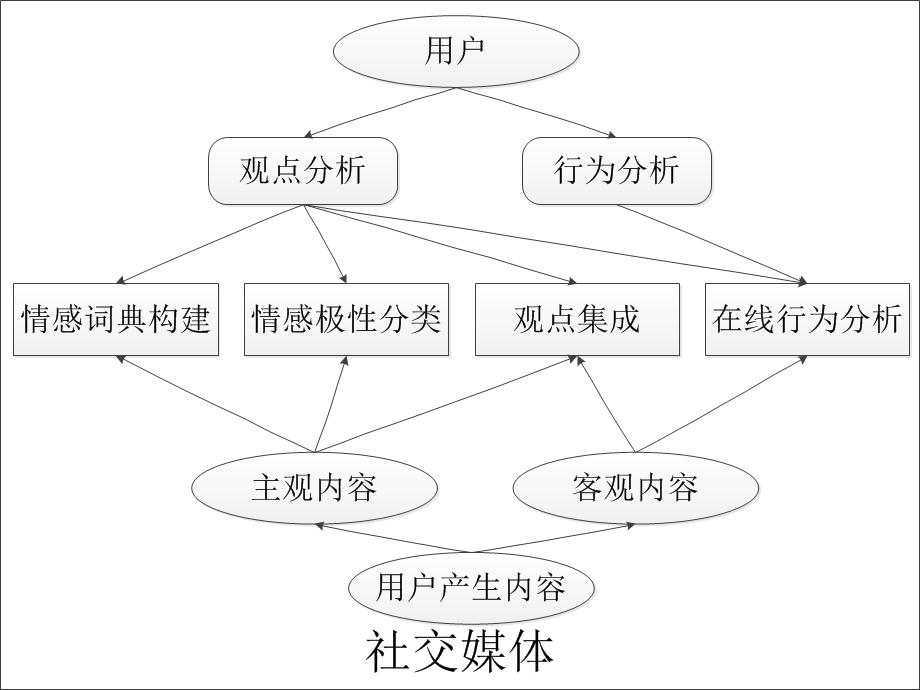
\includegraphics[height=230pt]{1-3.jpg}
\caption{本文研究框架}
\label{fig1-3}
\end{figure}

本文主要研究内容分为四个部分:首先从社交媒体文本中得到观点信息属于观点挖掘研究内容,观点挖掘方法分为基于情感词典和基于机器学习的方法,因此需要进行\textbf{情感词典的构建研究}以及判断观点极性的\textbf{情感分类研究};其次从社交媒体文本片段中挖掘到的观点需要进行整合集成,变成具有代表性的观点信息,属于观点集成的研究内容,我们将从用户维度对用户的所有观点进行集成,用于\textbf{用户主观性建模};最后利用用户的主观模型,从行为主观动机角度对用户的信息传播行为进行分析,属于\textbf{转发行为分析}研究内容。
具体四个研究内容的阐述如下:

\begin{enumerate}
\item \textbf{情感词典的构建}:使用已有的比较成熟的英文情感词典中的情感知识进行跨语言情感知识转移,构建一个通用的中文情感词典;针对通用情感词典领域适应性弱的问题,通过基于语料库情感词典扩展研究,使用语料中的语言特征以及统计特征,对情感词典在领域内进行扩展以增强情感词典的领域适应性。
\item \textbf{情感分类}:根据社交媒体情感表达方式的领域依赖性,对情感分类特征空间进行分割,将领域独立的通用特征与领域依赖特征分开,使用两部分特征分别训练分类器,通用分类器使用现成资源训练,领域分类器使用远监督方式训练,最后两个分类器在自举式机器学习框架下组合成性能更强的情感分类器。
\item \textbf{用户主观性建模}:提出一个通用的主观模型定义,将用户产生内容中关注的话题和针对这些话题表达的观点组合在一起,对用户在每个话题上发表的所有观点整合集成,并使用一个在情感极性值空间中的分布表示用户在话题上的综合观点,使用一个更简单通用的框架构建主观模型。
\item \textbf{转发行为分析}:构建好每个用户的主观模型后,给定微博,发现作者的粉丝中,谁会在未来传播微博,从用户的主观动机角度,分析用户在三种转发情形下的主观动机,即微博内容的吸引力,转发微博的社交需求以及转发微博的认同需求。
\end{enumerate}

总的来说,针对~\ref{point}的第一个问题,本文通过构建情感词典识别社交媒体中带有观点的文本信息,并使用无监督的情感分类方法对观点的极性进行分类;
针对~\ref{point}的第二个问题,本文通过将用户关注话题与发表的观点进行组合建模,采用集成的观点表示方式对用户的主观性进行建模;
针对~\ref{point}的第三个问题,本文通过计算主观模型之间的相似性度量用户一些在线行为的主观动机,进行行为的分析。

\subsection{本文研究方法}
社交媒体中的观点分析涉及到信息检索、机器学习、自然语言处理与自然语言理解等多方面的方法和技术,这些方法和技术的综合使用是由社交媒体数据特有的性质以及观点分析应用的特殊需求所决定的。
从社交媒体数据特性来看,进行观点分析需要面临以下挑战:
\begin{itemize}
\item 社交媒体中的文本篇幅较短而且噪声较多的特点,使得利用标准的机器学习方法进行分析面临数据稀疏问题,也造成自然语言处理技术的困难;
\item 庞大的数据容量以及动态的语言特性造成通用的标注数据的匮乏,无法满足机器学习训练要求;
\item 社交媒体是一个开放平台,文本涉各种领域,因此各种方法和技术都要满足多领域环境的需求;
\item 社交媒体中的数据以数据流的形式不断高速增长,需要能够快速适应新数据并实时处理的技术和方法。
\end{itemize}

观点分析需要从大量的社交媒体用户产生的内容中发现观点信息,进而进行整合集成并用于分析用户的转发行为,要解决以上问题和挑战,需要达到如下几个主要目标:
\begin{enumerate}
\item 使用文本规范化和消除噪音等自然语言处理技术对数据进行预处理,数据的稀疏性需要得到缓解,然后才能进入后面的分析中;
\item 观点极性分类方法应该具有领域独立能力,当领域变化时能够快速适应并且性能不能下降;
\item 采用的所有技术和方法能够以有限的计算能力分析和处理不断增长的数据;
\item 针对训练数据缺乏问题,尽量使用无监督或者弱监督的方法和技术,并且尽量使用已有的资源,减少人工标注。
\end{enumerate}  

针对以上挑战和目标,我们确定的研究方法为:

首先在数据和资源选择上,我们首要选择已有的知识资源和标注数据。如果没有对应的知识资源,可以通过资源转化变成我们想要的知识资源,比如情感词典构建时,我们通过情感知识之间的对应关系,将英文情感词典转化为中文情感词典。如果没有直接标注数据,我们选择采用弱标注的方法得到训练数据,所谓弱标注数据指的是,数据的类别标签是通过启发式从数据中直接确定不需要人工标注,比如在训练情感极性分类器时,我们使用含有明确情感极性的成语微博作为训练数据,是基于微博短小观点表达相对会集中在一些极性相同的词语身这一假设,从而获得大量训练数据。在理想的情况下,用弱标记数据的好处是双重的:首先,我们可以以接近零的代价采集训练数据,因此可以轻松地将我们的应用扩展到其他领域或语言。其次,弱标注语料的规模可以很容易超越常规手动标注的训练语料的数量级。

在学习训练方法的选择上,我们优先选择无监督或半监督的机器学习方法。无监督或办监督学习方法可以减少或无需大量的标注训练数据,而且可以通过迁移方法将学习到的知识进行跨领域或语言转换。比如我们在对微博进行极性分类时,使用自举式机器学习方法将两个弱的分类器结合在一起提高了分类的性能;在构建主观模型时,我们使用LDA话题模型识别用户关注的话题,并使用基于规则的情感分析方法获得用户的观点信息。  

\section{本文主要贡献}
本文以用户为单位,对用户在社交媒体上产生内容中的观点信息进行识别、分析和集成,并使用得到的观点信息分析用户在社交媒体上的在线交互行为,具体来说本文的主要贡献为:
\begin{itemize}
\item 设计了一种中文情感词典的自动构建方法,该方法能够从已有的英文情感词典通过词语之间的对应语义关系转化情感知识,并且能够针对任何领域的语料进行扩充,成为准确性更高的领域情感词典。通过与其他中文情感词典的对比,我们的情感词典完全是自动构建,而且具有更好扩展性和领域适应性。
\item 基于词语在表达情感时作用的不同,提出了一种新的无监督情感分类方法,该方法将情感分类的特征空间进行分割,在两个不同的特征空间分别训练分类器,然后以自举式学习框架组成更强的分类器。方法无需人工标注的训练数据,使用现有的成语词典资源和弱标注的远监督方法训练分类器,性能超过了需要大量标注数据训练的有监督分类器。
\item 提出了从用户维度进行集成的通用的观点集成方法,该方法将用户感兴趣话题以及在话题上的观点组合对用户主观性建模,并且该模型能够在更细粒度的情感空间中使用分布方式表示观点,使得用户的观点表示更准确,综合反映了用户在话题每个方面所表达的观点,将该模型应用到观点预测任务时,能显著提高观点预测的准确性。
\item 从主观动机角度对用户在Twitter上的转发行为进行了分析,利用用户的主观模型设计了一种新的计算主观相似性方法,对用户转发行为的三种情形使用主观相似性进行度量,在真实Twitter数据中的实验中验证了三种主观相似性度量与转发行为之间的相关性,并且作为有用特征预测转发行为的准确性超过了目前一些主要方法,通过结合其他影响因素,可以使预测性能得到显著提升。
\end{itemize}

\section{本文结构}
本文的研究工作主要围绕社交媒体观点信息分析与应用任务展开,我们可以将这两方面的工作分为以下几个主要部分:在观点分析方面,我们首先探讨了如何利用现有资源进行中文情感词典的自动构建,情感词典是观点信息识别和情感分类的基础;然后进一步探讨了如何结合社交媒体的文本特点对文本中表达的观点进行极性分类;最后对社交媒体中的观点信息以用户为维度进行整合集成,形成用户在其产生内容中表达的所有观点信息的主观模型。对分析得到的主观信息应用方面,我们从用户作为信息传播的主体角度,对用户转发行为的主观动机使用主观模型进行度量和分析。上述工作共分为七个章节,论文主体结构以及章节之间的关系如图~\ref{fig1-4}所示。,每个章节内容具体安排如下:

\begin{figure}[htp]
\centering
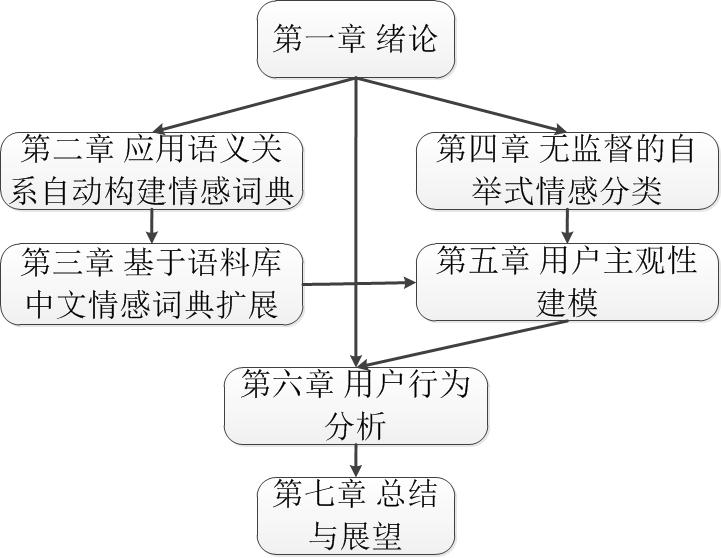
\includegraphics[height=250pt]{1-4.jpg}
\caption{论文整体结构图}
\label{fig1-4}
\end{figure}

第一章是绪论,首先介绍了本文研究的背景,介绍了社交媒体和观点分析一些基础知识,接着提出研究动机,阐明了本文所涉及的科学问题、研究内容,并给出了研究方法,然后分析了研究问题,确立了依托自然语言处理技术与机器学习方法解决这些问题的基本思路,最后介绍了本文的主要工作和文章的结构。

第二章是应用语义关系自动构建中文情感词典,首先介绍了目前情感词典资源的现状,针对中文情感词典资源缺乏问题,提出了以HowNet语义知识库为基础,根据中英文词典语义之间的对应关系将英文情感词典的情感知识转化到中文情感词典中,设计了转化方法以及转化中极性值的计算方法,实验中与现有的几个中文情感词典进行了对比。

第三章是基于语料资源的中文情感词典扩展,是对第一章中构建的通用情感在领域语料中的适应性扩展方法研究,首先介绍了基于语料资源的情感词典构建方法,确定了基于语言特征以及统计特征的扩展方法,并提出了综合使用两种特征的混合特征扩展方法,并分别进行了实验验证。

第四章是无监督的自举式情感分类,本章首先介绍了目前情感分类研究现状,针对领域依赖问题,根据词语在表达情感的不同作用提出了特征空间划分方案,并对研究问题进行了形式化,设计了自举式情感分类框架,选用了三种分类器并进行了实验对比分析。

第五章用户主观性建模,首先定义了社交媒体中用户的观点集成问题,然后提出了主观模型的框架,将用户产生内容中的话题和观点组合进行用户观点集成,并设计了通用的模型构建方法,实验中将主观模型应用到观点预测任务,并对模型进行了定性的分析。

第六章用户的转发行为分析,研究的问题是对于给定一个微博,分析微博作者的粉丝中谁会转发该消息,针对该问题,我们使用主观模型从用户的主观动机角度进行分析,设计了主观相似性计算方法,并针对转发行为的三种情形进行度量,最后在实验中定性和定量验证了我们提出方法的有效性。

最后一章是总结部分,我们阐明了本文工作的贡献点,并且指出了工作的一些不足,并对未来社交媒体中观点信息分析与应用的一些问题和方法进行了尝试性地思考。



\chapter{应用语义关系自动构建情感词典}
\label{ch2}
%本章将进入论文排版的正文, 按元素分主要包括:
%{\kai 字体段落,图片表格,公式定理,参考文献}这几部分。
%这个样例文件将包括模板中使用到的所有格式、模板中自定义命令到或者特有的东西,
%都将被一一介绍,希望大家在排版自己的学位论文前能细致的看一遍,记住样例的格式和
%方法,方便上手。

\section{引言}
\label{ch2:intro}
上一章主要介绍了本文的研究背景,要研究的科学问题,研究内容与方法,并指出观点分析一项基础的工作就是研究如何针对不同应用构建具有足够覆盖面并且良好适应性的情感知识词典。人在使用语言表达情感或观点时,最基本的方式是使用具有明确情感色彩的词汇,因此为了分析用户的观点,最直接的方法应该从用户产生文本中使用的词语开始,将语言中经常使用的词语所表达的情感信息进行汇总形成的词典就是情感词典。观点分析研究首先是在英文文本上开始的,情感词典相关研究也是以英文为主,方法相对比较成熟,形成了一些经常使用的英文情感词典资源。中文情感分析研究起步较晚,缺乏普遍认可的可靠的中文情感词典\upcite{朱嫣岚2006,朱征宇2013,黄硕2013}。目前研究使用主要有HowNet情感词典\upcite{2013},NTUSD情感词典\upcite{Ku2007}以及大连理工大学的情感词汇本体词库\upcite{2013a}。这些词典主要是以手工或半自动方式编辑而成,覆盖度、可靠性和领域适应性受到限制,并且情感知识主要以积极和消极极性二值区分,缺少情感极性值的细粒度划分。能够将资源丰富的英文词典中的情感知识跨语言向中文词典进行适应性的转化,构建相应的中文情感词典资源,既可以省去耗费大量人力的人工标注过程,又可以克服目前中文情感词典自动或半自动构建方法的可靠性和覆盖度问题。
因此本章提出将英文情感词典资源情感知识转化为中文情感词典的构建方法,可以根据语义关系将英文词语及其情感极性值转化得到中文词语的情感极性值,并且完全是自动的,可靠性更高。下一章将该方法构建的情感词典在领域语料中进行扩展,以提高其领域覆盖度和适应性。

本章具体安排如下:首先对情感词典构建需要考虑的问题以及相关工作进行全面的介绍,接着对本章要使用的词典资源进行介绍,然后详细阐述如何利用HowNet双语语义知识库将英文情感词典情感知识转化为中文情感词典相应的词语情感信息,最后对该方法进行实验验证和说明。

\section{相关工作}
构建情感词典需要考虑词典覆盖度(Coverage)、词典内容(Content)以及构建方法(Acquisition)三个方面问题,具体内容可以用图~\ref{fig2-1-1}框架来展示。

\begin{figure}[htp]
\centering
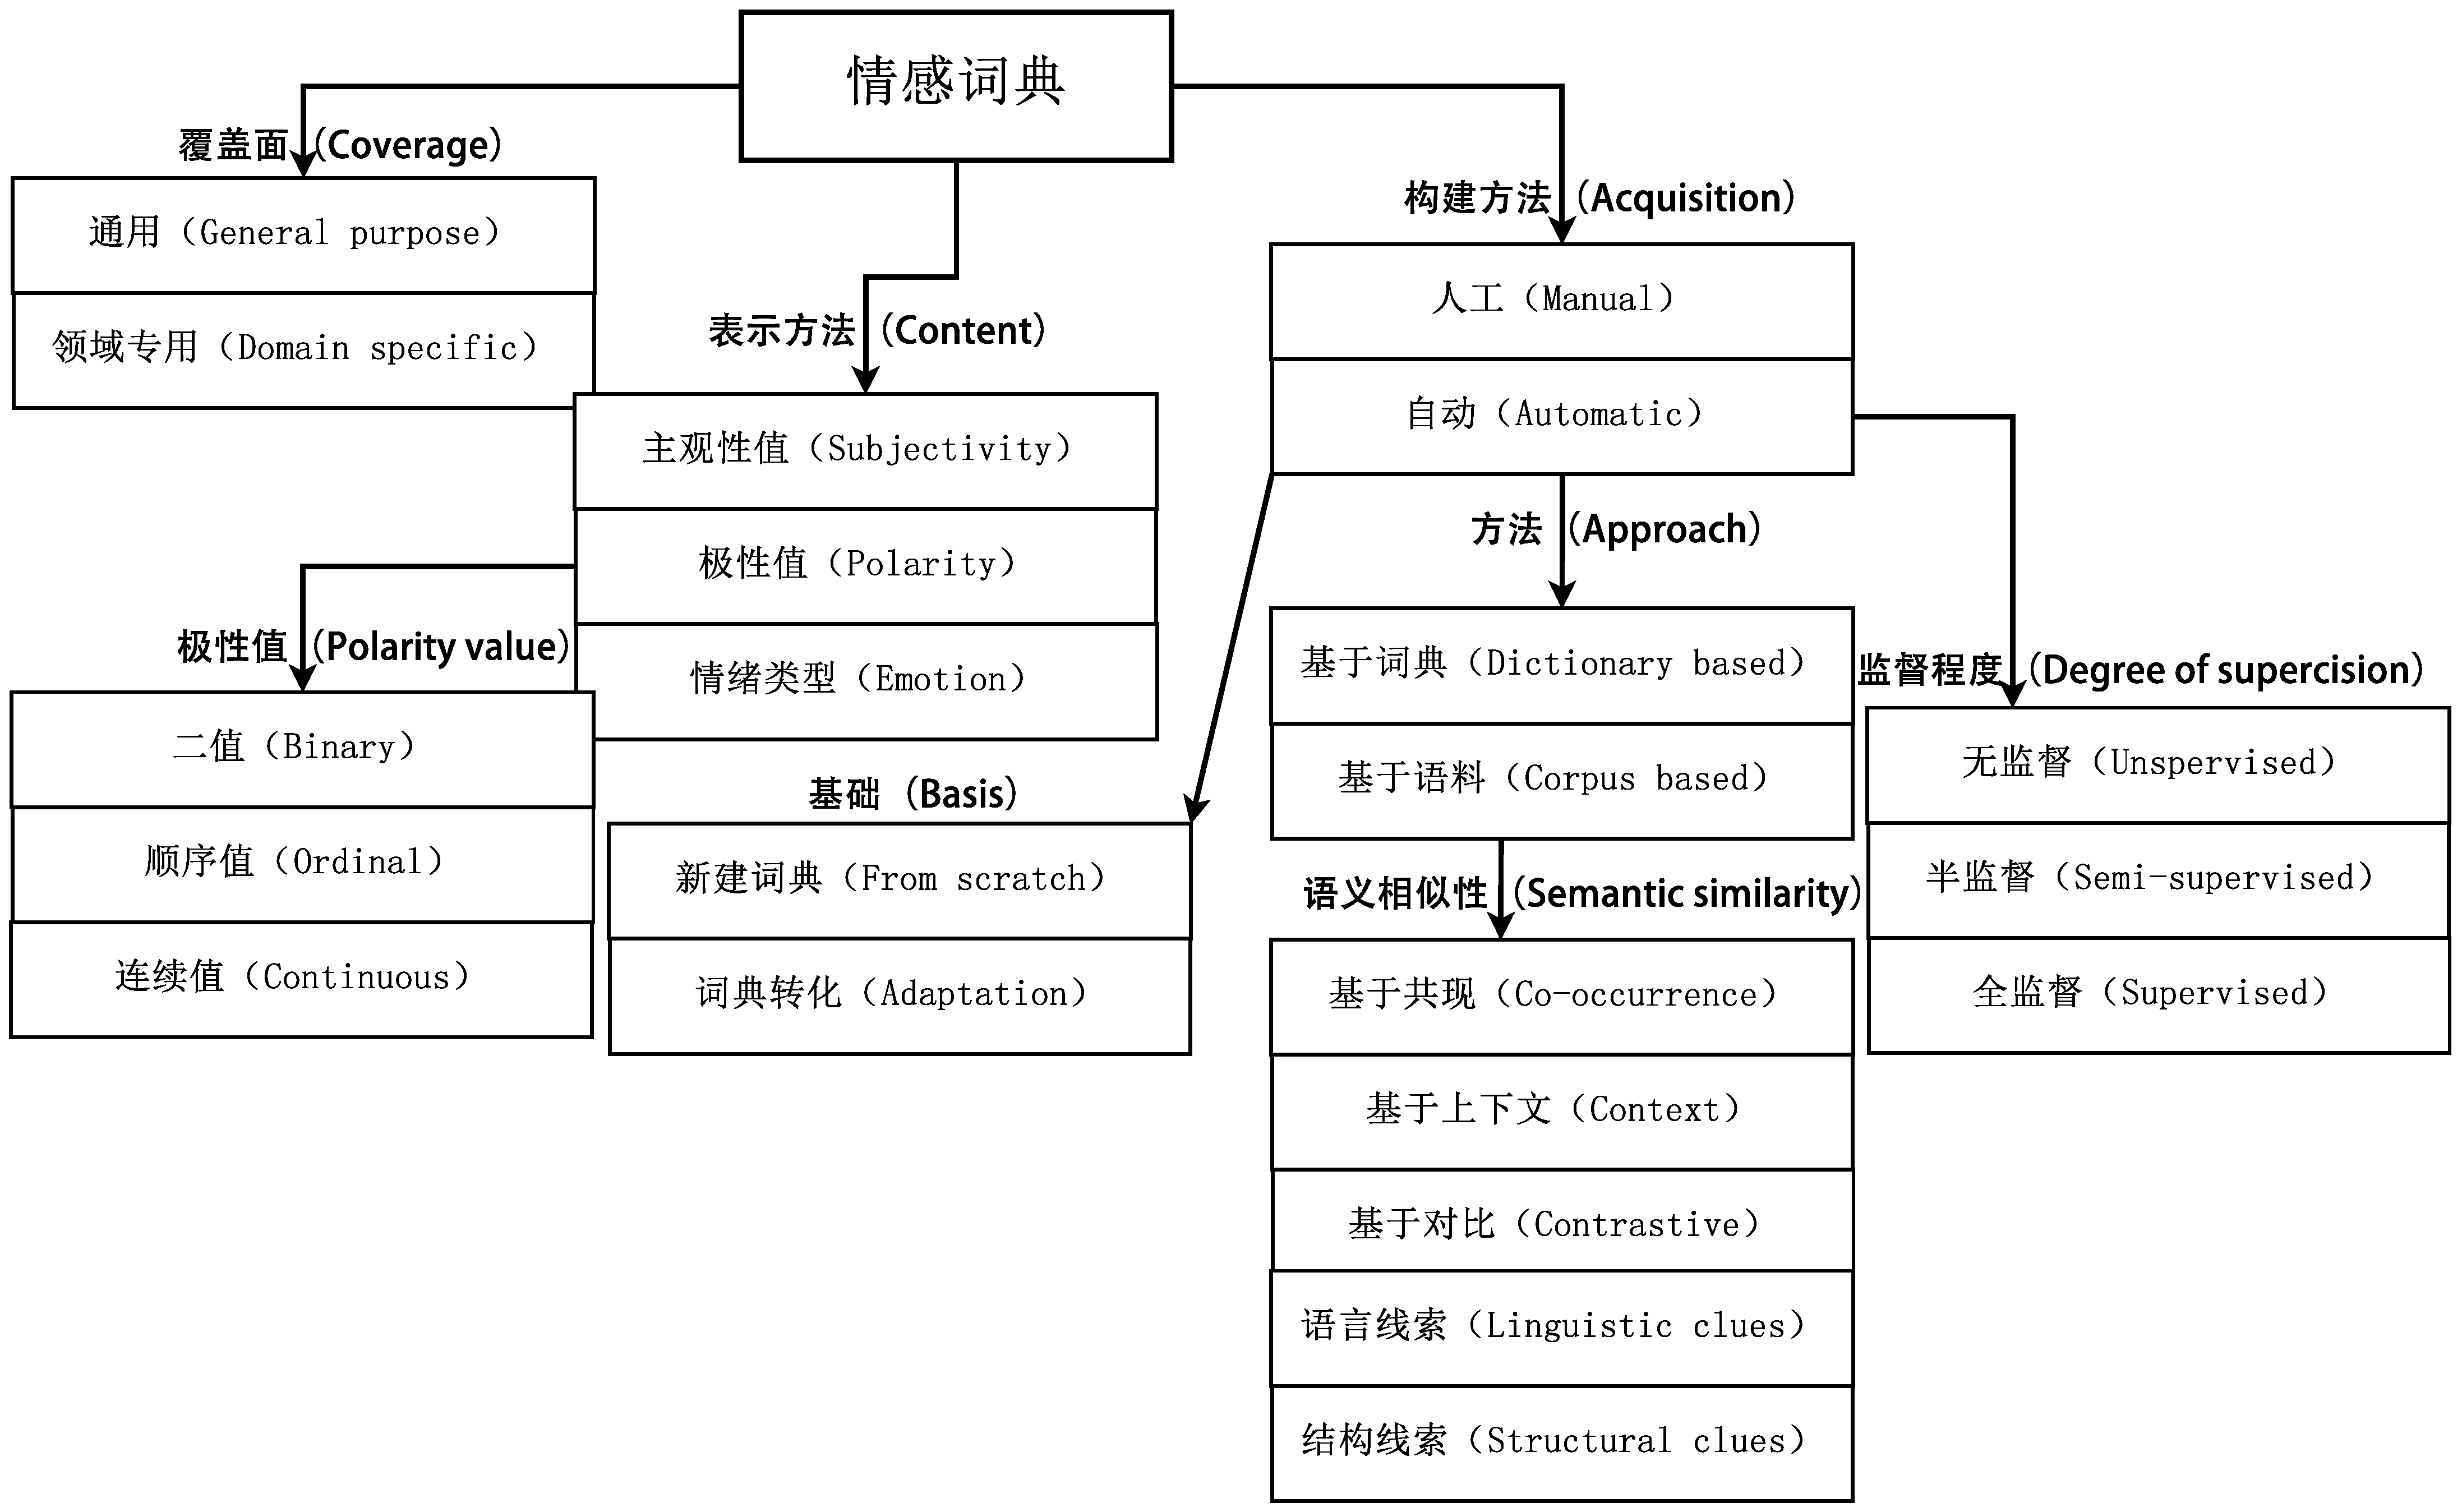
\includegraphics[height=300pt]{2-1-1.eps}
\caption{情感词典相关研究}
\label{fig2-1-1}
\end{figure}

\subsection{词典覆盖面}
就词典的覆盖面来讲,情感词典可以分为通用词典以及领域专用词典。构建通用情感词典的主要假设就是希望词语表达的情感独立于具体的领域和应用,当然这一假设只对一部分词语(比如:“赞”、“爱”、“憎恨”等)是合理的,目前经常使用的情感词典基本都是通用的情感词典。但是实际上很多词语表达的情感是依赖于领域和具体的语境的,比如“轻薄”一词,一般情况表示负面情感,但是描述手机时却可以表示正面的评价。而且,一些本身不表示具体情感的词语(比如:“长”、“短”、“老”、“经典”等),用到一些特殊的语境时也会表达出一些具体情感(比如:“手机待机时间长”与“手机待机时间短”)。因此一些研究开始针对具体领域和应用需求构建一些领域专用的情感词典\upcite{Choi2009,Du2010,Klenner2009}。

\subsection{词典内容}
情感词典可以就其表示情感知识内容进行细分,如果不考虑具体的应用场景,仅对词典的情感表示方法进行划分,情感词典表示情感知识的方法可以分为三种:词语表示主观性的程度(Degree of subjectivity)、表示情感的极性(Polarity)或者表示的情绪类型(Emotion$ / $mood,比如喜、怒、哀、乐等)。表示主观性程度的情感词典主要用于文本主观性的探测任务\upcite{CarmenBanea2008,Gyamfi2009,Maks2012,Wiebe2000,Wiebe2006},而主观文本表达观点的具体情感类型的识别,需要表示情感极性或情绪类型的情感词典。在情感分类中经常使用是表示情感极性的词典,词典中词语条目都标注了表达的情感极性是积极的还是消极的,这些极性知识对于确定文本所表达观点的倾向性是非常重要的。对这类情感词典还可以根据表示的情感极性值进一步划分:比如使用二值情感极性(也就是积极的和消极的)的情感词典\upcite{Godbole2007,Hatzivassiloglou1997,Hu2004,Rao2009};使用顺序值(ordinal)表示极性值的情感词典,比如常使用1-5整数值区分情感极性的强度值\upcite{Yessenalina2011};还有一些使用连续数值(continuous)表示情感极性强度的情感词典\upcite{Turney2003,Sasha2008,Velikovich2010,Remus2010}。
目前有很多这样的英文情感词典,比如:OpinionFinder(OF)\upcite{Wilson2005d},Appraisal Lexicon(AL)\upcite{Taboada2004},SentimentWordNet\upcite{Baccianella2010}以及Q-WordNet\upcite{Agerri2010}等。

如果为了分析更细粒度(fine-grained)的情感,需要将词语表达的情感根据情绪类型进行表示,比如Bollen等\upcite{bollen2011twitter}通过分析Twitter中大量用户表达出的不同情绪来预测股票指数的变化,Garcia和Schweitzer\upcite{Garcia2011}对产品评论中的情绪类型进行了细致研究,类似的工作还有Davidov等\upcite{Davidov2010}以及Strapparava和Mihalcea\upcite{Strapparava2008}在Twitter上的工作。这种类型的情感词典都是靠人工编辑形成的,比如GI(General Inquirer)\footnote{\url{http://www.wjh.harvard.edu/~inquirer/Home.html}}\upcite{Stone1966},ANEW(Affective Norms for English Words)upcite{Bradley1999},WordNet-Affect\footnote{\url{http://wndomains.fbk.eu/wnaffect.html}}upcite{Valitutti2004,Valitutti2004a},DAL (Dictionary of Affect in Language)\upcite{Whissell1989}等词典。

\subsection{词典构建方法}
从情感词典的构建方法来看,可以分为人工构建和自动构建两种类型。目前公开可用的人工编辑的情感词典基本都是通用的情感词典(比如:OF词典和GI词典),人工构建情感词典主要面临的问题除了需要耗费大量的人力,还有覆盖面相对较低,并且需要对不同的领域进行适应性扩展才能达到好的观点分析效果。
对于自动构建情感词典方法,还可以按照方法(Approach)、监督程度(Degree of supervision)和构建基础(Basis)三个维度进行区分。

\subsubsection{构建方法}
情感词典主要的构建方法分为两类:一是基于词典(dictionary-based)方法,根据已有词典的词语之间的语义关系判断词语的情感极性并计算情感极性值;二是基于语料(corpus-based)方法,根据词语在语料中的分布特性推导出情感极性并计算极性值。两类方法共同特点是都需要一个预先标注的种子词集(seed set),然后通过不断迭代计算词语与种子词集词语之间的某种语义相似性,推导词语情感极性值并扩充种子词集,直到收敛。

\paragraph{基于词典方法:}
基于词典的方法通常会使用一个词库(thesaurus)或语义知识库(常用的是WordNet\upcite{Miller1995}),基本的假设是词语间的语义关系可以用来确定词语的情感极性,最常用的语义关系是词语间的同义和反义关系\upcite{Godbole2007,Kim2006,Ahsaee2010}。例如形容词“lovely”会将积极极性通过同义关系传递给“admirable”、“adorable”、“amiable”和“pretty”,反过来会将消极极性传递给反义词语“awful”、“unlovely”和“ugly”。但是这种转换会随着语义距离增加而弱化,比如在WordNet中从“good”到“bad”的同义关系距离长度只有3\upcite{Godbole2007},因此方法设计时需要采取适当措施将语义距离考虑在内\upcite{Godbole2007,Ide2006,Budanitsky2001,Kim2006,Ahsaee2010}。除了同义和反义关系,一些研究提出使用WordNet中的其他语义关系,比如“similarity”,“derived-from”,“pertains-to”,“also-see”或“attribute”等关系\upcite{Esuli2006,Valitutti2004a}。Takamura等\upcite{Takamura2005}以及Andreevskaia等\upcite{Andreevskaia2006}使用了并不直观的下位关系(hyponymy)构建情感词典。还有一些方法通过计算词语在词典中解释的相似性来度量词语间的语义相关性,然后根据这种语义相关性构建情感词典\upcite{Esuli2006,Baccianella2010,Takamura2007}。

\paragraph{基于语料方法:}
和基于词典方法一样,基于语料方法一个基本思想就是通过某种方法度量词语间的语义相关性,然后从带有情感极性标注的种子词集中推导出词语的情感极性。主要度量方法可以分为以下四种:
\begin{itemize}
\item \textbf{基于词语共现方法}:代表性的工作是Turney等\upcite{Turney2002,Turney2003},主要是假设“一个词语的语义倾向性(semantic orientation)\footnote{Turney使用语义倾向性指代词语的情感极性}往往与其共现的词语的语义倾向性相关”,因此他们使用点互信息PMI统计值对词语和种子词集的相关性进行度量,进而推导出词语的情感极性。
\item \textbf{基于上下文方法}:除了直接通过共现来度量两个词语的相关性,在统计语义学还有还有一种常用的方法就是使用词语的上下文信息。在Firth的《Contextual Theory of Meaning》一书中,提出一个基本的假设就是“a word is characterized by the company it keeps”\upcite{Firth1957},指出词语的语义信息是与上下文语境紧密相关的。一些基于语料的情感词典构建方法利用这一假设,提出在相似上下文出现的词语具有相同的情感极性,因此可以从情感极性已知的种子词集推导出上下文信息相同的词语情感极性\upcite{Baron2003,Wiebe2000,Velikovich2010}。
\item \textbf{基于对比方法}:该类方法将词语在前景(foreground)语料和背景(background)语料中的分布特点对比分析,从而进行情感词语的抽取构建情感词典。比如Maks和Vossen\upcite{Maks2012}研究了对数似然和相对频率比抽取情感词构建语情感词典,他们使用报纸新闻以及新闻评论作为主观前景语料,维基百科文本作为客观背景语料。相似的工作还有Stepinski和Mittal\upcite{Stepinski2007}。
\item \textbf{基于语言线索}:前面几种方法单纯依靠语料中统计出的信息,不考虑对文本的深层次语言学特性分析。一些工作认为一些常用的语言模式有助于词语的情感信息的探测。Hatzivassiloglou和McKeown\upcite{Hatzivassiloglou1997}发现一个句子中连词(“and”和“but”)对所连接词语的情感极性具有一定的限制作用,例如出现在“and”两边的词语一般具有相同的极性,而出现在“but”两边的词语一般极性相反,他们利用这种语言规则上的限制从文本语料中抽取并构建情感词典。在产品评论的观点挖掘研究中一些工作扩展了这种基于连词的语言规则,同时考虑句子内和跨句子的连词规则\upcite{Ding2008,Angel,Kanayama2006,Popescu2007}。
\item \textbf{基于结构线索}:代表性的工作是Kaji和Kitsuregawa\upcite{Kaji2006,Kaji2007}的工作,他们利用HTML文档中的结构线索分别抽取情感极性为积极和消极的句子集,从大量HTML文档中抽取出大概500,000主观句子用于训练情感分类器并构建情感词典。
\end{itemize}

\subsection{词典转化}
上述的所有情感词典构建方法都是从零开始(from scratch)构建新的情感词典,最近也有一些方法研究对已有情感词典进行转化,主要是增强通用情感词典的领域适应性或者从单语言情感词典扩展到多语言。通用情感词典进行领域转化方法,主要有Choi和Cardie\upcite{Choi2009}提出的基于线性规划方法,Du等\upcite{Du2010}提出的基于信息理论框架扩展方法以及Qiu等\upcite{Qiu2009}使用语言模式的扩展方法等。Mihalcea等\upcite{Mihalcea2007}提出了基于词典和基于语料的方法将英文情感词典通过翻译转化为其他语言的情感词典。

\subsection{混合方法}
混合方法指的是构建情感词典时同时考虑多种词典和语料资源。例如Hoang等\upcite{Hoang2008}提出使用WordNet的语义关系产生初始情感词典,然后使用从网络语料中获取的统计信息对其进行完善,词典资源和语料资源用一个误差最小化算法(error minimization algorithm)结合起来。Lu等\upcite{Lu2011}提出将与词语相关四种信息组合起来确定情感极性,包括在通用情感词典中的信息,在词库(thesaurus)中的信息,以及在领域文档集中的语言线索和结构线索信息,这四种信息使用一个基于线性规划的优化框架结合起来确定词语的情感极性。

综上所述,目前有很多种构建情感词典方法,以针对英文资源的构建方法研究为主。中文情感词典的构建方法研究还相对较少,基本上是借鉴英文的构建方法,形成的中文情感词典表示的情感知识是简单的二值极性。本章主要研究如何从英文词典进行转化得到中文情感词典,属于词典转化方法,具体的实现方法是借助于双语语义知识库中的语义关系实现这种转化,而不是使用翻译的方式,形成的情感词典能够通过计算将英文情感词典的情感极性值同时转化为中文情感词典的极性值,情感知识更加丰富。

%随着互联网的发展,尤其是社交网络的发展,各种社交媒体的用户发布内容中出现了海量含有用户主观情感色彩的文本数据。针对网络文本的信息处理开始由获得关键词\upcite{Yuan2013}、事件
%\upcite{张辉2013}、话题\upcite{刘健2013} 等事实信息,开始向情感观点等主观信息深入,情感分析便是近年来迅速发展的信息处理技术\upcite{Liu2012}。从数据中提炼出用户的主观信息对于商业情报、舆情分析等具有重要意义。情感分析技术就是对带有情感色彩的主观性文本进行自动推理、分析、归纳的过程,涉及自然语言处理、机器学习、认知科学以及社会心理学等方面的研究\upcite{黄萱菁2011}。


\section{词典资源简介}
\label{ch2:lex}
本节简要介绍要用到的一些词典和知识库资源,主要是针对本章研究相关部分作介绍。
\subsection{HowNet语义知识库}
HowNet是一个以中英文词语所代表的概念为描述对象,揭示概念与概念之间以及概念的属性与属性之间的关系的知识库\upcite{杜飞龙2000}。HowNet两个重要名词是“义原”和“概念”:概念是对词汇语义的一种描述,每一个词可以表达为几个概念\upcite{刘群2002};义原是最小语义单元,用于定义和描述概念。
\subsubsection{义原} 
HowNet设计了大概2200多个义原,这些义原分为几个大类,具体参见表~\ref{tab2-1}。

\begin{table}[htp]
\centering
\caption{HowNet义原分类}
\label{tab2-1}
\begin{threeparttable}
 \begin{tabular}{|l|l|l|l|}
 \hline
 义原&数量& 示例&语义倾向性\tnote{1}\\
 \hline
 Event$ | $事件& 819& blame$ | $埋怨& 一般有倾向性\\
 \hline
Entity$ | $实体& 142& human$ | $人 & 不具倾向性\\
\hline
Attribute$ | $属性& 117 & length$ | $长度 &一般不具倾向性\\
\hline
aValue$ | $属性值& 899 & good$ | $好 &一般有倾向性\\
\hline
Quantity$ | $数量& 3 & rate$ | $比率 & 一般不具倾向性\\
\hline
qValue$ | $数量值& 13 & ufficient$ | $足 & 一般有倾向性\\
\hline
SecondaryFeature$ | $次要特征& 100 & desired$ | $良&一般有倾向性\\
\hline
Semanticroles$ | $语义角色& 90 & StateFin$ | $终状态 & 一般不具倾向性\tnote{2}\\
 \hline
\end{tabular}
\begin{tablenotes}
%  \centering
  \footnotesize
\item[1]语义倾向性即情感极性。
\item[2]虽然语义角色类不具有倾向性,但是代表的语义关系可以影响其他义原的倾向性。
\end{tablenotes}
\end{threeparttable}
\end{table}

表中可以看出,除了事物类、属性类以及数量类义原,其他义原一般都具有情感极性,并且义原都是由中英双语标识,因此可以通过英文标识从英文情感词典中获得其情感极性值。但是有一部分义原的英文标识不是一个单词(比如:FondOf$ | $喜欢,WhileAway$ | $消闲等),无法直接从英文情感词典直接获得情感极性值。实际上义原之间并不是独立的,义原之间存在复杂的关系,HowNet中描述了义原之间的主要的8种关系:上下位关系、同义关系、反义关系、对义关系、属性-宿主关系、部件-整体关系、材料-成品关系、事件-角色关系。义原之间组成的是一个复杂的网状结构,而不是一个简单树状结构。不过,义原关系中最重要关系是上下位关系,义原根据上下位关系形成了如图\ref{fig2-2}树状层次体系,因此可以借助上下位关系树对无法直接转化那部分义原的情感极性值的计算。

\begin{figure}[htp]
\centering
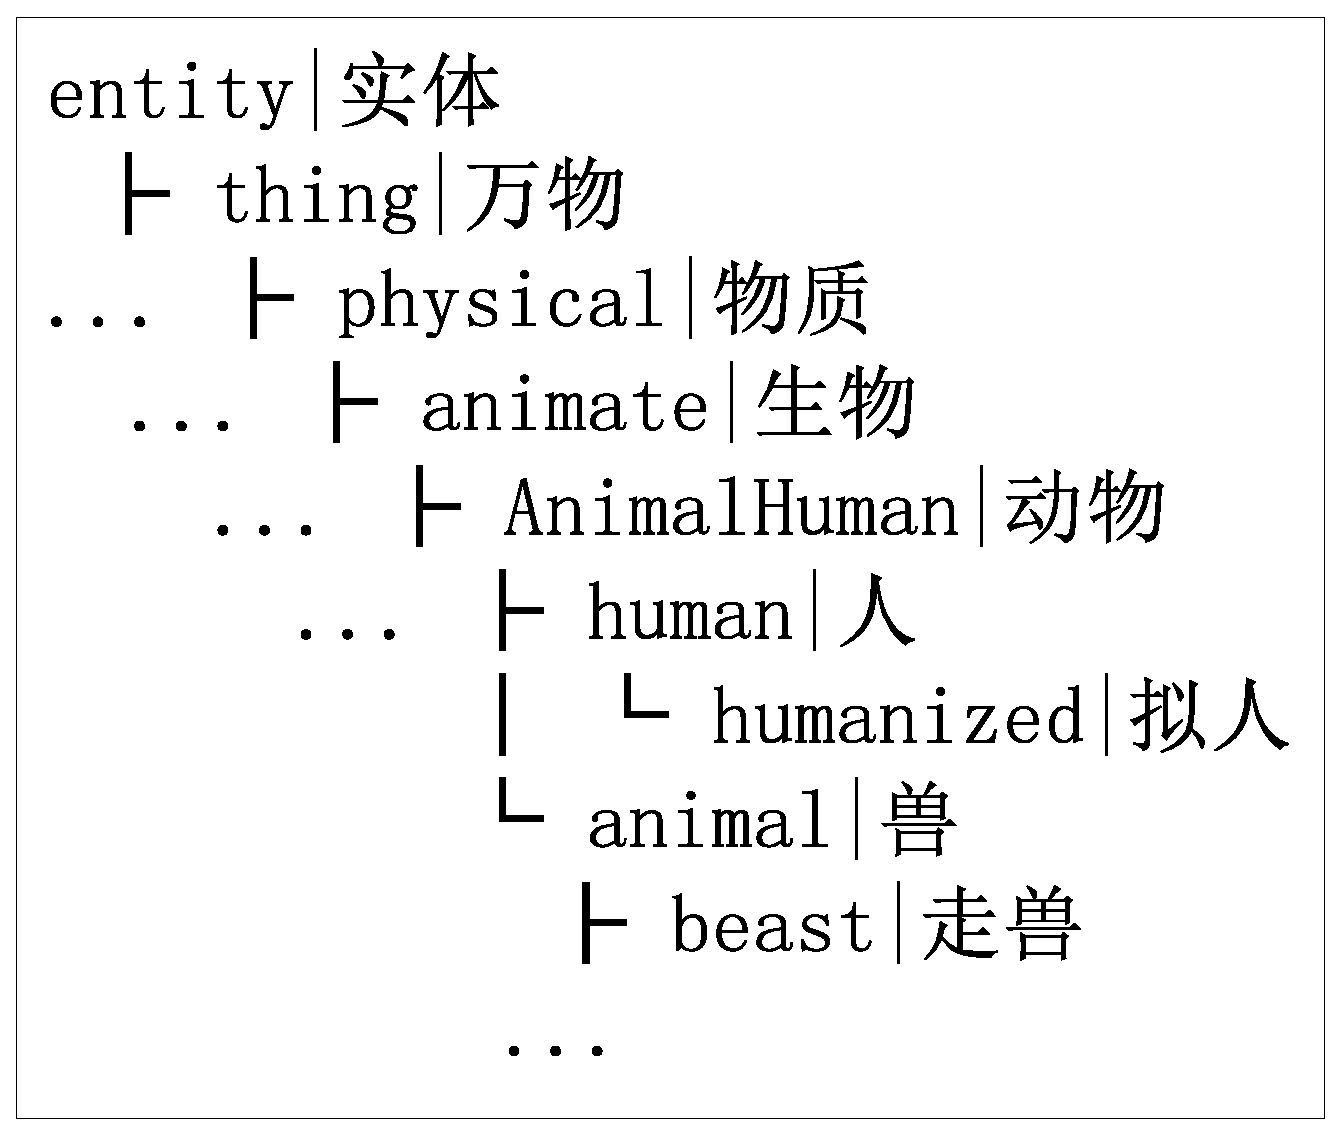
\includegraphics[height=160pt]{2-1-0.eps}
\caption{HowNet义原层次结构}
\label{fig2-2}
\end{figure}

除了义原以外,HowNet还有一些符号(或称为符号义原)对概念语义描述,可以把这些符号归为几类:第一类包括“$ , $”(表示“和”的关系)、“$\sim $”(表示“或”的关系)、“$ \wedge$”(表示“非”的关系),用来表示语义描述式之间的逻辑关系;第二类包括“$\#, \%, \$, \& ,\ast,+,?,!,@ $”,表示概念之间以及概念的属性之间的关系;第三类包括几个无法归入以上两类的特殊符号“$\{\}, \left( \right), \left[ \right]$” 。这些符号义原中第一类描述逻辑关系的三个符号会引起所描述义原情感极性的变化,尤其是“$ \wedge$”会引起情感极性的反转。

\subsubsection{概念}
如图~\ref{fig2-3}所示,HowNet采用KDML(Knowledge Dictionary Mark-up Language)语言描述概念,其中W\_X表示词语,G\_X表示词语词性,E\_X表示词语例子,X为C时表示中文,X为E时表示英文。
%DEF是对于该概念的定义项,称之为一个语义表达式,其中中英文标注的是义原,“\#\*”等标示符号来对概念属性之间关系进行描述,DEF中还可以包含概念,概念之间相互交织构成一个网。HowNet一共有2234个义原,收录了近15万条概念记录,涵盖了绝大部分中文常用词语,本章将基于HowNet的词语进行情感词典的构建。

\begin{figure}[htp]
\centering
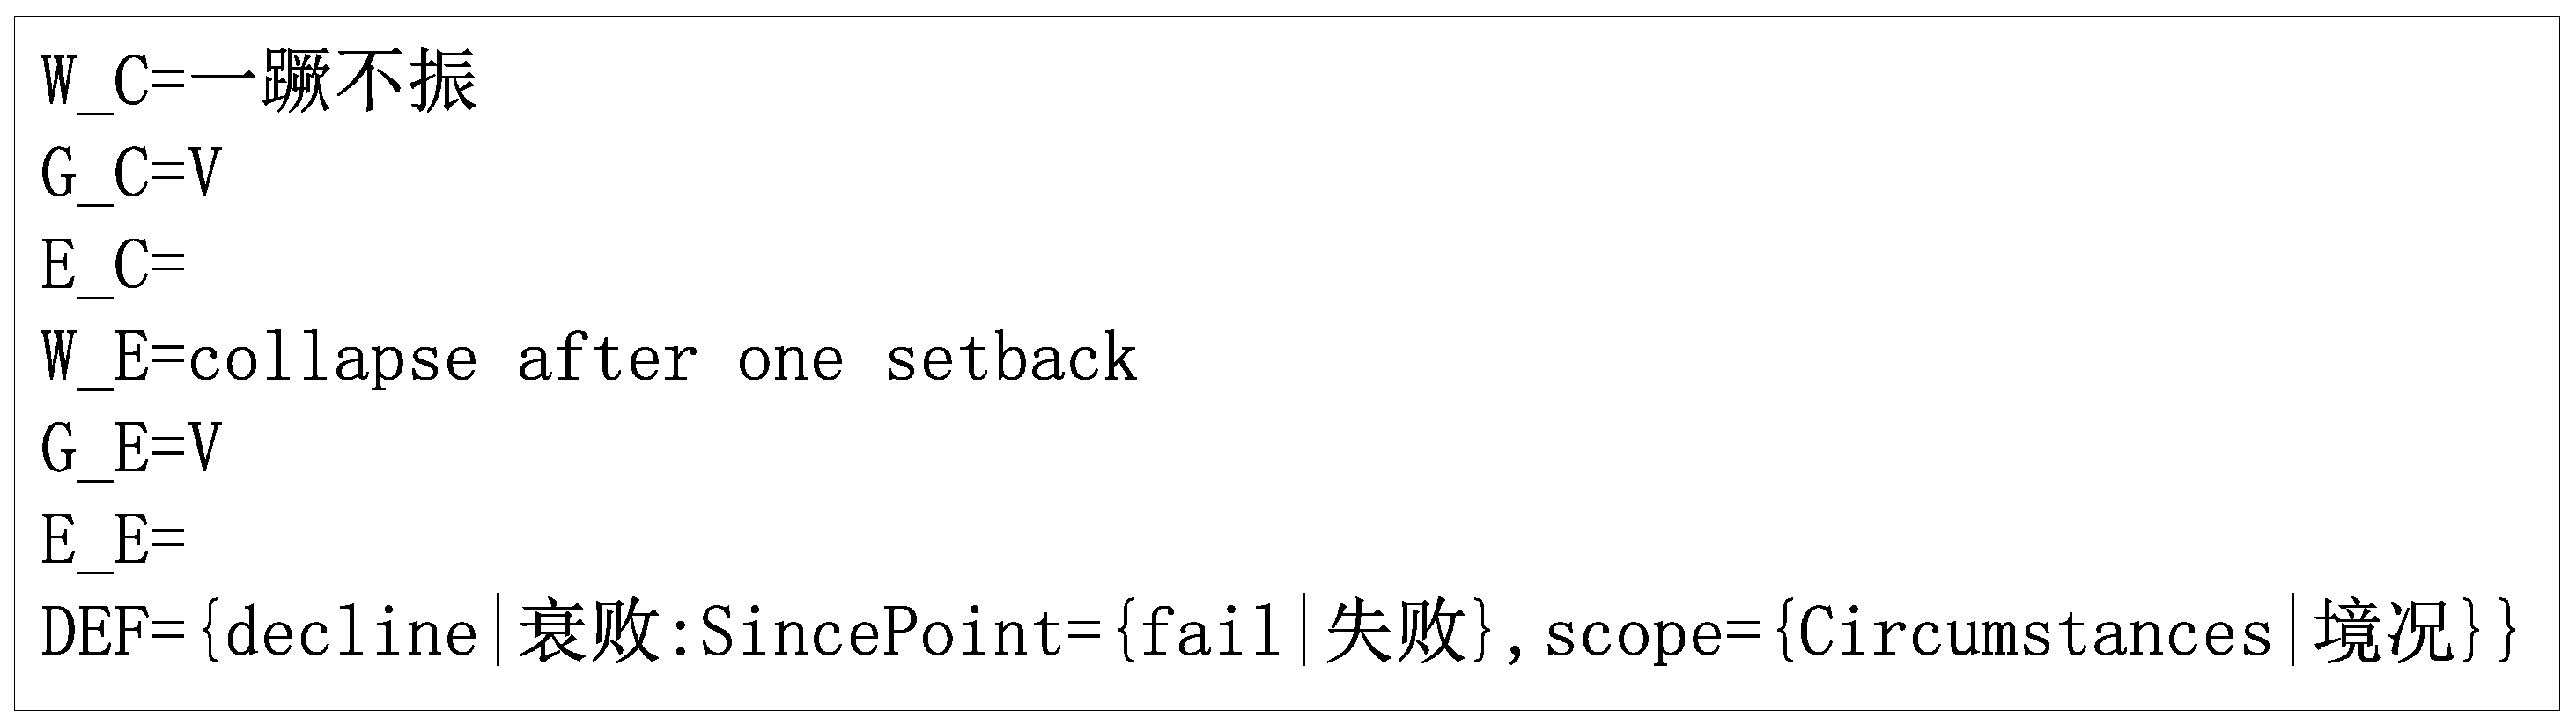
\includegraphics[height=120pt]{2-1-2.eps}
\caption{HowNet中概念描述方式}
\label{fig2-3}
\end{figure}
DEF是HowNet对于概念的定义,称为语义表达式,是知网的核心。HowNet知识描述语言是比较复杂的,为了后续分析计算,在此归纳为以下几条:
\begin{enumerate}
\item HowNet收录词语主有两类,即实词和虚词;
\item 虚词描述比较简单,用“\{句法义原\}”或“\{关系义原\}”进行描述,虚词不具情感极性;
\item 实词的描述就比较复杂了,由一系列用逗号隔开的语义描述式组成,其中语义描述式分为三种形式:
     \begin{enumerate}
     \item 独立义原描述式:用“基本义原”,或“(具体词)”描述;
     \item 关系义原描述式:用“关系义原=基本义原”,或“关系义原=(具体词)”,或“(关系义原=具体词)”描述;
     \item 符号义原描述式:用“关系符号 基本义原”或者“关系符号(具体词)”加以描述;
     \end{enumerate}
\item 实词描述代表了该词的语义知识,因为实词一般具有语义倾向性,因此实词的描述式可以帮助确定语义倾向性。
\end{enumerate}

\subsection{WordNet语义词典}
WordNet是由Princeton大学的心理学家、语言学家和计算机工程师联合设计的一种基于认知语言学的英文词典\upcite{Fellbaum1998}。WordNet是根据词义而不是词形来组织词汇信息。如图~\ref{fig2-2-3}所示,WordNet使用同义词集合(Synset)代表概念,词汇关系在词语之间体现,语义关系在概念之间体现。WordNet将英语的名词、动词、形容词和副词组织为Synsets,每一个Synset表示一个基本的词汇概念,并在这些概念之间建立了包括同义关系(synonymy)、反义关系(antonymy)等多种语义关系,其中最重要的关系就是词的同义反义关系。

\begin{figure}[htp]
\centering
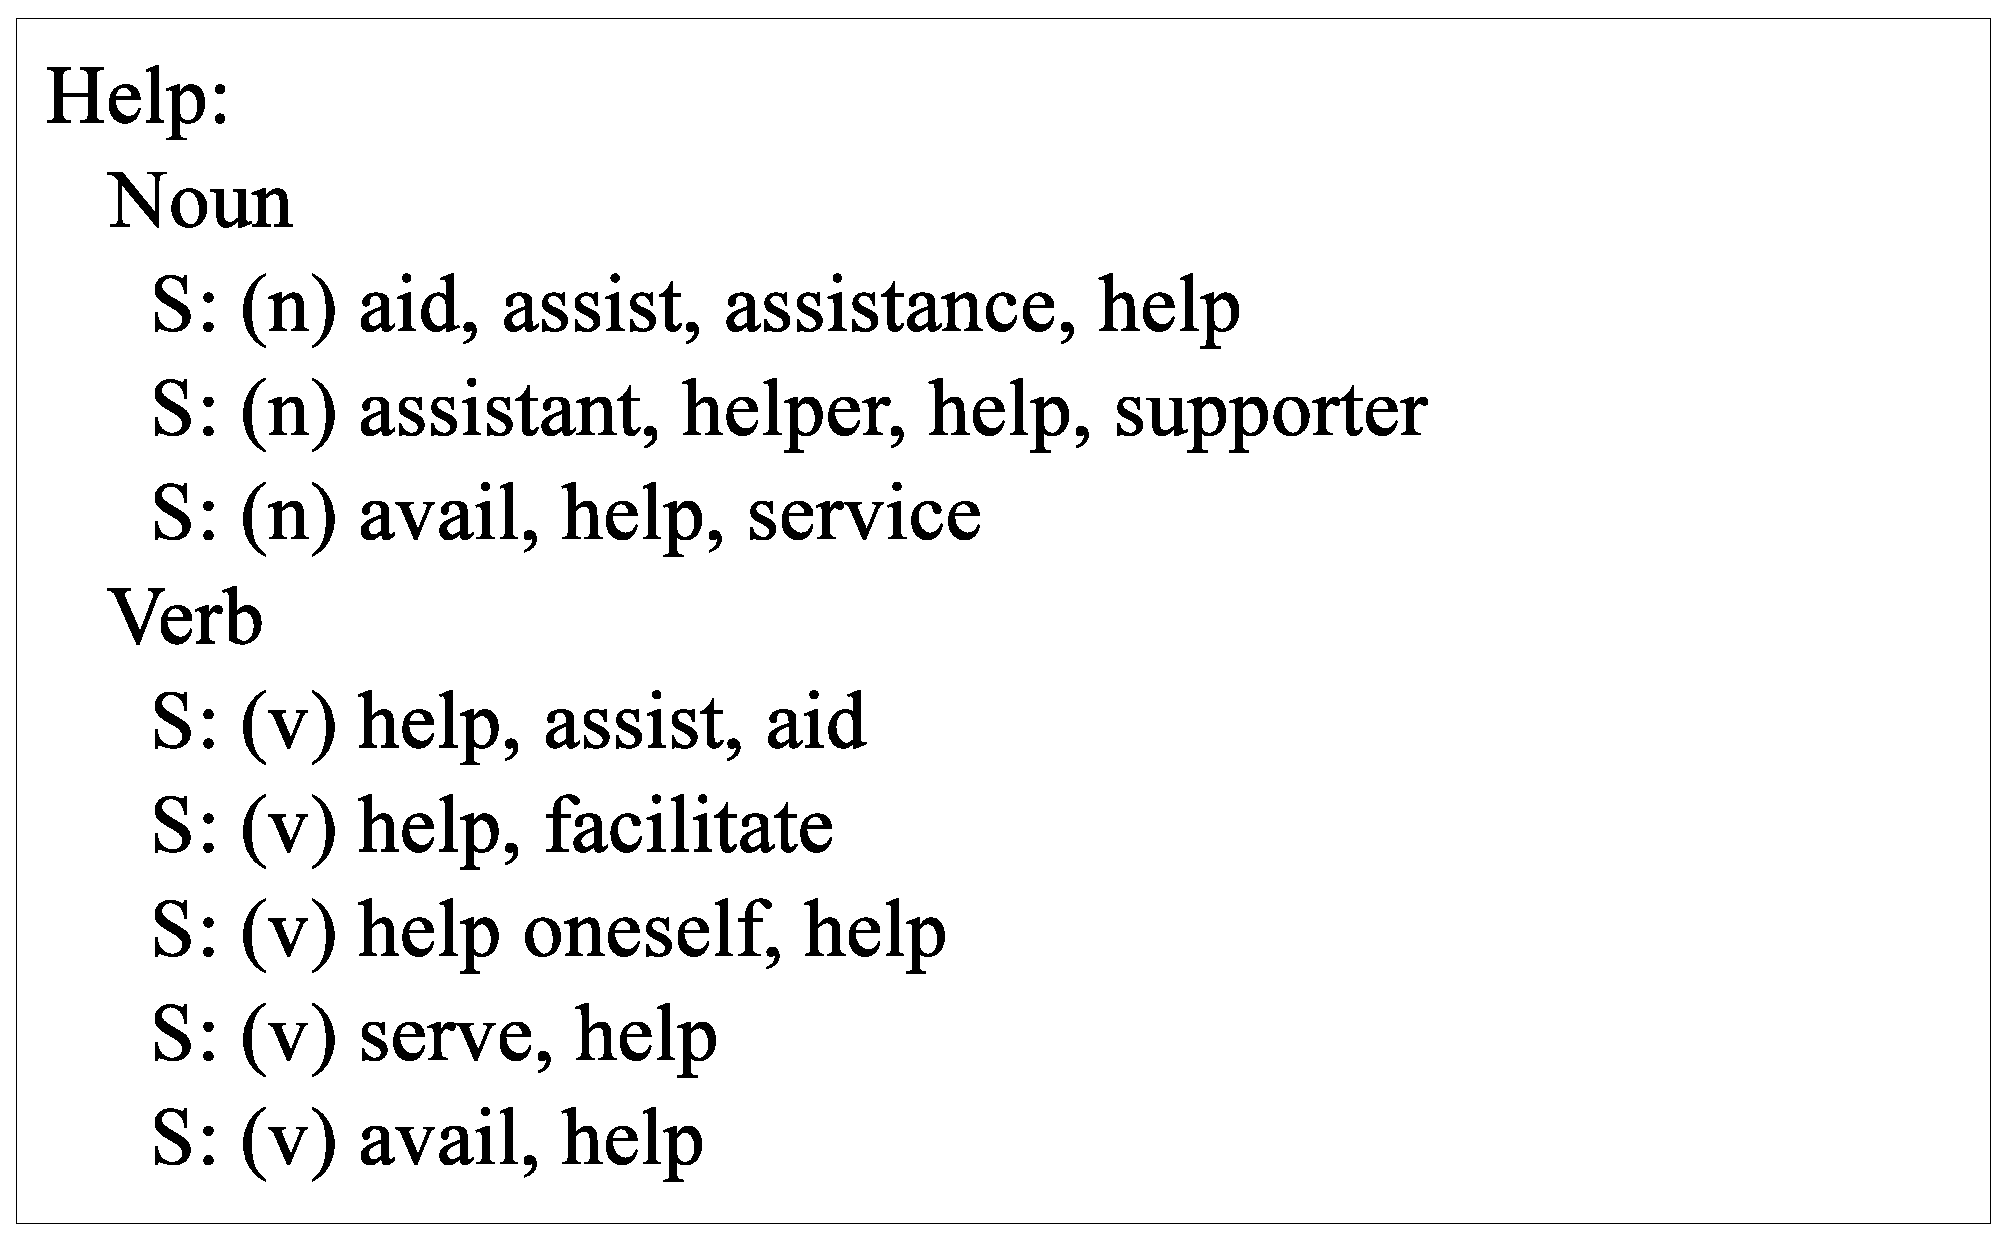
\includegraphics[height=180pt]{2-1-3.eps}
\caption{WordNet单词描述方式}
\label{fig2-2-3}
\end{figure}

\subsection{SentimentWordNet情感词典}
SentimentWordNet是Baccianella\upcite{Baccianella2010}等在语义词典WordNet基础上使用随机游走的图算法计算得到的情感词典。如图~\ref{fig2-2-4}所示,SentimentWordNet的每条记录都是一个WordNet的Synset条目,并且每个Synset都计算出了积极、消极情感极性的强度值(简称情感极性值),本章就是利用SentimentWordNet的情感极性值以及HowNet概念的语义关系进行计算得到中文词语的情感极性值,实现从英文情感词典到中文情感词典的情感知识转化。SentimentWordNet共有收录了117,000多个Synsets,约192,493单词。

\begin{figure}[htp]
\centering
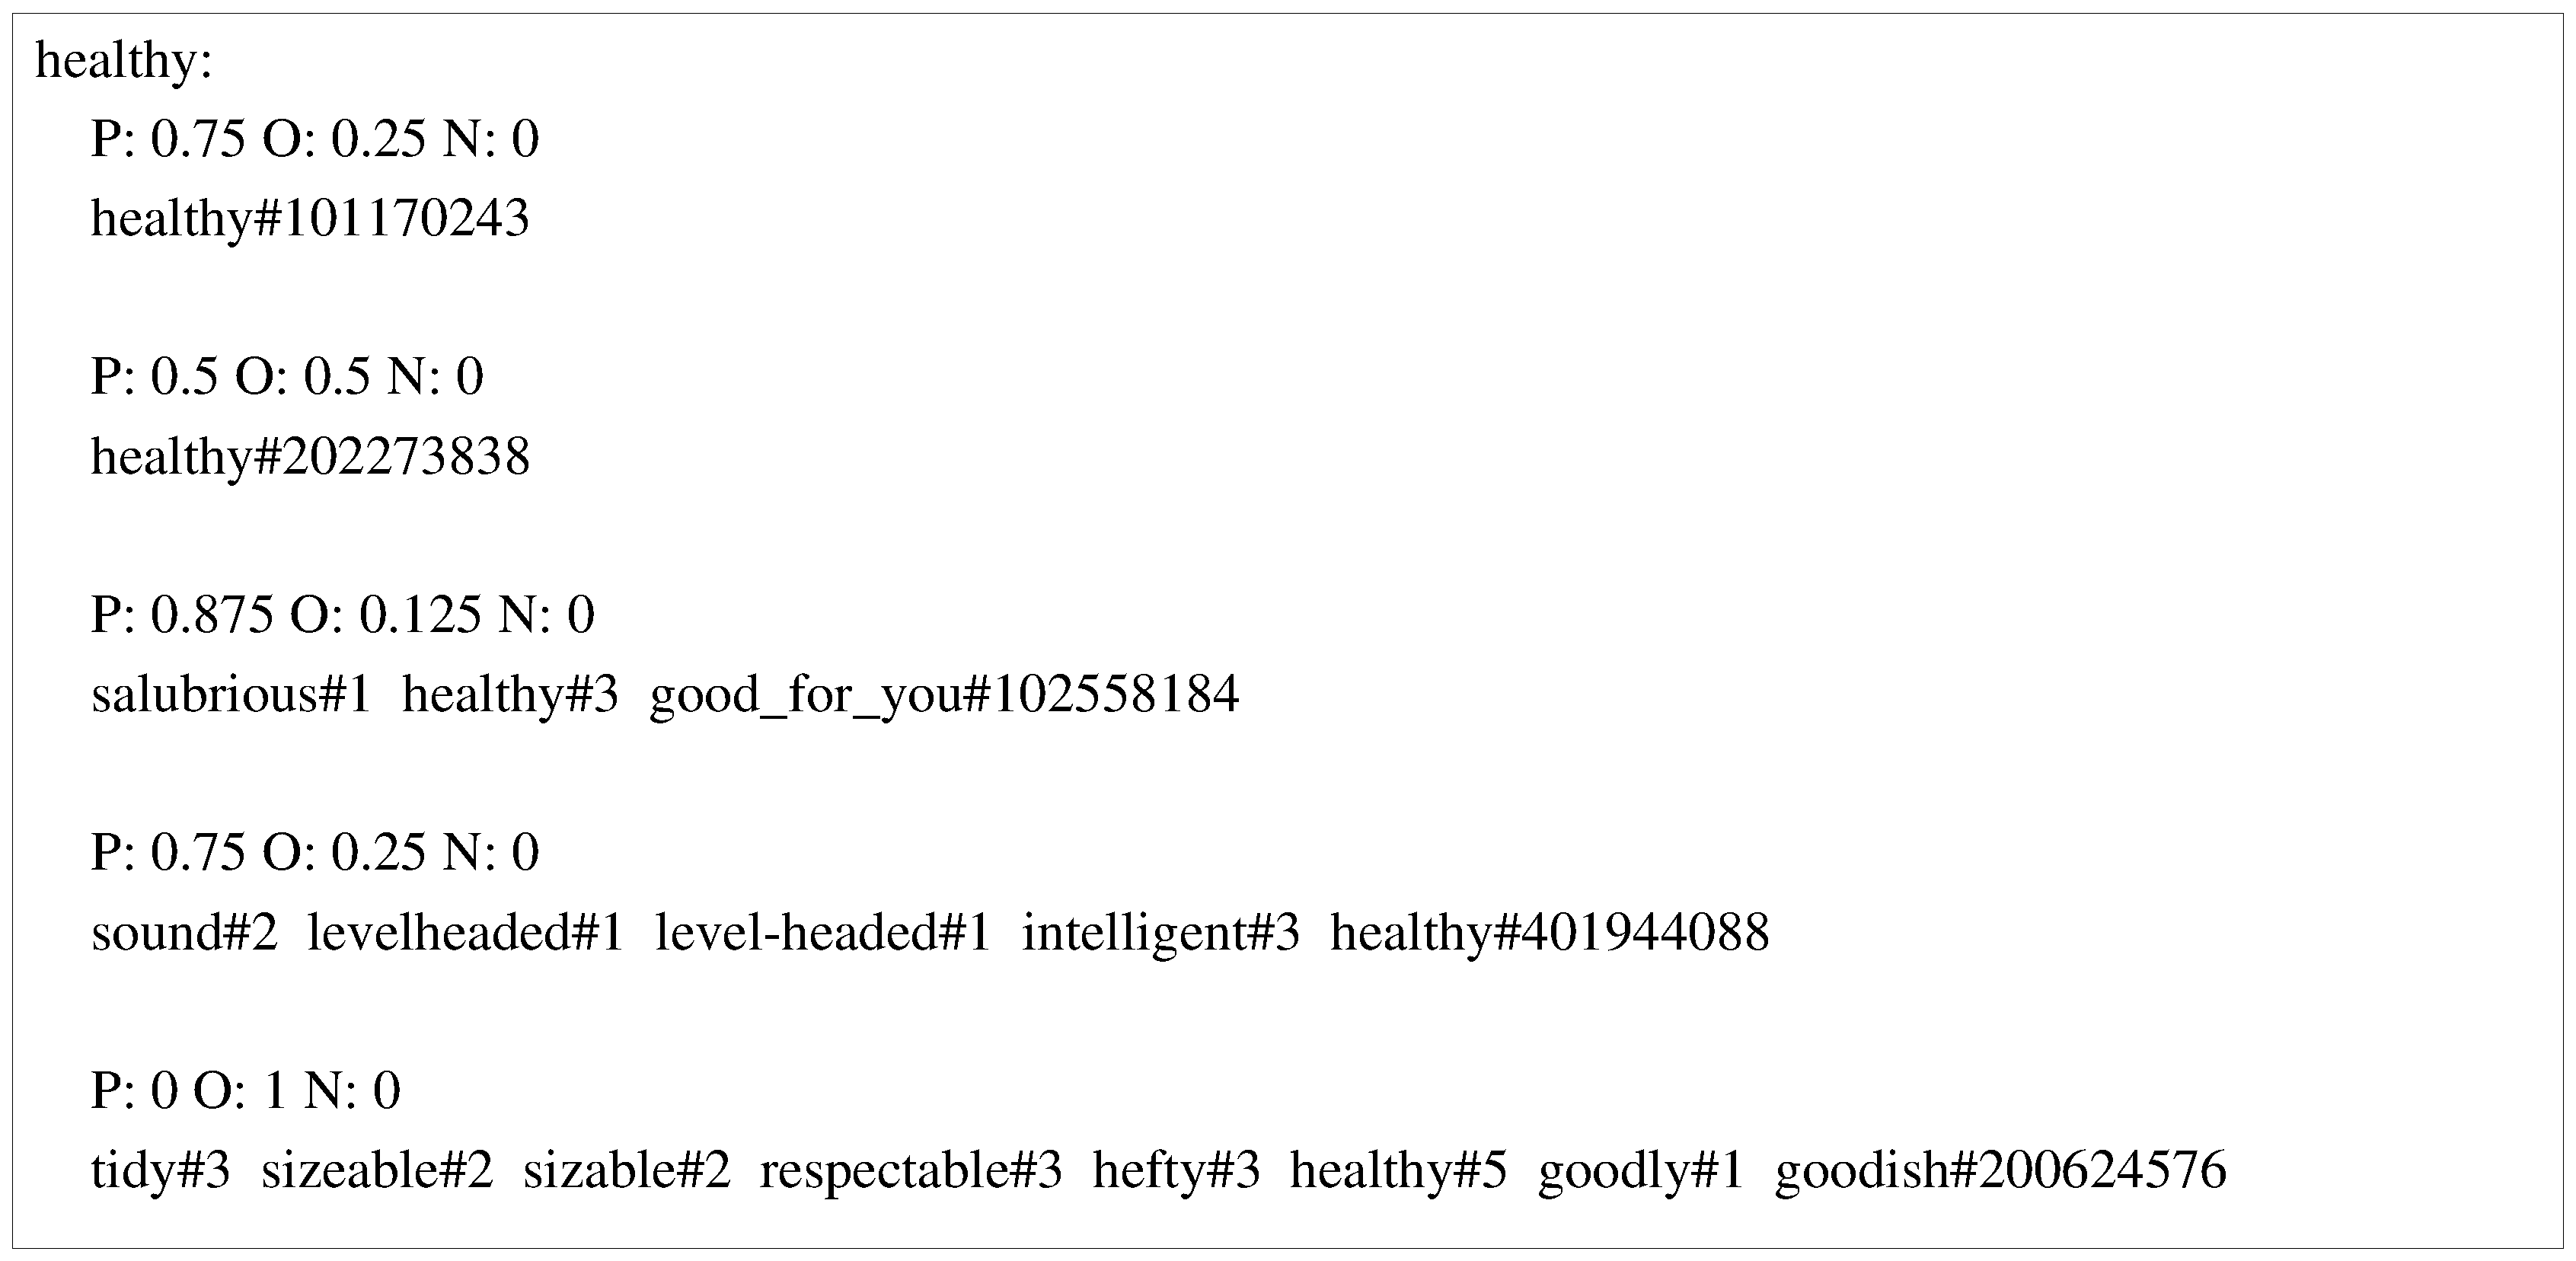
\includegraphics[height=220pt]{2-1-4.eps}
\caption{SentimentWordNet情感词描述方式}
\label{fig2-2-4}
\end{figure}

\section{基于语义关系的情感词典构建方法}
如本章相关工作部分所述,要构建一个新的情感词典有两种方式,一是从零开始(from scratch),另外一种就是通过转化(adaption)其他词典资源的方式。中文观点分析的研究在最近几年才开始受到重视,并且主要是借鉴英文研究已有的资源和方法。中文和英文语法结构和语义表示上存在很大的差别,直接套用英文的资源和研究方法会出现“水土不服”,比如直接将英文情感词典通过翻译方式转化的中文情感词典,是一个从英文情感知识到中文情感知识“给”的方式转化,是将英文情感词典内容映射到中文情感词典,因此存在歧义较大,覆盖度较低以及可靠性不高等问题,并且词典中不可避免存在翻译带来的错误。
本章提出一个从中文到英文情感词典去“取”的方式转化情感知识,是从中文情感词典到英文情感词典的逆映射,因此可以根据中文词语的语义单元选择英文对应语义单元然后转化情感知识,有效避免了歧义,而且不受覆盖度的限制,可靠性也更高。
同时可以直接将英文中对情感极性值的计算结果直接转化为中文词语的情感极性值,减少了计算开销。本章研究正是基于这种动机展开的,提出的解决方案如图~\ref{frame}框架所示。

具体来说,主要使用了双语语义知识库HowNet作为中文情感词语的来源以及对应英文查询词语的来源。HowNet对义原(都有英文标注)和概念(大部分都有英文标注)进行了英汉双语标注,可以作为中英文情感知识转化的“桥梁”。图~\ref{frame}计算框架中,每个词语的情感极性值的计算都是由三部分组成,首先是词语对应的英文标注可以从英文情感词典中查询获得情感极性值,第二部分是词语的语义描述DEF中会有义原的英文标注,也可以查询得到情感极性值,第三部分通过对语义描述DEF的语义关系分析,按照义原在DEF中的语义角色对其情感极性值加权后计算词语的情感极性值。

HowNet中有些词语本身没有英文标注,无法通过查询英文情感词典获得情感极性值。有些词语虽然有英文的标注,但是查询英文情感词典时候会遇到一词多义问题,不同语义对应的情感极性值不尽相同,得到的情感极性值也会因为存在歧义而不准确。还有一些词语标注的英文是多个单词,无法直接得到情感极性值。HowNet中词语的语义由概念表示,每个概念都有对应的语义描述DEF,DEF是由一个到多个义原按语义关系组合在一起的,因此概念在中文中是没有歧义的。本章正是利用了HowNet中概念语义描述部分,分析其中义原以及义原之间的关系,将义原情感极性值组合计算出词语的情感极性值。HowNet中义原是描述语义最基本的单位,可以假设义原的情感极性是确定的,基于此假设通过语义关系组合计算出的情感极性值也应该是确定的,因此可以对词语的情感极性进行“消歧”。

综上所述,本章构建情感词典需要解决的问题如下:
\begin{enumerate}
\item 如何基于英文情感词典计算义原的情感极性值?
\item 如何通过概念的语义描述中的语义关系分析组合计算概念的情感极性值?
\item 最后如何组合以上计算结果确定词语的情感极性值?
\end{enumerate}

针对这的三个问题,本章通过情感词语及义原抽取、义原情感极性值计算、以及词语情感极性值计算三个部分进行阐述。

\begin{landscape}
\begin{figure*}
\centering
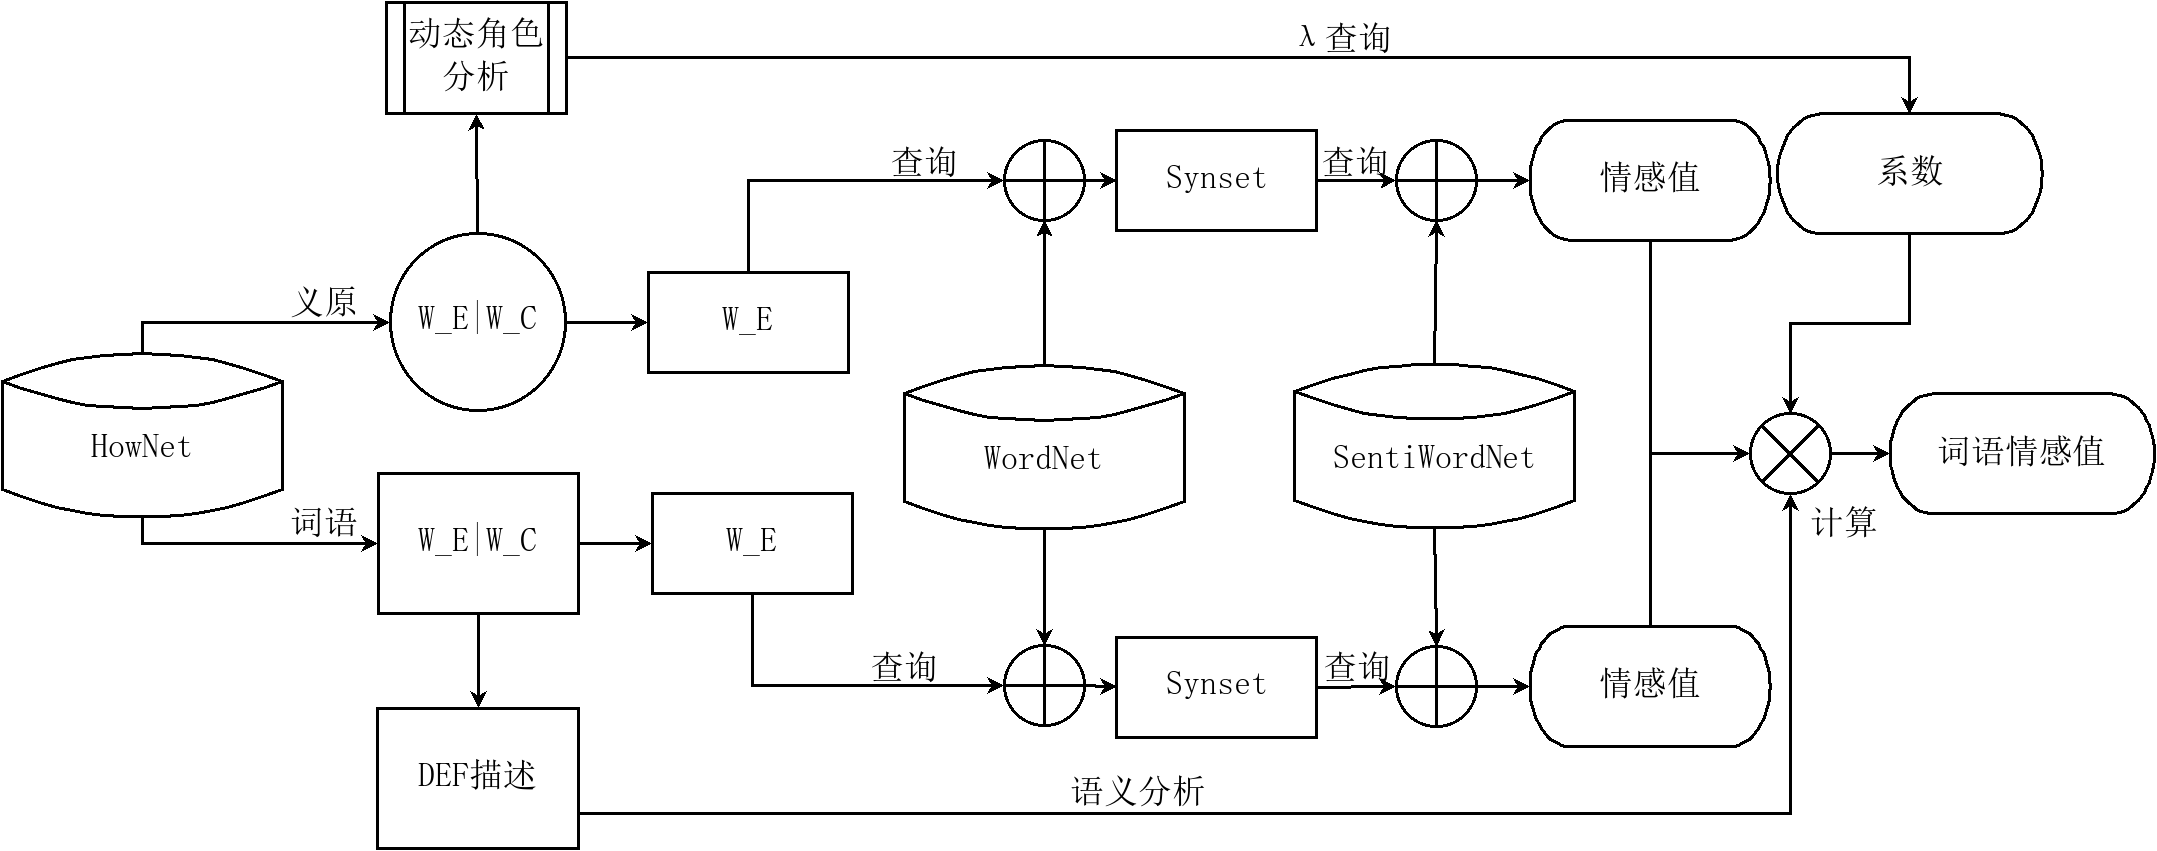
\includegraphics[height=250pt]{2-2.png}
\caption{基于语义关系情感词典构建方案}
\label{frame}
\end{figure*}
\end{landscape}

\subsection{词语和义原抽取}
词语抽取主要是从HowNet中抽取词语(W\_C)和概念描述(DEF),并对DEF进行分析得出其组成义原及语义关系描述符。在进行词语情感极性值计算时,需要根据DEF中义原和语义关系描述符进行词语的语义分析和极性值计算。情感词语和义原抽取处理流程如图~\ref{atom}所示。

\begin{figure}[htp]
\centering
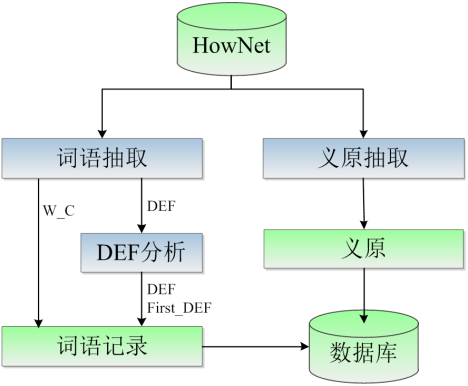
\includegraphics[height=170pt]{2-3.png}
\caption{词语和义原抽取处理流程}
\label{atom}
\end{figure}

从HowNet中抽取出的词语,定义其记录格式如图~\ref{fig2-2-1}所示。
在抽取得到的词语记录中,主要关注的内容有词语编号(No\.)、中文词语(W\_C)、中文词性(G\_C)、英文词语(W\_E)、英文词性(G\_E)、属性(DEF)、第一属性(First\_DEF)等。其中第一属性是指位于属性DEF第一位置的义原,通过第一属性可以分析出该词语所属的特征类。

\begin{figure}[htp]
\centering
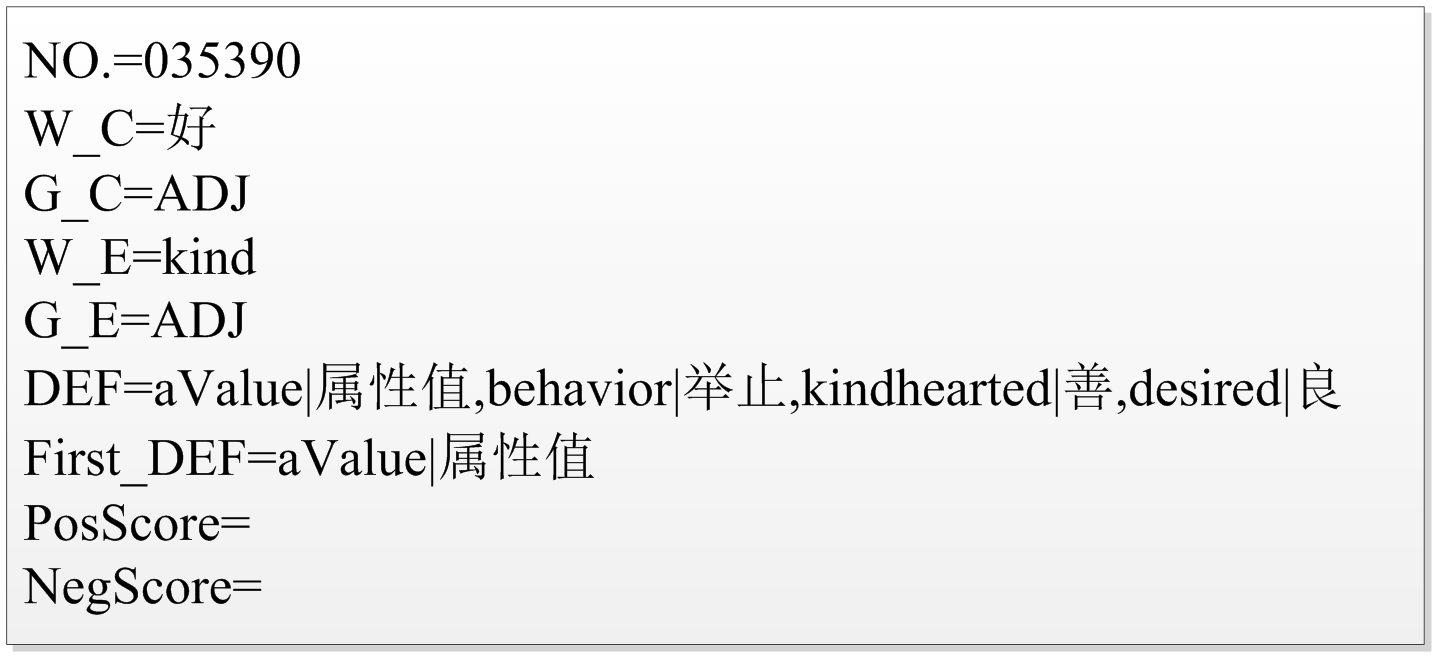
\includegraphics[height=125pt]{2-2-1.png}
\caption{抽取词语记录格式}
\label{fig2-2-1}
\end{figure}

从HowNet中抽取得到的义原的记录格式如图~\ref{fig2-2-2}所示。在抽取得到的义原的记录中,主要关注的内容有词语编号(No\.)、特征类别(Category)、中文词语(W\_C)、英文词语(W\_E)、属性(DEF)、层次(Layer)、父亲节点编号(Father)等。根据记录中的层次(Layer)和父亲节点编号(Father)可以得到义原之间的层次关系,如编号为33的义原“依靠”位于“事件类(Event)”的第五层,其父亲节点编号为32,通过查询编号为32的义原,得到其父亲节点义原为“有关(relate)”。

\begin{figure}[htp]
\centering
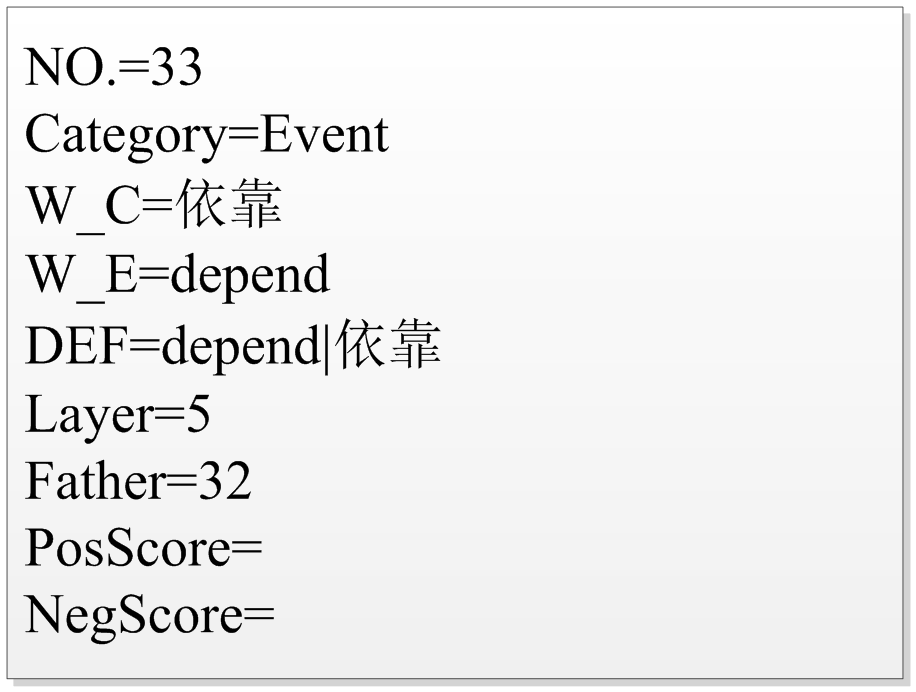
\includegraphics[height=125pt]{2-2-2.png}
\caption{抽取义原记录格式}
\label{fig2-2-2}
\end{figure}

\subsection{义原情感极性值}
在词语情感极性值计算中,义原的情感极性值的确定是非常关键的,是计算词语情感极性值的基础。在HowNet中义原都使用中英双语标注,基本都可以根据英文标注查询得到情感极性值(称为查询类义原极性值)。也有一部分义原英文标注由多个单词连接组成(如“FreeOfCharge$ | $免费”),无法直接查询得到情感极性值,可以通过在上下位关系树中与其他义原的语义距离进行计算获得(称为计算类义原极性值)。最后可以通过义原间的反义和对义关系对计算出的义原情感极性值进行校正。

\subsubsection{查询类义原极性值}
WordNet是以词义(Sense)来记录的,Sense以同一词义的词集Synset表示。通过查询可以得到词语W\_E所有的Sense,将每个Sense映射到SentimentWordNet就可以得到对应的情感极性值。
基于WordNet和SentimentWordNet的义原极性值计算过程如图~\ref{atomsen}所示。

\begin{figure}[htp]
\centering
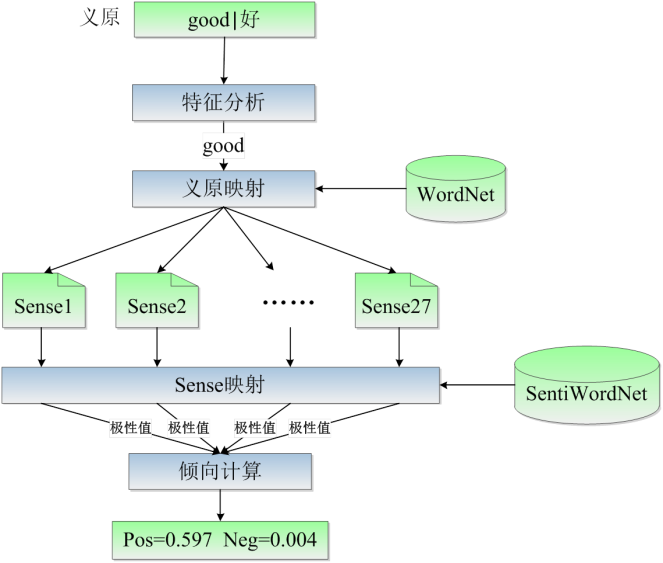
\includegraphics[height=250pt]{2-4.png}
\caption{义原情感极性值计算过程}
\label{atomsen}
\end{figure}

在HowNet中获取义原后将义原对应英文单词(如“good”)映射到WordNet中进行查询,得到该词语所有的Sense(如“good”的Sense共有27个);将这些Sense再映射到SentimentWordNet中查询得到对应Sense情感极性值;将情感极性值加权根据公式~\ref{eq1}计算得到义原的情感极性值(如“good”的极性值为PosScore=0.597,NegScore=0.004)。
\begin{equation}
\label{eq1}
\varphi(s,p)=\dfrac{\sum_{i=1} \varphi_i (s,p)}{\sum_{p\in P}\sum_{i=1}^m \varphi_i(s,p)}
\end{equation}

公式中$ P$表示极性类型(积极(P)和消极(N)),$m$为与义原相对应的Sense的总数,$s$表示义原,$\varphi(s,p)$表示义原的极性值,$\varphi_i (s,p)$表示义原在编号为$ i $的Sense中的$ p $类型极性值。

\subsubsection{计算类义原极性值}
经过上面的查询计算过程,可以得到大部分义原的情感极性值。由于所有的义原根据上下位关系构成了一个树状的义原层次体系,针对一些无法通过查询计算得到情感极性值的义原,可以使用语义距离计算相似度的办法间接计算出情感极性值。假设两个义原(一个情感极性值已知,一个未知)在上下位层次体系中的路径距离为$ d $,根据公式~\ref{eq2-1},可以得到这两个义原之间的语义距离:
\begin{equation}
\label{eq2-1}
sim(s_i,s)=\dfrac{\alpha}{d+\alpha}
\end{equation}
其中$ s_i $是情感极性值已知义原,$ s $表示需要情感极性值计算的义原,$ d $是$ s_i $和$ s $在义原层次体系树中的路径长度。$ \alpha $是一个可调节的参数,一般$ \alpha=0.5 $。

为了能够在上位和下位义原的情感极性值取得平衡,对任意一个情感极性值未知义原$ s $,都要计算$ s $与最靠近$ s $极性值已知的上位义原$ s_1 $ 和下位义原 $ s_2 $之间的语义距离:$sim(s_1,s)$和$sim(s_2,s)$。然后对上位义原$ s_1 $ 和下位义原 $ s_2 $的情感极性值加权平均得到$ s $的情感极性值。
\begin{equation}
\varphi(s,p)=sim(s_1,s)\varphi(s_1,p)+sim(s_2,s)\varphi(s_2,p)
\end{equation}

\subsubsection{情感极性值校正}
所有义原使用前面两种方法计算得到情感极性值会存在一些偏差(bias),有些义原偏差会比较大,甚至计算得到的极性值与义原的真实语义倾向相反(如“FreeOfCharge$ | $免费”义原计算得到极性值为PosScore=0.07,NegScore=0.236),因此需要通过利用HowNet中的其他语义关系对上述计算方法进行校正。在此采用了基于HowNet中对义和反义语义关系进行义原情感极性值校正。对于任一义原$ s $,对义或反义义原为$ \overline{s} $,对$ s $情感极性值修正为:
\begin{equation}
\varphi(s,p)=\dfrac{|\varphi(s,p)-\varphi(\overline{s} ,p)|}{2}
\end{equation}



\subsection{词语情感极性值}
词语情感值可以通过两种途径获得,一是通过词语本身的英文标注直接查询英文情感词典,这种方式并不可靠而且存有歧义;二是根据词语的语义描述DEF中的义原的情感极性值计算得出,这种方式相对可靠,每个义原都有确定的情感极性值,因而不存在歧义。为了计算词语的情感极性值,需要对语义描述DEF中的语义关系进行分析,因为义原间的语义关系会引起义原情感值的反转或者在描述语义倾向时的权重变化。
首先对HowNet中因为DEF的语义关系不同引起的情感极性值变化提出如下定义:
\begin{definition}[情感极性值反转]
义原$s$的$p$极性值$\varphi(s,p)$取反运算是,将$s$的积极极性值和消极极性值互换,过程如公式~\ref{2-2}:
\begin{equation}
\label{2-2}
\overline{\varphi(s,p)}=\varphi(s,q),\quad p,q \in P\&\& p \neq q
\end{equation}
\end{definition}
事件类义原有很多在DEF描述中可以引起情感极性值的变化,比如“DoNot$ | $不做,lose$ | $失去”等相当于句子中的否定词,会引起其他词语情感极性值反转,因此本章从819个事件类义原中挑选了在语义描述中起否定作用的义原称为极性反转语义角色,并加以标记。
\begin{definition}[情感极性值加权]
 $\lambda$因子与义原$s$的$p$极性值的加权运算定义为$\lambda$乘法运算,过程如公式~\ref{2-3}:
\begin{equation}
\label{2-3}
\lambda \times \varphi(s,p) =\begin{cases}
& \lambda \varphi(s,p), \quad  \lambda >0\\
& 0, \quad\quad  \lambda=0\\
&|\lambda|\varphi(s,p), \quad  \lambda <0
\end{cases}
\end{equation}
\end{definition}

公式~\ref{2-3}中$\lambda$取值范围为$ \{-1,0,1\} $,具体值需要根据关系义原描述式中的关系义原(动态角色义原)和符号义原描述式中的符号义原确定。符号义原中只有“$ \wedge$”(表示“非”的关系)会改变语义倾向,因此“$ \wedge$”所修饰的义原在计算中权重为$\lambda=-1$。
HowNet中共有90个动态角色义原,本章分别对每个义原进行了分析,确认了其语义关系角色所确定的基本义原的权重取值$\lambda$。
如词语“扭亏为盈”的DEF描述为“DEF=alter|改变,StateIni=InDebt|亏损,StateFin=earn|赚”,义原“InDebte|亏损”为初始状态(StateIni),“earn|赚”为最终状态(StateFin),经过分析后,StateIni描述的“InDebte|亏损”的$\lambda$取值为0,StateFin描述的“earn|赚”的$\lambda$取值为1。

词语的情感极性值计算总结为公式~\ref{2-4}。其中$\varphi(w,p)$表示词语$w$的$p$极性值,$s_i$表示词语DEF中第$i$个义原,$n$为词语DEF中义原总数。
\begin{equation}
\label{2-4}
\varphi(w,p)=\dfrac{\sum_{i=1}^n\lambda_i\times\varphi(s_i,p)}{\sum_{p\in P}\sum_{i=1}^n\lambda_i\times\varphi(s_i,p)}
\end{equation}
其中:$\sum_{p \in P}\varphi(w,p)=1$。

对于已经通过查询得到情感极性值的词语(有多个英文Sense对应的词语的情感极性值$\varphi(\overline{w},p)$,取所有Sense对应极性值的加和平均),可以和通过语义描述DEF计算得到的极性值加权累加,计算公式为:
\begin{equation}
\Psi(w,p)=\alpha \varphi(w,p)+(1-\alpha)\varphi(\overline{w},p)
\end{equation}
其中$ \alpha \in (0,1)$的取值要考虑那种方式得到的情感极性值更准确,一般将$ \alpha $取大些以反映语义描述DEF对词语语义倾向性的影响更大。

\section{实验}
情感词典的实验评测有两种方法,一是直接评测,将情感词典与人工编辑的或者其他可靠性较高的词典进行对比评测;二是间接评测,将情感词典应用到文本情感分类任务评测其性能。本节使用直接评测的方法。

\subsection{直接评测}
在实验评测时,采用HowNet评价词词典基准。HowNet评价词词典是2007年发布的人工标注的词典,每个词语只标注积极和消极极性,没有准确的情感极性值信息。HowNet评价词词典中情感词共有6497项,其中积极极性词语3436项,消极极性词语3061项。

在此将本章中利用HowNet中的语义关系构建的情感词典命名为SentiHowNet。SentiHowNet的词语都有积极极性值和消极极性值,为了和HowNet评价词词典作对比评测,按照公式~\ref{eq2-5}对SentiHowNet的每个词计算得出一个极性。
\begin{equation}
\label{eq2-5}
Polarity(w)=\begin{cases}
positive \qquad & score(w)>T\\
negative \qquad & score(w)<-T
\end{cases}
\end{equation}
其中$ score(w)= \varphi(w,P)-\varphi(w,N)$为词语$ w $积极极性值与消极极性值相减得到的差值,$ T $为阈值,差值$ score(w)$高于$ T $则词语$ w $情感极性为积极极性,差值$ score(w)$低于$ -T $则词语$ w $情感极性为消极极性。当$ T=0 $时,我们构建的SentiHowNet有积极极性情感词12433项,消极极性情感词11148,词典的整体规模达到23581个条目。

评价指标采用常用宏平均和微平均的精准率(P)、召回率(R)以及F值。
\subsubsection{阈值T的设定}
首先考察不同的阈值$ T $对词典评价指标的影响,以确定一个合理的阈值。
图\ref{fig2-5}为$ T $的不同取值对词典性能指标的影响,实验中将$ T $的值由0逐渐增加,当$ T $大于0.1时性能指标基本没有变化或成下降趋势。从图中可以看出,在$ T=0 $时,虽然召回率最高达到88.58\%,但精准率最低仅有54.40\%,F值仅为67.40\%。当$ T=0.05 $时,精准率提高到77.75\%,有较大提高,召回率仅下降到87.61\%,下降幅度较小,F值提高到82.39\%。当$ T $提高到0.05时性能指标达到最好,因此可以设定$ T $为0.05。

\begin{figure}[htp]
\centering
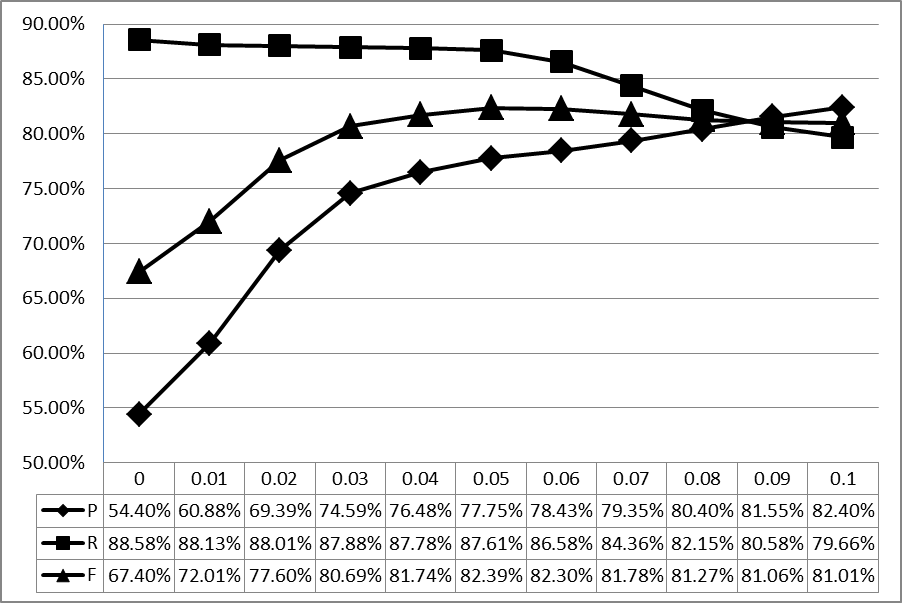
\includegraphics[height=220pt]{2-5.png}
\caption{不同T值时的性能指标}
\label{fig2-5}
\end{figure}

\subsubsection{与其他词典性能对比}
确定了阈值T以后,实验中将SentiHowNet与目前常用的中文情感词典NTUSD词典(11086个中文词汇,2810积极极性词语,8276消极性词语)\upcite{Ku2007}以及大连理工大学的情感词汇本体词库(用DLLEX标记,17156条目,10627个积极极性词语,6529个消极极性词语)\upcite{徐琳宏2008}进行对比评测。首先是三个词典对评价基准词典的覆盖度对比,结果如表~\ref{tab2-2}所示。从表中可以看出,如果按照积极和消极极性分开来看,在积极极性词中SentiHowNet词典覆盖度最好,NTUSD词典由于包含的积极极性词数量少因此覆盖读最低;在消极极性词中,NTUSD词典的覆盖度最好,SentiHownet和DLLEX词典覆盖度基本一样。四种个词典中除了作为基准词典的HowNet评价词词典,采用本章设计方法在HowNet上自动构建的情感词典SentiHowNet包含情感词条目(注意经过阈值T=0.05过滤后)最少,但是对基准词典的覆盖度最高(总体准确标注数达到6092),主要原因是SentiHowNet本身就是从HowNet自动产生,是HowNet包含词语的子集,而NTUSD和DLLEX词典中词语的来源不同,因此会有覆盖度的偏置。

\begin{table}[htp]
\centering
\caption{词典覆盖度}
\label{tab2-2}
\begin{tabular}{|l|l|l|l|l|l|l|}
\hline
\multicolumn{1}{|c|}{\multirow{2}{*}{词典}} & \multicolumn{2}{c|}{积极极性} & \multicolumn{2}{c|}{消极极性} & \multicolumn{2}{c|}{总体统计} \\ \cline{2-7} 
\multicolumn{1}{|c|}{} & \multicolumn{1}{c|}{标注} & \multicolumn{1}{c|}{正确} & \multicolumn{1}{c|}{标注} & \multicolumn{1}{c|}{正确} & \multicolumn{1}{c|}{标注} & \multicolumn{1}{c|}{准确} \\ \hline
HowNet & \multicolumn{2}{c|}{3436} & \multicolumn{2}{c|}{3061} & \multicolumn{2}{c|}{6497} \\ \hline
NTUSD & 2810 & 2204 & 8276 & 3022 & 11086 & 5226 \\ \hline
DLLEX & 10627 & 3020 & 6529 & 2876 & 17156 & 5896 \\ \hline
SentiHownet & 4256 & 3218 & 5113 & 2874 & 9369 & 6092 \\ \hline
\end{tabular}
\end{table}

在T=0.05时,SentiHowNet与其他词典性能比较如表~\ref{tab2-3}所示。在积极极性词语的性能对比中,SentiHowNet词典的精确率和F值最好,分别达到了93.66\%和83.67\%,但是召回率(75.\%61)比NTUSD词典(78.43\%)略差;在消极极性词语的性能对比中,三个词典的精确率都比较高(都超过90\%),但是召回率比较低,NTUSD词典精确率最好,达到98.73\%,而SentiHowNet词典在召回率和F值上性能最好;总体来看,宏平均指标中SentiHowNet词典精准率为93.77\%,召回率为65.02\%,F值为76.79\%,均为三个词典中最高。
\begin{table}[htp]
\centering
\caption{词典性能对比}
\label{tab2-3}
\begin{tabular}{|l|c|c|c|c|c|c|c|c|c|}
\hline
\multicolumn{1}{|c|}{\multirow{2}{*}{词典}} & \multicolumn{3}{c|}{积极极性} & \multicolumn{3}{c|}{消极极性} & \multicolumn{3}{c|}{宏平均} \\ \cline{2-10} 
\multicolumn{1}{|c|}{} & P & R & F & P & R & F & P & R & F \\ \hline
NTUSD & 0.6414 & \textbf{0.7843} & 0.7057 & \textbf{0.9873} & 0.3652 & 0.5331 & 0.8044 & 0.4714 & 0.5944 \\ \hline
DLLEX & 0.8789 & 0.2842 & 0.4295 & 0.9396 & 0.4405 & 0.5998 & 0.9075 & 0.3437 & 0.4985 \\ \hline
SentiHownet & \textbf{0.9366} & 0.7561 & \textbf{0.8367} & 0.9389 & \textbf{0.5621} & \textbf{0.7032} & \textbf{0.9377} & \textbf{0.6502} & \textbf{0.7679} \\ \hline
\end{tabular}
\end{table}

以上两个对比表明相对于需要人工干预的人工或半自动方法构建的情感词典,使用本章设计的自动构建情感词典方法可以构建一部覆盖度比较好,性能又可靠的情感词典,同时节省了不必要的人力开销。

\section{小结}
本章对中文情感词典构建相关研究进行了分类和详细阐述,基于目前中文情感词典研究现状,提出了一种新的跨语言情感词典自动转化方法。该方法以双语语义知识库HowNet、WordNet语义词典和SentimentWordNet情感词典为基础,根据HowNet对词语语义定义和描述的特点,通过双语标注将HowNet义原和词语情感值转换为英文情感词典对应词语的查询与计算。具体来说,中文词语的情感极性值计算被分解为三个部分,分别为义原情感值的计算与校正,词语语义描述的语义关系分析以及最终的词语情感值的计算。按照该方法最终形成情感词典SentiHowNet,词典的规模为:积极极性情感词12433项,消极极性情感词11148项,词典的整体规模达到23581个条目。在实验部分,采用了直接评测的方法,以人工编辑的HowNet评价词典为基准,在覆盖度、精确率、召回率以及F值等指标上与现有的常用情感词典NTUSD和DLLEX词典进行了实验对比。实验结果表明,SentiHowNet对基准词典的覆盖度最好,宏平均的精确率、召回率以及F值最高,证明了该自动构建情感词典方法的有效性,避免了人工和半自动方法的人工干预开销。
\newpage 
\mbox{} 
\newpage


%%% Local Variables:
%%% mode: latex
%%% TeX-master: "../main"
%%% End:

\begin{ack}
“Learning is more imortant than knowing”,尤其是对于工作过一段时间的人来说,在感知到自己所知甚少时候能有机会重新学习,进行课题研究,需要感谢的人实在是太多。

首先感谢我的导师王挺教授,从一开始能够接受一名在职的考博学生,您就以开放而又严谨的治学态度给予我最大的支持,感谢您在过去的五年中精细的学术指导和研究建议,您在学术领域的专业深度和开阔视野激发了我在文本信息处理研究的巨大兴趣,感谢您让我拥有充分的研究自由,培养了我深入思考和独立解决问题的能力,这些都对于我顺利完成博士课题研究都是必不可少的。

感谢课题组的唐晋韬、周云、李岩、麻大顺、刘培磊、岳大鹏、刘海池、汝承森、张文文、姜仁会、胡长龙、李欣奕,和大家一起亦师亦友共同探讨自然语言处理领域最前沿的问题让我获益非浅,在艰辛的求学到路上大家互相帮助,苦中作乐的日子让我重新体会到了无私的同学友谊。

感谢计算机学院的学院领导在工作、考博和学习期间给我的关怀和指导;感谢学员大队的同事,在我求学阶段给我指导、鼓励还有协助;感谢博士队队领导和各位博士战友,在一起“共同战斗”的日子永远值得回味。

最后,也是做重要的,感谢我的家人,没有家人的支持就没有我顺利的博士学习研究:感谢我的妻子黄丽达,感谢你牺牲自己的工作学习对我的支持;感谢我五岁的女儿,你的出生给我生活带来无尽的乐趣;感谢我的岳父母,在我读博期间对我们这个小家的生活上无微不至的照顾;感谢在山东的父母,远在千里你们的关爱依然!
\end{ack}
\newpage 
\mbox{} 
\newpage

%</thesis>
%    \end{macrocode}
%
% 在\LaTeX{}下管理参考文献将极其方便,建议使用Jabref生成条目,
% 用\verb|\cite|(其中\verb|upcite|是上标索引)索引即可。
% \verb|refs.bib|是你的参考文献名。
%    \begin{macrocode}
%<*thesis>
\cleardoublepage
\phantomsection
\addcontentsline{toc}{chapter}{参考文献}
\bibliographystyle{bstutf8}
\bibliography{ref/refs}

\begin{resume}

  \section*{发表的学术论文} % 发表的和录用的合在一起

  \begin{enumerate}[{[}1{]}]
  \addtolength{\itemsep}{-.36\baselineskip}%缩小条目之间的间距,下面类似
  
  \item Zhunchen Luo, Miles Osborne, Sasa Petrovic and Ting Wang. Improving Twitter Retrieval by Exploiting Structural Information. In {\it Proceedings of the Twenty-Sixth AAAI Conference on Artificial Intelligence} (\textbf{AAAI 2012}), Toronto, Canada, July 2012. \textbf{(CCF A类会议,人工智能领域顶级会议)}
 
 \item Zhunchen Luo, Miles Osborne, Jintao Tang and Ting Wang. Who Will Retweet Me? Finding Retweeters in Twitter. In {\it Proceedings of the Thirty-Sixth International ACM SIGIR Conference on Research and Development in Information Retrieval} (\textbf{SIGIR 2013}), Dublin, Ireland, July 2013.\textbf{(CCF A类会议,信息检索领域顶级会议,获得会议旅行奖金1300美元)}

\item Zhunchen Luo, Miles Osborne and Ting Wang. Opinion Retrieval in Twitter. In {\it Proceedings of the Sixth International AAAI Conference on Weblogs and Social Media} (\textbf{AAAI-ICWSM 2012}), Dublin, Ireland, June 2012. \textbf{(社交媒体领域顶级会议,获得会议旅行奖金300美元)}

 \item  Zhunchen Luo, Miles Osborne and Ting Wang. An Effective Approach to Tweets Opinion Retrieval. To appear in \textbf{World Wide Web Journal}. (\textbf{SCI期刊,影响因子1.196})
 
 \item Zhunchen Luo, Jintao Tang and Ting Wang. Propagated Opinion Retrieval in Twitter. In {\it Proceedings of the Fourteenth International Conference on Web Information System Engineering} (\textbf{WISE 2013}), Nanjing, China, October 2013.\textbf{(CCF C类会议,信息检索与数据挖掘领域重要会议)}

\item Zhunchen Luo, Jintao Tang and Ting Wang. Improving Keyphrase Extraction from Web News by Exploiting Comments Information. In {\it Proceedings of the Fifteenth International Asia-Pacific Web Conference} (\textbf{APWeb 2013}), Sydney, Australia, April 2013. \textbf{(CCF C类会议,信息检索与数据挖掘领域重要会议)}

\item Zhunchen Luo, Lan Rao, Chengsen Ru and Ting Wang. Finding High-Quality Posts from Microblogging Conversations. In {\it the Eighth International Conference on Modeling Decisions for Artificial Intelligence (\textbf{MDAI 2011})}, Changsha, China, July, 2011.

\item 罗准辰,王挺. 基于分离模型的中文关键词提取算法研究. 中文信息学报, 2009,23 (01): 63-70.

\item 罗准辰,王挺. 搜索词同现网络研究. 第六届全国信息检索学术会议(\textbf{CCIR 2010}),镜泊湖,2010年8月.

  \end{enumerate}

\end{resume}

%</thesis>
%    \end{macrocode}
%
%<thesis>% 最后,需要的话还要生成附录,全文随之结束。
%    \begin{macrocode}
%<*thesis>
\appendix
\backmatter
% TeX
\chapter{模板提供的希腊字母命令列表}

大写希腊字母:
\begin{table}[htbp]
\centering
\begin{tabular}{llll}
\toprule
$\Gamma$~\verb|\Gamma| & $\Lambda$~\verb|\Lambda| & $\Sigma$~\verb|\Sigma| & $\Psi$~\verb|\Psi| \\
$\Delta$~\verb|\Delta| & $\Xi$~\verb|\Xi| & $\Upsilon$~\verb|\Upsilon| & $\Omega$~\verb|\Omega| \\
$\Theta$~\verb|\Theta| & $\Pi$~\verb|\Pi| & $\Phi$~\verb|\Phi| & \\
\midrule
$\varGamma$~\verb|\varGamma| & $\varLambda$~\verb|\varLambda| & $\varSigma$~\verb|\varSigma| & $\varPsi$~\verb|\varPsi| \\
$\varDelta$~\verb|\varDelta| & $\varXi$~\verb|\varXi| & $\varUpsilon$~\verb|\varUpsilon| & $\varOmega$~\verb|\varOmega| \\
$\varTheta$~\verb|\varTheta| & $\varPi$~\verb|\varPi| & $\varPhi$~\verb|\varPhi| & \\
\bottomrule
\end{tabular}
\end{table}

小写希腊字母:
\begin{table}[htbp]
\centering
\begin{tabular}{llll}
\toprule
$\alpha$~\verb|\alpha| & $\theta$~\verb|\theta| & $o$~\verb|o| & $\tau$~\verb|\tau| \\ 
$\beta$~\verb|\beta| & $\vartheta$~\verb|\vartheta| & $\pi$~\verb|\pi| & $\upsilon$~\verb|\upsilon| \\ 
$\gamma$~\verb|\gamma| & $\iota$~\verb|\iota| & $\varpi$~\verb|\varpi| & $\phi$~\verb|\phi| \\ 
$\delta$~\verb|\delta| & $\kappa$~\verb|\kappa| & $\rho$~\verb|\rho| & $\varphi$~\verb|\varphi| \\ 
$\epsilon$~\verb|\epsilon| & $\lambda$~\verb|\lambda| & $\varrho$~\verb|\varrho| & $\chi$~\verb|\chi| \\ 
$\varepsilon$~\verb|\varepsilon| & $\mu$~\verb|\mu| & $\sigma$~\verb|\sigma| & $\psi$~\verb|\psi| \\ 
$\zeta$~\verb|\zeta| & $\nu$~\verb|\nu| & $\varsigma$~\verb|\varsigma| & $\omega$~\verb|\omega| \\ 
$\eta$~\verb|\eta| & $\xi$~\verb|\xi| & $\varkappa$~\verb|\varkappa| & $\digamma$~\verb|\digamma| \\ 
\midrule
$\upalpha$~\verb|\upalpha| & $\uptheta$~\verb|\uptheta| & $\mathrm{o}$~\verb|\mathrm{o}| & $\uptau$~\verb|\uptau| \\ 
$\upbeta$~\verb|\upbeta| & $\upvartheta$~\verb|\upvartheta| & $\uppi$~\verb|\uppi| & $\upupsilon$~\verb|\upupsilon| \\ 
$\upgamma$~\verb|\upgamma| & $\upiota$~\verb|\upiota| & $\upvarpi$~\verb|\upvarpi| & $\upphi$~\verb|\upphi| \\ 
$\updelta$~\verb|\updelta| & $\upkappa$~\verb|\upkappa| & $\uprho$~\verb|\uprho| & $\upvarphi$~\verb|\upvarphi| \\ 
$\upepsilon$~\verb|\upepsilon| & $\uplambda$~\verb|\uplambda| & $\upvarrho$~\verb|\upvarrho| & $\upchi$~\verb|\upchi| \\ 
$\upvarepsilon$~\verb|\upvarepsilon| & $\upmu$~\verb|\upmu| & $\upsigma$~\verb|\upsigma| & $\uppsi$~\verb|\uppsi| \\ 
$\upzeta$~\verb|\upzeta| & $\upnu$~\verb|\upnu| & $\upvarsigma$~\verb|\upvarsigma| & $\upomega$~\verb|\upomega| \\ 
$\upeta$~\verb|\upeta| & $\upxi$~\verb|\upxi| & & \\ 
\bottomrule
\end{tabular}
\end{table}

希腊字母属于数学符号类别,请用\verb|\bm|命令加粗,其余向量、矩阵可用\verb|\mathbf|。


\end{document}
%</thesis>
%    \end{macrocode}
%
% 当然还有一些收尾工作,校验审阅自不必说。接下来你需要:修改论文中英文日期,
% 生成盲评,生成明(盲)评A3封面。
%
% {\color{blue}Happy \TeX{}ing! 欢迎提各式各样的意见!}
%
% \newpage\relax%
%
% \StopEventually{\PrintChanges}
% \clearpage
%
% \section{实现细节}
% 我们首先介绍文档模板的基本信息以及宏包和配置,
% 然后依照国防科学技术大学论文模板的书写规范一节一节的介绍实现步骤。
%
% \changes{v1.2}{2009/09/28}{添加了A3封面制作}
%
% \subsection{基本信息}
%    \begin{macrocode}
%<cls>\NeedsTeXFormat{LaTeX2e}[1999/12/01]
%<cls>\ProvidesClass{nudtpaper}
%<cfg>\ProvidesFile{nudtpaper.cfg}
%<cls|cfg>[2011/07/17 v2.2 NUDT paper template]
%    \end{macrocode}
%
% \subsection{宏包配置}
%
%<*cls>
%
%\changes{v0.99}{2009/08/17}{add package options}
% 当前的宏包选项在之前已经介绍了,下面是实现步骤,就是几个\verb|if|。
%\changes{v1.6}{2009/12/01}{添加单独的单双面控制}
%\changes{v2.0}{2010/11/09}{添加盲评控制}
%
%    \begin{macrocode}
\newif\ifismaster\ismastertrue
\newif\ifisttf\isttftrue
\DeclareOption{master}{\ismastertrue}
\DeclareOption{doctor}{\ismasterfalse}
\newif\ifisanon\isanonfalse
\DeclareOption{anon}{\isanontrue}
\newif\ifistwoside\istwosidefalse
\DeclareOption{twoside}{\istwosidetrue}
\DeclareOption{ttf}{\isttftrue}
\DeclareOption{otf}{\isttffalse}
\newif\ifisvista\isvistafalse
\DeclareOption{vista}{\isvistatrue}
\DeclareOption*{\PackageWarning{nudtpaper}{Unknown Option '\CurrentOption'}}
\ProcessOptions\relax
%    \end{macrocode}
%
% 首先调用在文档类书写中需要的过程控制语句,在计算一些\verb|length|时要用到
%    \begin{macrocode}
\RequirePackage{ifthen,calc}
%    \end{macrocode}
%
% 接着我们导入文本类,该模板基于标准的书籍模板book,其默认格式为单面打印。
% 博士论文如需双面打印,必须指定\verb|twoside|选项。双开的含义是章节总是
% 起在右手边,左手空白页为完全的空白页,不包含页眉页脚。
%
% \changes{v1.6}{2009/12/01}{修改开关选项}
%
%    \begin{macrocode}
\ifistwoside
  \LoadClass[a4paper,12pt,openright,twoside]{book}
\else
  \LoadClass[a4paper,12pt,openany]{book}
\fi
%    \end{macrocode}
%
% 我们直接用\textsf{geometry}宏包进行页面边距的设定,调用titlesec设定标题以及页眉页脚,
% 用\textsf{titletoc}设定目录格式。需要改动的可以参考这三个宏包的说明文档。
%
%    \begin{macrocode}
\RequirePackage[includeheadfoot]{geometry}
\RequirePackage[center,pagestyles]{titlesec}
\RequirePackage{titletoc}
%    \end{macrocode}
%
% 文档中另外重要的两个部分是表格和图片。
% 首先来看图片:\textsf{graphicx}宏包是必不可少的,
% 并排图形。\textsf{subfigure} 已经不再推荐,用新的 \textsf{subfig}。
% 加入 \verb|config| 选项
% 以便兼容 \textsf{subfigure} 的命令。浮动图形和表格标题样式。\textsf{caption2} 已经不
% 推荐使用,采用新的 \textsf{caption}。它会自动被 \textsf{subfig} 装载进来。所以可以在
% 后面使用 \textbf{captionsetup} 命令,宏包\textsf{float}的作用是可以用H命令,
% 将浮动对象强制放在这里(副作用是版面可能不好):
%
%    \begin{macrocode}
\RequirePackage{graphicx}
\RequirePackage[config]{subfig}
\RequirePackage{float}
%    \end{macrocode}
%
% 再来看表格:我们采用\textsf{longtable}来处理长的表格,还需要\textsf{array}包;
% 标准的论文需要表格为三线表,这里引用\textsf{booktabs}宏包来处理,
% 这样,我们就可以简单的使用\verb|\toprule|,\verb|\midrule|,\verb|bottomrulle|
% 这样的命令;
% 为了在表格中支持跨行,需要引入\textsf{multirow}包,\textsf{tabularx}的作用是为了使用
% 固定宽度的表格,\textsf{slashbox}可以让我们在表格中使用反斜线:
%    \begin{macrocode}
\RequirePackage{array}
\RequirePackage{longtable}
\RequirePackage{booktabs}
\RequirePackage{multirow}
\RequirePackage{tabularx}
\RequirePackage{slashbox}
%    \end{macrocode}
% 表格和图片的例子可以搜索C\TeX{}论坛或者看示例文件。
%
% 引入\textsf{paralist}来达到比较好看的列表环境
%    \begin{macrocode}
\RequirePackage[neverdecrease]{paralist}
%    \end{macrocode}
%
% 文档中还需要一定的色彩控制和字体控制
%    \begin{macrocode}
\RequirePackage{xcolor}
%    \end{macrocode}
%
% 为了排出漂亮的数学公式,\textsf{amsmath}包是必不可少的,
% 需要注意的是,新版本的论文模板仍旧使用\textsf{txfonts}宏包,
% 为了支持希腊正体字母,需要调用\verb|upgreek.sty|,使用方法是\verb|\up<greek>|。
% 注意到这个宏包前面加上了\verb|Symbolsmallscale|选项,这是为了配合
% \verb|txfonts|希腊字体的大小而设定的。如果用户不满意这个宏包的积分号
% 等符号,倾向与使用传统的\LaTeX{}风格的数学符号,那么可以使用
% \textsf{mathptmx}宏包,但要把\verb|upgreek|的选项改为\verb|Symbol|,要不然
% 正体希腊字母要显得小一点哦。
% 而大写斜体希腊字母(变量)可以通过\textsf{amsmath}的\verb|\var<Greek>|得到。
% 当然,对于希腊字母的加粗推荐使用\verb|bm|宏包,一般变量的加粗那就使用
% \verb|\mathbf|吧!
% \changes{v2.0}{2010/11/09}{去掉fontspec,传递no-math到xeCJK,加入bm宏包}
% \changes{v2.2}{2011/07/16}{去掉txfonts宏包,使用lm字体,添加svgreek.sty}
% \changes{v2.2}{2011/07/16}{修改,仍旧使用upgreek, mathptmx, bm组合}
% \changes{v2.2}{2011/09/25}{修改,使用upgreek, txfonts, bm组合}
% \changes{v2.2}{2012/11/28}{给用户提供额外的选项,还是mtpro比较漂亮}
%    \begin{macrocode}
\RequirePackage{amsmath,amssymb}
\RequirePackage{txfonts}
\RequirePackage[Symbolsmallscale]{upgreek}
\RequirePackage{bm}
\RequirePackage[T1]{fontenc}
\RequirePackage[amsmath,thmmarks,hyperref]{ntheorem}
%    \end{macrocode}
% 需要注意的是,如果用户有\verb|mtpro2|包,还是强烈建议使用这个的,因为数学公式
% 在这个包下显得特别的美观。具体在哪里下载或者怎么安装不属于这篇使用说明的范畴。
%
% 本文档类直接采用\XeTeX{}引擎,方便了字体配置以及编译,
% 这里需要调用\textsf{XeCJK}宏包,no--math的作用是不改变先前数学宏包设定的数学字体。
% 同时采用\textsf{indentfirst}宏包管理文字的缩进:
% \changes{v1.8}{2010/10/15}{修改了默认的xeCJK的选项,为了兼容旧的xeCJK版本,normalindentfirst选项暂不使用,而是在后面添加indentfirst包}
% \changes{v2.0}{2010/11/10}{传递no-math给xeCJK里面的fontspec宏包}
% \changes{v2.2}{2011/07/03}{移除CJKtextspace, CJKmathspace, CJKnumber选项}
%
%    \begin{macrocode}
\RequirePackage[CJKnumber,CJKchecksingle,no-math]{xeCJK}
\RequirePackage{indentfirst}
%    \end{macrocode}
%
% 另外一个关键部分是文献索引,包括书签以及参考文献的索引,记得\textsf{hyperref}配合
% \XeTeX{}使用时暂不能开启Unicode选项,新的发行版已经移除\textsf{hypernat}包:
% \changes{v2.1}{2010/12/29}{移除hypernat包}
% \changes{v2.2}{2011/07/17}{移除hyperref的CJKbookmarks旋向}
%    \begin{macrocode}
\RequirePackage[numbers,sort&compress,square]{natbib}
\RequirePackage[pdfborder=0 0 1]{hyperref}
%    \end{macrocode}
%</cls>
%
%\subsection{基础配置}
% 本章主要介绍模板中用到的基本的元素和定义,现在包括两部分: 字体,字号和字体命令
%
%\subsubsection{字体定义}
% 我们首先来处理\TeX{}中最令人棘手的字体问题,
% 在使用\textsf{XeCJK}包之后,配置和选择很容易,
% 预先设定好一些字体命令是为了后面方便的更改文本字体的需要。
% 首先我们开启\TeX{}连字符:
%    \begin{macrocode}
%<*cls>
\defaultfontfeatures{Mapping=tex-text}
%</cls>
%    \end{macrocode}
%
% 之后用\textsc{XeCJK}包提供的命令设定字体,用户可以选择使用TTF还是OTF字体,
% Adobe的OpenType字体在排版上更具备优势,文档显示锐利,推荐使用。
% \verb|setcharclass|的作用是纠正xunicode、xeCJK的一些设定:
%
% \changes{v0.99}{2009/08/17}{add options TTF and OTF}
% \changes{v0.993}{2009/08/25}{加入VISTA用户选项}
% \changes{v1.9}{2010/10/28}{定义一个cusong字体,使用的是中宋}
%
%    \begin{macrocode}
%<*cls>
\xeCJKsetcharclass{"0}{"2E7F}{0}
\xeCJKsetcharclass{"2E80}{"FFFF}{1}
\newcommand\installTTF{%
  \setmainfont{Times New Roman}
  \setsansfont{Arial}
  \setmonofont{Courier New}
  \ifisvista
    \setCJKmainfont[BoldFont={SimHei},ItalicFont={KaiTi}]{SimSun}
    \setCJKmonofont{KaiTi} % Pluto use LiSu Thu use Kaiti, orig is SimSun
    \setCJKfamilyfont{fs}{FangSong}
    \setCJKfamilyfont{kai}{KaiTi}
  \else
    \setCJKmainfont[BoldFont={SimHei},ItalicFont={KaiTi_GB2312}]{SimSun}
    \setCJKmonofont{KaiTi_GB2312} % Pluto use LiSu Thu use Kaiti, orig is SimSun
    \setCJKfamilyfont{fs}{FangSong_GB2312}
    \setCJKfamilyfont{kai}{KaiTi_GB2312}
  \fi
  \setCJKsansfont{SimHei}
  \setCJKfamilyfont{song}{SimSun}
  \setCJKfamilyfont{hei}{SimHei}
  \setCJKfamilyfont{li}{LiSu}
  \setCJKfamilyfont{you}{YouYuan}
}
\newcommand\installOTF{%
  \setmainfont{Times New Roman} % could be changed to "Times New Roman PS Std"
  \setsansfont{Arial}
  \setmonofont{Courier New}
  \setCJKmainfont[BoldFont={Adobe Heiti Std},ItalicFont={Adobe Kaiti Std}]{Adobe Song Std}
  \setCJKsansfont{Adobe Heiti Std}
  \setCJKmonofont{Adobe Kaiti Std}
  \setCJKfamilyfont{song}{Adobe Song Std}
  \setCJKfamilyfont{hei}{Adobe Heiti Std}
  \setCJKfamilyfont{fs}{Adobe Fangsong Std}
  \setCJKfamilyfont{kai}{Adobe Kaiti Std}
  \setCJKfamilyfont{li}{Adobe Kaiti Std}
  \setCJKfamilyfont{you}{Adobe Kaiti Std}
}
\setCJKfamilyfont{cusong}{STZhongsong}
\newcommand{\cusong}{\CJKfamily{cusong}} % 中宋作为加粗宋体
%</cls>
%    \end{macrocode}
%
% \changes{v1.6}{2009/12/01}{替换OTF英文字体为标准Windows自带字体}
% 之后我们根据你的设定决定安装什么字体:
%
%    \begin{macrocode}
%<*cls>
\ifisttf
  \installTTF
\else
  \installOTF
\fi
%</cls>
%    \end{macrocode}
%
% 选定好字体之后,就是设定字体别名,这样我们就可以在文档的其他部分直接使用较短的命令来
% 指定特定的字体了:
%
%    \begin{macrocode}
%<*cls>
\newcommand{\song}{\CJKfamily{song}}    % 宋体
\newcommand{\fs}{\CJKfamily{fs}}        % 仿宋体
\newcommand{\kai}{\CJKfamily{kai}}      % 楷体
\newcommand{\hei}{\CJKfamily{hei}}      % 黑体
\newcommand{\li}{\CJKfamily{li}}        % 隶书
\newcommand{\you}{\CJKfamily{you}}      % 幼圆
\def\songti{\song}
\def\fangsong{\fs}
\def\kaishu{\kai}
\def\heiti{\hei}
\def\lishu{\li}
\def\youyuan{\you}
%</cls>
%    \end{macrocode}
%
% \subsubsection{字号定义}
%下面就是定义字号大小,这一部分我们有两个参考,其一是:
%
% \begin{verbatim}
% 参考科学出版社编写的《著译编辑手册》(1994年)
% 七号      5.25pt       1.845mm
% 六号      7.875pt      2.768mm
% 小五      9pt          3.163mm
% 五号      10.5pt       3.69mm
% 小四      12pt         4.2175mm
% 四号      13.75pt      4.83mm
% 三号      15.75pt      5.53mm
% 二号      21pt         7.38mm
% 一号      27.5pt       9.48mm
% 小初      36pt         12.65mm
% 初号      42pt         14.76mm
%
% 这里的 pt 对应的是 1/72.27 inch,也就是 TeX 中的标准 pt
% \end{verbatim}
%
% 另外一个来自WORD中的设定:
% \begin{verbatim}
% 初号 = 42bp = 14.82mm = 42.1575pt
% 小初 = 36bp = 12.70mm = 36.135 pt
% 一号 = 26bp = 9.17mm = 26.0975pt
% 小一 = 24bp = 8.47mm = 24.09pt
% 二号 = 22bp = 7.76mm = 22.0825pt
% 小二 = 18bp = 6.35mm = 18.0675pt
% 三号 = 16bp = 5.64mm = 16.06pt
% 小三 = 15bp = 5.29mm = 15.05625pt
% 四号 = 14bp = 4.94mm = 14.0525pt
% 小四 = 12bp = 4.23mm = 12.045pt
% 五号 = 10.5bp = 3.70mm = 10.59375pt
% 小五 = 9bp = 3.18mm = 9.03375pt
% 六号 = 7.5bp = 2.56mm
% 小六 = 6.5bp = 2.29mm
% 七号 = 5.5bp = 1.94mm
% 八号 = 5bp = 1.76mm
%
% 1bp = 72.27/72 pt
% \end{verbatim}
%
% 我们采用习惯的字号设定方法(也就是WORD中的设定),首先编写字体设置命令:
%
%\begin{macro}{\choosefont}
% 我们可以使用 |\choosefont| 来选择字体, 字体设定这些大多是从清华的模板拷过来的。
%
%    \begin{macrocode}
%<*cls>
\newlength\thu@linespace
\newcommand{\thu@choosefont}[2]{%
    \setlength{\thu@linespace}{#2*\real{#1}}%
    \fontsize{#2}{\thu@linespace}\selectfont}
\def\thu@define@fontsize#1#2{%
    \expandafter\newcommand\csname #1\endcsname[1][\baselinestretch]{%
    \thu@choosefont{##1}{#2}}}
%</cls>
%    \end{macrocode}
%\end{macro}
%
%设定具体的字体大小:
%
%    \begin{macrocode}
%<*cls>
\thu@define@fontsize{chuhao}{42bp}
\thu@define@fontsize{xiaochu}{36bp}
\thu@define@fontsize{yihao}{26bp}
\thu@define@fontsize{xiaoyi}{24bp}
\thu@define@fontsize{erhao}{22bp}
\thu@define@fontsize{xiaoer}{18bp}
\thu@define@fontsize{sanhao}{16bp}
\thu@define@fontsize{xiaosan}{15bp}
\thu@define@fontsize{sihao}{14bp}
\thu@define@fontsize{banxiaosi}{13bp}
\thu@define@fontsize{xiaosi}{12bp}
\thu@define@fontsize{dawu}{11bp}
\thu@define@fontsize{wuhao}{10.5bp}
\thu@define@fontsize{xiaowu}{9bp}
\thu@define@fontsize{liuhao}{7.5bp}
\thu@define@fontsize{xiaoliu}{6.5bp}
\thu@define@fontsize{qihao}{5.5bp}
\thu@define@fontsize{bahao}{5bp}
%</cls>
%    \end{macrocode}
%
%\subsubsection{自定命令}
% 有一些常量,测试,自定义的命令等都放在这里,待到论文逐渐完善之后再做定夺,
% 当然用户自己的命令也可以在此添加,事实上如果natbib传递的是superscript,
% \verb|cite|命令默认就成了上标了。这里不加入这个选项,而是单独编写一个命令:
%
%    \begin{macrocode}
%<*cls>
\newcommand{\upcite}[1]{\textsuperscript{\cite{#1}}} % 上标形式引用
\newcommand{\china}{中华人民共和国}
\def\nudtpaper{\textsc{Nudt}\textsc{Paper}}
\newcommand{\pozhehao}{\kern0.3ex\rule[0.8ex]{2em}{0.1ex}\kern0.3ex}
%</cls>
%    \end{macrocode}
%
%\subsubsection{中文元素}
%
% 默认的页面元素的英文名,诸如Contents为目录,Abstract为摘要等,
% 我们首先将他们一一中文化:
% \changes{v0.992}{2009/08/19}{修改图表编号格式}
% \changes{v1.3}{2009/10/14}{修改图目录和表目录}
%
%    \begin{macrocode}
%<*cls>
\renewcommand\contentsname{目\hspace{1em}录}
\renewcommand\listfigurename{图\hspace{1em}目\hspace{1em}录}
\renewcommand\listtablename{表\hspace{1em}目\hspace{1em}录}
\newcommand\listequationname{公式索引}
\newcommand\equationname{公式}
\renewcommand\bibname{参考文献}
\renewcommand\indexname{索引}
\renewcommand\figurename{图}
\renewcommand\tablename{表}
\renewcommand\appendixname{附录}
\def\CJK@today{\CJKdigits{\the\year} 年 \CJKnumber{\the\month} 月}
\newcommand\zhtoday{\CJK@today}
\newcommand\entoday{\today{}}
%</cls>
%    \end{macrocode}
%
% 好,下面就开始按照论文模板要求进行排版!
%
%\subsection{编写要求}
% 学校规定,论文需采用白色纸双面打印。
% 学位论文用A4($210mm\times{}297mm$)标准大小的白纸,
% 在打字或印刷时,要求纸的四周留足空白边缘,以便装订、复制和读者批注。
% 每一面的上方(天头)和下方(地角)分别留边25mm,左侧(订口)
% 和右侧(切口)分别留边30mm,页眉与页脚分别为23mm。
%
% 实现起来很简单,只要调用\textsf{geometry}的版面控制命令即可,
% 方法为先把word模板转化为PDF,
% 用Adobe的裁剪功能查看页边距,进行微调,直到比对正确为止,设定如下:
%
% \changes{v0.991}{2009/08/18}{modify bottom skip}
% \changes{v1.1}{2009/09/26}{修改footskip容限以及bottom的值,为了容下longtab的''下一页''}
% \changes{v1.4}{2009/10/28}{减小页眉skip 1mm,用word叠印}
% \changes{v1.4}{2009/10/30}{增大页眉sep .5mm,用word叠印}
%
%    \begin{macrocode}
%<*cls>
\geometry{top=21mm,bottom=25.5mm,left=30mm,right=30mm}
\geometry{headheight=9mm,headsep=1mm,footskip=9mm}
%</cls>
%    \end{macrocode}
%
%\subsection{页眉页脚}
%
% 我们采用titlesec进行页面配置。
% 页面中的主要元素有Chapter,Section,Subsection等元素的外观,
% 位置,颜色字体等,页面元素还包括页眉页脚。这种方法配置简便,易管理。
% 国防科大的论文需要在页眉处画两根横线,我们通过下面的命令实现:
%
%\begin{macro}{\setheadrule}
% 这个命令属于更改\textsf{titlesec}中的一个画页眉的命令,稍加调整:
% \changes{v0.991}{2009/08/18}{modify headrull, s.t. all geometry match}
% \changes{v1.9}{2010/10/28}{去掉headsep,修改headrule,在sethead后添加raisebox}
%
%    \begin{macrocode}
%<*cls>
\renewcommand\setheadrule[1]{%
  \ifdim#1=\z@
    \let\makeheadrule\@empty
  \else
    \def\makeheadrule{%
    \makebox[0pt][l]{\rule[.2\baselineskip]{\linewidth}{1.5pt}}%
    \rule{\linewidth}{1.5pt}}%
  \fi}
%</cls>
%    \end{macrocode}
%\end{macro}
%
% 由于Chapter第一页默认是\verb|plain|页面格式,
% 章节的其余部分是在Matter中设定的页面格式,为了简单起见,
% 我们就直接更改\verb|plain|页面设置,
% 要求为5号宋体居中放置,画页眉页脚,页脚为1磅黑线
%
% \changes{v0.992}{2009/08/20}{renewpagestyle里面前导的空格可能导致clearpage生成新的一页,将空格去掉}
% \changes{v0.993}{2009/08/26}{修改标题,博士硕士对应不同的页眉}
%
%    \begin{macrocode}
%<*cls>
\renewpagestyle{plain}{
\sethead{}{\raisebox{.65\baselineskip}{\songti \wuhao \ifisanon{~}\else{国防科学技术大学研究生院\@optionpaperclass{}学位论文}\fi}}{}%
\setfoot{}{{\songti \wuhao 第~\thepage~页}}{}%
\headrule%
\footrule%
}
\setfootrule{1bp}
%</cls>
%    \end{macrocode}
%
%\subsection{编写格式}
%
% 当页面设置好之后,就是在论文的不同部分分别调用,一般来说论文类的书籍
% 分为三个matter,为前言区(前置部分),正文区(主体),后文区(附录),
% 在国防科大论文书写要求中,
% 需要将摘要单独进行页码编号,其编号为小写罗马字母,为此,
% 可以将摘要单独设定为一个matter,
% 名叫就叫做MidMatter,称作摘要区。每个Matter我们都一一介绍。
%
% 首先看前置部分,主要包括封面,目录,摘要等,实现为:
%
%    \begin{macrocode}
%<*cls>
\renewcommand\frontmatter{%
    \if@openright\cleardoublepage\else\clearpage\fi
    \@mainmatterfalse
    \pagenumbering{Roman}
    \pagestyle{plain}}
\newcommand\midmatter{%
    \if@openright\cleardoublepage\else\clearpage\fi
    \@mainmatterfalse
    \pagenumbering{roman}
    \pagestyle{plain}}
%</cls>
%    \end{macrocode}
%
% 之后为文章的正文区,采用阿拉伯数字编页码:
%
%    \begin{macrocode}
%<*cls>
\renewcommand\mainmatter{%
    \if@openright\cleardoublepage\else\clearpage\fi
    \@mainmattertrue
    \pagenumbering{arabic}
    \pagestyle{plain}}
%</cls>
%    \end{macrocode}
%
% 最后是附录部分,由于他的章节标题与正文中不一样(不是第几章,而是附录几),
% 我们需要单独设定:
%
%    \begin{macrocode}
%<*cls>
\renewcommand\backmatter{%
    \if@openright\cleardoublepage\else\clearpage\fi
    \titleformat{\chapter}{\filcenter \heiti \sanhao}{附录\,\thechapter\,}{1em}{}
    \titlecontents{chapter}[0pt]{\vspace{0.25\baselineskip} \heiti \xiaosi[1.25]}
      {附录\,\thecontentslabel\quad}{}
      {\hspace{.5em}\titlerule*{.}\contentspage}
    \@mainmattertrue
    \pagestyle{plain}}
%</cls>
%    \end{macrocode}
%
% 我们重新定义\verb|cleardoublepage|,使得生成完全的空白页,页面模式为\verb|empty|
%    \begin{macrocode}
%<*cls>
\renewcommand\cleardoublepage{\clearpage\if@openright \ifodd\c@page\else
  \newpage{}
  \thispagestyle{empty}
  \vspace*{\fill}
  \begin{center}
  \end{center}
  \vspace*{\fill}
  \clearpage\fi\fi%
}
%</cls>
%    \end{macrocode}
%
%\subsubsection{前置目录}
% 前置部分的封面在后面详细介绍。首先看目录,要求为:
% 目次页由论文的章、节、条、项、附录等的序号、名称和页码组成,
% 另页排在序之后。目次页标注学位论文的前三级目录。
% 标题统一用“目录”,黑体3字号字居中,段前、段后间距为1行;
% 各章(一级目录)名称用黑体小4号字,段前间距为0.5行,
% 段后间距为0行; 其它(二、三级目录)用宋体小4号字,
% 段前、段后间距为0行。:
%
% 在\LaTeX{}中,Chapter在目录中默认是没有点的,我们加上,另外我们一并将
% 目录中的section和subsection设定好,
% \changes{v0.991}{2009/08/18}{modify TOC baselineskip and font lineskip to 1.25}
%
%    \begin{macrocode}
%<*cls>
\titlecontents{chapter}[0pt]{\vspace{0.25\baselineskip} \heiti \xiaosi[1.25]}
    {第\CJKnumber{\thecontentslabel}章\quad}{}
    {\hspace{.5em}\titlerule*{.}\contentspage}
\titlecontents{section}[2em]{\songti \xiaosi[1.25]}
    {\thecontentslabel\quad}{}
    {\hspace{.5em}\titlerule*{.}\contentspage}
\titlecontents{subsection}[4em]{\songti \xiaosi[1.25]}
    {\thecontentslabel\quad}{}
    {\hspace{.5em}\titlerule*{.}\contentspage}
%</cls>
%    \end{macrocode}
%
% 然后是表目录和图目录,内容用宋体小4号字,在同学使用模板时,需要标题对齐,
% 我们一并在这里实现:
% \changes{v0.993}{2009/08/25}{添加makebox使得图表标题对齐}
%
%    \begin{macrocode}
%<*cls>
\titlecontents{figure}[0pt]{\songti \xiaosi[1.25]}
    {\makebox[3.5em][l]{图~\thecontentslabel\quad}}{}
    {\hspace{.5em}\titlerule*{.}\contentspage}
\titlecontents{table}[0pt]{\songti \xiaosi[1.25]}
    {\makebox[3.5em][l]{表~\thecontentslabel\quad}}{}
    {\hspace{.5em}\titlerule*{.}\contentspage}
%</cls>
%    \end{macrocode}
%
% 书籍模板中,在LOF或者LOT章节之间会默认插入额外的距离,我们通过修改下面这个命令移除,
% 这个方法不是一个完美的办法,\textbf{注意}:下面的代码不要去深究或者理解,
% 这只是把book.cls中的内容复制过来,然后去掉包含addvspace命令的两行。
% 我实在找不出更加好的办法,如果你有,可以联系我。
%
% \changes{v0.993}{2009/08/25}{移除LOF及LOT中章节之间额外的距离}
%
%    \begin{macrocode}
%<*cls>
\renewcommand\chapter{\if@openright\cleardoublepage\else\clearpage\fi
                    \thispagestyle{plain}%
                    \global\@topnum\z@
                    \@afterindentfalse
                    \secdef\nudt@chapter\@schapter}
\def\nudt@chapter[#1]#2{
  \ifnum \c@secnumdepth >\m@ne
    \if@openright\cleardoublepage\else\clearpage\fi
    \phantomsection
    \if@mainmatter
      \refstepcounter{chapter}%
      \addcontentsline{toc}{chapter}%
        {\protect\numberline{\thechapter}#1}%
    \else
      \addcontentsline{toc}{chapter}{#1}%
    \fi
  \else
    \addcontentsline{toc}{chapter}{#1}%
  \fi
  \chaptermark{#1}%
  \if@twocolumn
    \@topnewpage[\@makechapterhead{#2}]%
  \else
    \@makechapterhead{#2}%
    \@afterheading
  \fi
}
%</cls>
%    \end{macrocode}
%
%\subsubsection{前置摘要}
%
% 摘要的要求为题目黑体3字号字居中,段前、段后间距为1行,内容用宋体小4号字,
% 英文摘要内容用Time New Roman小4号字。
% 中文关键字以黑体小4号字另起一行,排在摘要的下方,英文关键字用Arial小4号字。
%
% \changes{v1.8}{2010/10/15}{ABSTRACT和英文关键字需要用Arial字体}
%    \begin{macrocode}
%<*cls>
\newcommand\cabstractname{摘\hspace{1em}要}
\newcommand\eabstractname{ABSTRACT}
\newcommand\ckeywordsname{关键词}
\newcommand\ckeywords[1]{{\hei\xiaosi \ckeywordsname: #1}}
\newcommand\ekeywordsname{Key Words}
\newcommand\ekeywords[1]{\textsf{\xiaosi \ekeywordsname: #1}}
\newenvironment{cabstract}{%
    \chapter{\cabstractname}
    \xiaosi
    \@afterheading}
    {\par\vspace{2em}\par}
\newenvironment{eabstract}{%
    \chapter{\textsf{\eabstractname}}
    \xiaosi
    \@afterheading}
    {\par\vspace{2em}\par}
%</cls>
%    \end{macrocode}
%
%\subsection{主体部分}
%
% \subsubsection{标题格式}
% 要求为:
% \begin{compactenum}
% \item	一级标题(章)用黑体3号字居中,1.25倍行距,段前、段后间距为1行,每一章从新的一页开始;
% \item	二级标题(节)用宋体4号粗体字居中,1.25倍行距,段前、段后间距为1行;
% \item	三级标题用黑体小4号字两端对齐,1.25倍行距,段前、段后间距为1行;
% \item	四级标题用宋体小4号粗体字两端对齐,1.25倍行距,段前间距为0.5行,段后间距为0行;
% \end{compactenum}
%
% \changes{v0.991}{2009/08/18}{按照要求设定标题}
% \changes{v0.992}{2009/08/19}{修改secnumdepth使得subsubsection可用}
% \changes{v1.1}{2009/09/26}{修改Title的spacing为弹性值}
% \changes{v1.2}{2009/10/06}{去掉弹性值,不去生成大量的空白}
% \changes{v1.4}{2009/10/28}{修改chapter段后行距为2ex,段前-1ex,保证上下对称}
% \changes{v1.4}{2009/10/29}{修改chapter段后行距为2.4ex,段前-1.2ex,保证上下对称}
%
% 当章节标题出现的新的一页时,会出现段前距过小的情况,按照milksea的说法是:
% 一般而言,当一个内容在一页开头时,前面的\verb|\vskip|不起作用;
% 类似地,一行开头\verb|\hskip|不起作用。这不是 BUG,如果需要总起效果的间距,
% 用\verb|\vspace*|,文档里面有这样的例子。参照titlesec的文档,需加上:
% \changes{v1.9}{2010/10/28}{增加sectionbreak,设定topskip为0pt}
%
%    \begin{macrocode}
%<*cls>
\newcommand{\sectionbreak}{%
\addpenalty{-300}%
\vspace*{0pt}%
}
\setlength{\topskip}{0pt}
%</cls>
%    \end{macrocode}
% \changes{v1.9}{2010/10/28}{在定义了粗宋字体之后,按照学位论文要求设定标题字体}
% \changes{v1.9}{2010/10/28}{使用了ttltips.pdf的设置chapter距顶端距离的办法}
%
%    \begin{macrocode}
%<*cls>
\setcounter{secnumdepth}{3}
\titleformat{\chapter}{\filcenter \heiti\sanhao[1.25]}{第\CJKnumber{\thechapter}章\,}{1em}{}
\titleformat{\section}{\filcenter \cusong\sihao[1.25]}{\thesection}{1em}{}
\titleformat{\subsection}{\heiti\xiaosi[1.25]}{\thesubsection}{1em}{}
\titleformat{\subsubsection}{\cusong\xiaosi[1.25]}{\thesubsubsection}{1em}{}
\titlespacing{\chapter}{0pt}{2.4ex-\topskip-\heightof{A}}{2.4ex \@plus 2bp \@minus 2bp}
\titlespacing{\section}{0pt}{2ex-\heightof{a}}{2ex \@plus 2bp \@minus 2bp}
\titlespacing{\subsection}{2em}{2ex \@plus 2bp \@minus 2bp}{2ex \@plus 2bp \@minus 2bp}
\titlespacing{\subsubsection}{2em}{1ex \@plus 2bp \@minus 2bp}{0ex \@plus 2bp \@minus 2bp}
%</cls>
%    \end{macrocode}
%
%\subsubsection{正文字体}
% 首先确定正文中使用的字体,文档要求正文字体为小四,行距为固定值1.25倍,
% 中文字体为宋体,英文为{Times New Roman}
%
%\begin{macro}{\normalsize}
% 我们重新定义 |\normalsize| 来确定文档的正文字体,
% 同时修改正文中公式与文字间的距离:
% \changes{v1.9}{2010/10/28}{在normalsize后面每一行加上\%号来吃掉多余的空格}
% \changes{v2.2}{2011/07/16}{减小公式之间距离rubber space的上界}
% \changes{v2.2}{2011/09/25}{减小公式之间距离rubber space的下界}
%
%    \begin{macrocode}
%<*cls>
\renewcommand\normalsize{%
\@setfontsize\normalsize{12bp}{12.87bp}%
\renewcommand{\baselinestretch}{1.3}%
\setlength\abovedisplayskip{10bp \@plus 1bp \@minus 1bp}%
\setlength\abovedisplayshortskip{10bp \@plus 1bp \@minus 1bp}%
\setlength\belowdisplayskip{\abovedisplayskip}%
\setlength\belowdisplayshortskip{\abovedisplayshortskip}%
}
%</cls>
%    \end{macrocode}
%\end{macro}
%
% \changes{v0.991}{2009/08/18}{modify normalsize, which will cause headrule shift}
% \changes{v0.991}{2009/08/18}{add comment on displayskip}
% \changes{v1.0}{2009/09/22}{modify display skip}
%
%\subsubsection{正文段落}
% 接下来还有一个细节就是处理段落缩进,文档设定为首行缩进2个字符,
% 这一个命令需要在文档开始时自动执行:
%
% \changes{v1.3}{2009/10/03}{添加checkparameter这一选项,避免由于更新模板导致未定义的情况出现}
% \changes{v1.7}{2010/04/30}{应当在封面制作完后替换tabular}
%
%    \begin{macrocode}
%<*cls>
\newlength\CJK@twochars
\def\CJK@spaceChar{\Unicode{48}{7}}
\def\CJKindent{%
  \settowidth\CJK@twochars{中国}%
  \parindent\CJK@twochars}
\AtBeginDocument{%
  \CJKindent\relax
  \checkparameter\relax
}
%</cls>
%    \end{macrocode}
%
% 之后定义段落间距,段前间距以及段后间距都为0
% \changes{v0.993}{2009/08/27}{修改parskip}
% \changes{v2.2}{2011/09/25}{修改parskip,允许少量的调整,1bp}
% \changes{v2.2}{2011/10/14}{修改parskip,仅允许负的少量调整,2bp}
%
%    \begin{macrocode}
%<*cls>
\setlength{\parskip}{0bp \@plus 2bp \@minus 2bp}
%</cls>
%    \end{macrocode}
%
% 有时候我们需要手动设定字体间距,该命令在声明页使用过:
%\begin{macro}{\ziju}
%    \begin{macrocode}
%<*cls>
\newcommand*{\ziju}[1]{\renewcommand{\CJKglue}{\hskip #1}}
%</cls>
%    \end{macrocode}
%\end{macro}
%
% \changes{v1.4}{2009/10/26}{推荐用户使用紧凑的列表环境}
%
% 这一部分来自Thuthesis的代码,其出发点是不满意\LaTeX{}默认列表环境间距过大,用
% paralist包中的相关环境进行替代。请参考paralist宏包。
%
% \changes{v1.4}{2009/10/26}{修改参考文献的行距设定}
%
% 而同样有间距问题的是参考文献,两个条目之间过大的距离不是很美观,
% 最简单的办法是修改bibsep变量,如果还是不行,我们直接从thuthesis中拿来代码:
%
% \changes{v1.4}{2009/10/26}{修改参考文献的行距}
% \changes{v1.4}{2009/10/29}{修改参考文献左对齐}
% \changes{v2.2}{2011/10/14}{减小文献列表间距,将penalty改为4000}
%
%    \begin{macrocode}
%<*cls>
\renewenvironment{thebibliography}[1]{%
   \chapter*{\bibname}%
   \list{\@biblabel{\@arabic\c@enumiv}}%
        {\renewcommand{\makelabel}[1]{##1\hfill}
         \settowidth\labelwidth{1.1cm}
         \setlength{\labelsep}{0.4em}
         \setlength{\itemindent}{0pt}
         \setlength{\leftmargin}{\labelwidth+\labelsep}
         \addtolength{\itemsep}{-0.7em}
         \usecounter{enumiv}%
         \let\p@enumiv\@empty
         \renewcommand\theenumiv{\@arabic\c@enumiv}}%
    \sloppy\frenchspacing
    \clubpenalty4000%
    \widowpenalty4000%
    \interlinepenalty4000%
    \sfcode`\.\@m}
   {\def\@noitemerr
     {\@latex@warning{Empty `thebibliography' environment}}%
    \endlist\frenchspacing}
%</cls>
%    \end{macrocode}
%
%\subsection{浮动对象}
%
% 浮动对象针对的目标是图片表格,标题为五号字体,
% 图片标题在下,表格标题在上,具体实现为:
% \changes{v1.1}{2009/09/26}{修改float浮动弹性}
% \changes{v2.2}{2011/09/25}{去掉1.0fil改为4bp, 这样不至于生成过大的空白.}
%
%    \begin{macrocode}
%<*cls>
\setlength{\floatsep}{12bp \@plus 2bp \@minus 2bp}
\setlength{\intextsep}{12bp \@plus 2bp \@minus 2bp}
\setlength{\textfloatsep}{12bp \@plus 2bp \@minus 2bp}
\setlength{\@fptop}{0bp \@plus4bp}
\setlength{\@fpsep}{12bp \@plus4bp}
\setlength{\@fpbot}{0bp \@plus4bp}
%</cls>
%    \end{macrocode}
%
% 接下来设置每一页图形占据的比例,这个直接从\thuthesis{}中拿出,
% 具体含义可以参考下面这个网页:
% \url{http://www.ctex.org/documents/latex/graphics/node69.html},
% 里面解释的很清楚,这个布置方法也是网站的推荐:
% \changes{v1.3}{2009/09/29}{调整floatpagefraction的大小}
% \changes{v2.2}{2011/09/10}{重新调整floatpagefraction,使得更为宽松}
% \changes{v2.2}{2011/09/25}{更为宽松的布置条件}
% \changes{v2.2}{2011/09/25}{更为宽松的布置条件,仿照AMSMATH}
%
%    \begin{macrocode}
%<*cls>
\renewcommand{\textfraction}{0.01}
\renewcommand{\topfraction}{0.99}
\renewcommand{\bottomfraction}{0.99}
\renewcommand{\floatpagefraction}{0.90}
\clubpenalty            =   10000
\widowpenalty           =   10000
\displaywidowpenalty    =   10000
%</cls>
%    \end{macrocode}
%
% 在修改图片标题距离时,要注意,aboveskip为内距离,也就是标题与浮动体之间的距离,
% belowskip为外距离,也就是标题与正文之间的距离。
% \changes{v1.3}{2009/09/29}{缩小图片标题与下文的距离}
% \changes{v1.7}{2010/04/30}{增添LT array命令,可修改Longtable字体大小}
%
%    \begin{macrocode}
%<*cls>
\let\old@tabular\@tabular
\def\thu@tabular{\wuhao[1.25]\old@tabular}
\DeclareCaptionLabelFormat{thu}{{\wuhao[1.25]\song #1~\rmfamily #2}}
\DeclareCaptionLabelSeparator{thu}{\hspace{1em}}
\DeclareCaptionFont{thu}{\wuhao[1.25]}
\captionsetup{labelformat=thu,labelsep=thu,font=thu}
\captionsetup[table]{position=top,belowskip=0bp \@plus 2bp \@minus 2bp,aboveskip=6bp \@plus 2bp \@minus 2bp}%
\captionsetup[figure]{position=bottom,belowskip=-3bp \@plus 2bp \@minus 2bp,aboveskip=6bp \@plus 2bp \@minus 2bp}%
\captionsetup[subfloat]
{labelformat=simple,font=thu,captionskip=6bp,nearskip=6bp,farskip=0bp,topadjust=0bp}
\renewcommand{\thesubfigure}{(\alph{subfigure})}
\renewcommand{\thesubtable}{(\alph{subtable})}
\let\thu@LT@array\LT@array
\def\LT@array{\thu@LT@array}
%</cls>
%    \end{macrocode}
%
%\subsection{自定环境}
%
% 在这里我们自定义一些论文种会使用到的环境,主要有摘要,符号表,致谢,个人介绍等:
% 这些单独定义的环境可以分别配置以满足要求。
%
% 有些论文需要在正文前面加入符号列表, 其内容格式是简单的列表环境:
% \changes{v2.2}{2011/09/10}{略微减小列表间距,与行距相等}
% \changes{v2.2}{2011/09/13}{略微减小标签和说明间距}
%
%    \begin{macrocode}
%<*cls>
\newenvironment{denotation}[1][2.5cm]{
    \chapter*{符号列表} % no tocline
    \noindent\begin{list}{}%
    {\vskip-30bp\xiaosi[1.5]
    \renewcommand\makelabel[1]{##1\hfil}
    \setlength{\labelwidth}{#1} % 标签盒子宽度
    \setlength{\labelsep}{0.75cm} % 标签与列表文本距离
    \setlength{\itemindent}{0cm} % 标签缩进量
    \setlength{\leftmargin}{\labelwidth+\labelsep} % 左边界
    \setlength{\rightmargin}{0cm}
    \setlength{\parsep}{0cm} % 段落间距
    \setlength{\itemsep}{0cm} % 标签间距
    \setlength{\listparindent}{0cm} % 段落缩进量
    \setlength{\topsep}{0pt} % 标签与上文的间距
}}{\end{list}}
%</cls>
%    \end{macrocode}
%
% 致谢往往在正文的最后:
%
% \changes{v1.8}{2010/10/15}{致谢之间要加一个空格}
%    \begin{macrocode}
%<*cls>
\newenvironment{ack}{%
    \chapter*{致\hspace{1em}谢}%
    \addcontentsline{toc}{chapter}{致谢}%
    \ifisanon\color{white}\else\relax\fi%
    \xiaosi%
    \@afterheading}
    {\par\vspace{2em}\par}
%</cls>
%    \end{macrocode}
%
% 个人简历这一部分用来放置作者在研究生期间取得的成果,发表的论文等。可以
% 详细的参考\verb|data/|中的文件自己书写。
% \changes{v1.4}{2009/10/26}{修改标题}
%
%    \begin{macrocode}
%<*cls>
\newenvironment{resume}{%
    \chapter*{作者在学期间取得的学术成果}
    \addcontentsline{toc}{chapter}{作者在学期间取得的学术成果}
    \xiaosi
    \@afterheading}
    {\par\vspace{2em}\par}
%</cls>
%    \end{macrocode}
%
%\subsubsection{定理环境}
% 定理环境可能数学论文中应用较多:
% \changes{v2.0}{2010/11/09}{修改定理的分隔符和QED符号,修改字体;缩进为段落缩进;修改编号}
% \changes{v2.2}{2011/10/14}{设定定理、定义环境的合理间隔}
%
%    \begin{macrocode}
%<*cls>
\renewtheoremstyle{nonumberplain}%
{\item[\hspace*{2em} \theorem@headerfont ##1\ \theorem@separator]}%
{\item[\hspace*{2em} \theorem@headerfont ##1\ (##3)\theorem@separator]}
\theoremstyle{nonumberplain}
\theorembodyfont{\kai\xiaosi[1.3]}
\theoremheaderfont{\hei\xiaosi[1.3]}
\theoremsymbol{\ensuremath{\blacksquare}}
\theoremseparator{:\,}
\newtheorem{proof}{证明}[chapter]
\newtheorem{assumption}{假设}[chapter]
\newtheorem{definition}{定义}[chapter]

\renewtheoremstyle{plain}%
{\item[\hspace*{2em} \theorem@headerfont ##1\ ##2\theorem@separator]}%
{\item[\hspace*{2em} \theorem@headerfont ##1\ ##2\ (##3)\theorem@separator]}
\theoremstyle{plain}
\theorembodyfont{\kai\xiaosi[1.3]}
\theoremheaderfont{\hei\xiaosi[1.3]}
\theoremsymbol{}
\newtheorem{lemma}{引理}[chapter]
\newtheorem{theorem}{定理}[chapter]
\newtheorem{axiom}{公理}[chapter]
\newtheorem{corollary}{推论}[chapter]
\newtheorem{conjecture}{猜想}[chapter]
\newtheorem{proposition}{命题}[chapter]
\newtheorem{exercise}{练习}[section]
\newtheorem{example}{例}[section]
\newtheorem{problem}{问题}[section]
\newtheorem{remark}{注释}[section]
%</cls>
%    \end{macrocode}
%
%\subsection{论文属性}
% 这里的内容主要用来定义封面中的一些元素,你可以像填空一样完成封面的制作:
% \changes{v0.993}{2009/08/26}{添加cosupervisor,协助指导导师}
% \changes{v1.3}{2009/10/03}{添加英文第二导师,增加判断语句,在文档开始时执行}
%
%    \begin{macrocode}
%<*cls>
\def\classification#1{\def\@classification{#1}} % 中图分类号
\def\serialno#1{\def\@serialno{#1}} % 学号
\def\UDC#1{\def\@UDC{#1}} % UDC号
\def\confidentiality#1{\def\@confidentiality{#1}} % 密级
\def\title#1{\def\@title{#1}} % 中文题目
\newtoks\displaytitle
\def\author#1{\def\@author{#1}}
\def\zhdate#1{\def\@zhdate{#1}}	% 中文日期
\def\subject#1{\def\@subject{#1}} % 中文学科
\def\researchfield#1{\def\@researchfield{#1}} % 中文研究方向
\def\supervisor#1{\def\@supervisor{#1}} % 导师
\def\cosupervisor#1{\def\@cosupervisor{#1}} % 协助指导教师
\def\papertype#1{\def\@papertype{#1}} % 工学,理学,同等学历申请工(理)学
\def\entitle#1{\def\@entitle{#1}}
\def\enauthor#1{\def\@enauthor{#1}}
\def\ensupervisor#1{\def\@ensupervisor{#1}}
\def\encosupervisor#1{\def\@encosupervisor{#1}}
\def\endate#1{\def\@endate{#1}}
\def\ensubject#1{\def\@ensubject{#1}}
\def\enpapertype#1{\def\@enpapertype{#1}} % Engineering, Science
\def\optionpaperclass#1{\def\@optionpaperclass{#1}} % paperclass
\def\optionpaperclassen#1{\def\@optionpaperclassen{#1}}
\def\optionas#1{\def\@optionas{#1}} % Advisor OR Supervisor
%</cls>
%    \end{macrocode}
%
% 我们看用户是想用博士封面还是硕士封面:
%
%    \begin{macrocode}
%<*cls>
\ifismaster
  \optionpaperclass{硕士}
  \optionpaperclassen{Master}
  \optionas{Advisor}
\else
  \optionpaperclass{博士}
  \optionpaperclassen{Doctor}
  \optionas{Supervisor}
\fi
%</cls>
%    \end{macrocode}
%
%\subsection{制作封面}
%
% 由于封面中一些元素是可选的,如果在正文中没有定义,那么判断ifx的时候就会出错,
% 我们加入下面的命令进行判断,如果没定义,我们就令他为空。
% 这个命令将在文档开始时自动执行。
%
%    \begin{macrocode}
%<*cls>
\newcommand{\checkparameter}
{
  \ifthenelse{\isundefined{\@cosupervisor}}{\cosupervisor{}}{}
  \ifthenelse{\isundefined{\@encosupervisor}}{\encosupervisor{}}{}
}
%</cls>
%    \end{macrocode}
%
% 制作封面比较复杂,需要一些手动调整的东西,首先来看第一页,
% 重新定义了\verb|maketitle|,
% 用表格来安排页面元素,页头采用仿宋五号字体,段前段后间距一行,这个空一行就用3ex实现,
% \changes{v1.5}{2009/11/18}{微调封面布局}
% \changes{v2.0}{2010/11/09}{标题用粗宋}
% \changes{v2.0}{2010/11/09}{增加盲评控制}
% \changes{v2.1}{2010/11/23}{设定页码为alph,增加cleardoublepage,这样在博士双面时方便打印}
%    \begin{macrocode}
%<*cls>
\def\maketitle{%
  \def\entry##1##2##3{%
    \multicolumn{##1}{l}{\underline{\hbox to ##2{\hfil##3\hfil}}}
    }
  \null
  \ifisanon%
  \author{}%
  \enauthor{}%
  \supervisor{}%
  \cosupervisor{}%
  \ensupervisor{}%
  \encosupervisor{}%
  \else\relax\fi%
  \pagenumbering{alph}% not display, for print only
  \thispagestyle{empty}%
  \begin{center}\leavevmode	% 表格环境
  {\fangsong \wuhao[1.25]%
    \begin{tabular}{llcll}
    分类号 	& \entry{1}{3.2cm}{\@classification} & \hspace*{4.8cm}%
    学号   	& \entry{1}{3.2cm}{\@serialno}         \\[5mm]    %
    U\ D\ C	& \entry{1}{3.2cm}{\@UDC} &            \hspace*{4.8cm}
    密级	& \entry{1}{3.2cm}{\@confidentiality}
    \end{tabular}
  }
  \par
  \vspace*{2.5cm} %插入空白
  {\heiti\sanhao \@papertype{}\@optionpaperclass{}学位论文}\\
  \vspace{12bp}
  {\cusong\erhao[1.25] \@title \par}%
  \vspace{45bp} %从WORD中得来
  {\heiti \sihao
    \begin{tabular}{cp{8cm}c}
      \raisebox{-3.7ex}[0pt]{\@optionpaperclass{}生姓名} &
        {\fs \hfil\raisebox{-3.7ex}[0pt]{\@author}\hfil{}} & \\[3.2ex]
        \cline{2-2}
      \raisebox{-3.7ex}[0pt]{学\ 科\ 专\ 业} &
        {\fs \hfil\raisebox{-3.7ex}[0pt]{\@subject}\hfil{}} & \\[3.2ex]
        \cline{2-2}
      \raisebox{-3.7ex}[0pt]{研\ 究\ 方\ 向} &
        {\fs \hfil\raisebox{-3.7ex}[0pt]{\@researchfield}\hfil{}} & \\[3.2ex]
        \cline{2-2}
      \raisebox{-3.7ex}[0pt]{指\ 导\ 教\ 师} &
        {\fs \hfil\raisebox{-3.7ex}[0pt]{\@supervisor}\hfil{}} & \\[3.2ex]
        \cline{2-2}
      \ifx\@cosupervisor\@empty\else
        & {\fs \hfil\raisebox{-3.7ex}[0pt]{\@cosupervisor}\hfil{}} & \\[3.2ex]
        \cline{2-2}
      \fi
    \end{tabular}
  }
  \end{center}%

  \par
  \vfill
  {\centering \cusong \sanhao \ifisanon{~}\else{国防科学技术大学研究生院}\fi\\[0.8em]
    {\@zhdate \par}%
  }
  \vspace{1mm}
%</cls>
%    \end{macrocode}
%
%第二页主要是论文的英文信息,简称英文封面
%
%    \begin{macrocode}
%<*cls>
  \cleardoublepage%
  \newpage
  \thispagestyle{empty}%

  \begin{center}\leavevmode
  \vfill\bfseries
  {\erhao[1.25] \@entitle \par}
  {\sanhao[1.25]
  \vfill\vfill\vfill\vfill\vfill\vfill
  \begin{tabular}{rl}
    Candidate:\ & {\textsf{\@enauthor}}\\
    \@optionas{}:\ & {\textsf{\@ensupervisor}}\\
    \ifx\@encosupervisor\@empty\else
      & {\textsf{\@encosupervisor}} \\
    \fi
  \end{tabular}}
  \vfill\vfill\vfill\vfill
  {\sanhao[1.5]
A dissertation\\
Submitted in partial fulfillment of the requirements\\
for the degree of \textsf{\@optionpaperclassen{} of \@enpapertype}\\
in \textsf{\@ensubject}\\
\makebox[\textwidth]{\ifisanon{~}\else{Graduate School of National University of %
Defense Technology}\fi}\\
\ifisanon{~}\else{Changsha, Hunan, P.\ R.\ China}\fi\\[5mm]
~\@endate~
  }
  \end{center}\vfill
  \cleardoublepage%
%</cls>
%    \end{macrocode}
%
% 第三页放置独创性声明,这里要使用\verb|displaytitle|这个论文元素:
% \changes{v2.1}{2010/12/29}{表格字体定为五号}
%    \begin{macrocode}
%<*cls>
  \newpage
  \thispagestyle{empty}

  {\cusong \erhao \centering \ziju{12pt} 独创性声明 \par\vspace{2cm}}
    \renewcommand{\baselinestretch}{1.5}%
  {\fangsong\xiaosi %
本人声明所呈交的学位论文是我本人在导师指导下进行的研究工
作及取得的研究成果。尽我所知,除文中特别加以标注和致谢的地方外,论文中
不包含其他人已经发表和撰写过的研究成果,也不包含为获得国防科学技术大学或
其他教育机构的学位或证书而使用过的材料。与我一同工作的同志对本研究所做的
任何贡献均已在论文中作了明确的说明并表示谢意。\par
学位论文题目:\vbox{\hbox to11cm{\hfil \the\displaytitle \hfil}
  \protect\vspace{0.6truemm}\relax
  \hrule depth0pt height0.15truemm width11cm}\par
学位论文作者签名:\hrulefill\hrulefill\hrulefill\hrulefill\hrulefill
  \hfill 日期:\hfill\hfill 年\hfill 月 \hfill 日\hspace{1cm}\par}

  \vspace*{2cm}
  {\cusong \erhao \centering 学位论文版权使用授权书\par\vspace{2cm}}
  {\fangsong\xiaosi %
本人完全了解国防科学技术大学有关保留、使用学位论文的规定。
本人授权国防科学技术大学可以保留并向国家有关部门或机构送交论文的复印件和电子
文档,允许论文被查阅和借阅; 可以将学位论文的全部或部分内容编入有关数据库
进行检索,可以采用影印、缩印或扫描等复制手段保存、汇编学位论文。\par
(保密学位论文在解密后适用本授权书。)\par
学位论文题目:\vbox{\hbox to11cm{\hfil \the\displaytitle \hfil}
  \protect\vspace{0.6truemm}\relax
  \hrule depth0pt height0.15truemm width11cm}\par
学位论文作者签名:\hrulefill\hrulefill\hrulefill\hrulefill\hrulefill
  \hfill 日期:\hfill\hfill 年\hfill 月 \hfill 日\par
作者指导教师签名:\hrulefill\hrulefill\hrulefill\hrulefill\hrulefill
  \hfill 日期:\hfill\hfill 年\hfill 月 \hfill 日\par}

  \normalsize % normal, 正文开始
  \def\@tabular{\wuhao[1.25]\old@tabular} % 之后表格字体使用5号
  \cleardoublepage%
  \newpage
  \thispagestyle{empty}

} % QED
%</cls>
%    \end{macrocode}
%
% \Finale
%
% \iffalse meta-comment
% 下面的配置为本文档使用的模板
% \fi
%
% \iffalse
% \changes{v1.8}{2010/10/15}{按照milksea的说法,修改xltxtra和xunicode相对于xeCJK的顺序}
% \changes{v1.8}{2010/10/15}{添加了xeCJKsetcharclass,使itemize环境正确}
%<*nudtx>
%    \begin{macrocode}
%    \end{macrocode}
%</nudtx>
% \fi
%
\endinput
